% Chapter 1

\chapter{Introducción general} % Main chapter title

\label{Chapter1} % For referencing the chapter elsewhere, use \ref{Chapter1} 
\label{IntroGeneral}
Este capítulo introduce al lector sobre la necesidad de desarrollar un sistema que permita gestionar el recurso hídrico de manera eficiente en redes de canales. 
%----------------------------------------------------------------------------------------

% Define some commands to keep the formatting separated from the content 
\newcommand{\keyword}[1]{\textbf{#1}}
\newcommand{\tabhead}[1]{\textbf{#1}}
\newcommand{\code}[1]{\texttt{#1}}
\newcommand{\file}[1]{\texttt{\bfseries#1}}
\newcommand{\option}[1]{\texttt{\itshape#1}}
\newcommand{\grados}{$^{\circ}$}

%----------------------------------------------------------------------------------------

%\section{Introducción}

%----------------------------------------------------------------------------------------
\section{Descripción general}

La problemática del agua es central en el sostenimiento de los sistemas socioproductivos de distintas regiones de nuestro país. Las fuentes del vital recurso para la vida son escasas y en muchas circunstancias son aprovechadas de forma deficiente o bien el acceso a ellas se ve limitado por diversas causas. En este contexto, existen organismos tanto  públicos como privados que dan diagnósticos y resaltan dicha problemática de escasez, baja calidad y formas precarias de aprovechamiento de agua, muchas veces sin poder resolverla por cuestiones que tienen que ver con la disponibilidad de tecnologías apropiadas, la organización de la demanda y la gestión. 
 	 
En estas circunstancias, es posible reconocer situaciones cuando el recursos de agua es en abundancia, se puede entregar caudales mayores a los solicitados, asegurando agua a todos los usuarios, por lo que se puede identificar dos situaciones posibles, grandes pérdidas por derrames y baja eficiencia en la gestión del agua.

Actualmente son los operarios quienes recorren desde pocos hasta varios kilómetros y manualmente realizan las mediciones de los valores de parámetros necesarios con los que luego proceden a realizar el calculo correspondiente y establecer a la compuerta en una determinada posición y de esta manera fijar el caudal de agua deseado. 	 

Ante esta problemática, el propósito del presente proyecto es el diseño y construcción de un prototipo a escala de un sistema cuyo objetivo principal es suministrar una entrega eficiente de agua mediante la regulación de su caudal.

Como herramientas de trabajo, se aplicaron para la función de control, un algoritmo PID, como elemento actuador, se construyó una válvula de control servoalimentada, energizada por un motor paso a paso, y para la medición de la variable controlada, en este caso caudal, se construyó un caudalímetro por placa de aforo triangular, cuyas características dimensionales se determinaron en forma empírica.


%\subsection{Una introducción (no tan corta) a \LaTeX{}}
%
%Si sos nuevo en \LaTeX{}, hay un muy buen libro electrónico - disponible gratuitamente en Internet como un archivo PDF - llamado, \enquote{A (not so short) Introduction to \LaTeX{}}. El título del libro es generalmente acortado a simplemente \emph{lshort}. Puede descargar la versión más reciente en inglés (ya que se actualiza de vez en cuando) desde aquí:
%\url{http://www.ctan.org/tex-archive/info/lshort/english/lshort.pdf}
%
%Se puede encontrar la versión en español en la lista en esta página: \url{http://www.ctan.org/tex-archive/info/lshort/}
%
%\subsubsection{Una subsubsección}
%
%Acá tiene un ejemplo de una ``subsubsección'' que es el cuarto nivel de ordenamiento del texto, después de capítulo, sección y subsección.  Como se puede ver, las subsubsecciones no van numeradas en el cuerpo del documento ni en el índice.  El formato está definido por la plantilla y no debe ser modificado.
%
%\subsection{Guía matemática rápida para \LaTeX{}}
%
%Si estás escribiendo un documento con mucho contenido matemático, entonces es posible que desees leer el documento de la AMS (American Mathematical Society) llamado, \enquote{A Short Math Guide for \LaTeX{}}. Se puede encontrar en línea en el siguiente link: \url{http://www.ams.org/tex/amslatex.html} en la sección \enquote{Additional Documentation} hacia la parte inferior de la página.

%
%----------------------------------------------------------------------------------------

\section{Motivación}

La gestión de canales y redes de distribución de agua en la mayoría de las regiones del país se basa en operaciones de control manual en la que los operarios supervisan el estado de cada elemento y actúan en función de protocolos establecidos.
		
Hoy por hoy, estos procedimientos presentan una capacidad de reacción lenta ante la demanda variable de cada uno de los usuarios de agua,  ya que los operarios, en ocasiones deben recorrer varios kilómetros por lo que esto, representa un costo sumamente elevado mantener este servicio.

Este proyecto, además de regular el caudal de agua en canal abierto podrá resolver los problemas referentes a la disponibilidad de agua en regiones que presentan escasez por diferentes factores, no solo por sequías. Asimismo, no sólo busca maximizar la eficiencia en el abastecimiento de agua a cada uno de los usuarios en tiempo y forma, sino también minimizar la pérdida de la misma en la red de canales, y así, de esta manera, poder brindar mayor seguridad en el suministro de agua para el riego a cada productor en sus predios.

De este modo, se podrá obtener mejoras en la calidad de sus productos y por sobre todo, mayores rendimientos en su producción. El riego es la labor cultural que mayor impacto tiene sobre el rendimiento y la calidad en los productos. 

A fin de minimizar errores que introduce al trabajar con un prototipo formado por una compuerta esta fue reemplazada por una válvula, ya que de esta forma permite trabajar sin filtraciones de agua y mayor precisión en la medición.   	  
Es importante aclarar que una red o las redes de canales se encuentran separadas por compuertas. En el prototipo la válvula simula ser una compuerta.

Uno de los objetivos planteados para una segunda fase de desarrollo es instanciar, este sistema desarrollado en el presente informe, en varias compuertas que constituye una red de canal de modo tal, que las mismas se comuniquen entre sí utilizando tecnología LoraWan y lograr como sistema general se ejecute de forma autónoma.  

Con el presente sistema de control también se busca promover la recuperación del potencial productivo de los suelos agropecuarios  que se han degradado por diferentes factores, entre ellos la escasez de agua. 

Es de destacar que no existen soluciones nacionales, por lo tanto,  el desafío es lograr ser competitivo en precio y prestaciones con productos importados que se encuentran en el mercado. Esto trae aparejado, desde el punto vista del cliente el beneficio de contar con soporte local y la posibilidad de modificar algo del sistema según las necesidades del cliente.

%----------------------------------------------------------------------------------------

\section{Objetivos y alcances}

%\subsection{Objetivos}

El objetivo general de este trabajo es aportar el diseño y elaboración de un sistema que mediante el empleo de un algoritmo de control PID permite regular el caudal de agua en canal abierto y con el uso de las tecnologías más actuales pueda ser empleado tanto en red de canales complejos hasta las redes más simples. A continuación se detallan los subobjetivos específicos que se tuvieron en cuenta :  
\begin{itemize}
\item Diseño y construcción de  un sistema de control que permita al usuario establecer un caudal de agua determinado de forma remota.

\item Diseño y fabricación de un circuito de control de señales cuya finalidad del mismo es cumplir la función de interfaz entre la etapa de control y la de potencia correspondiente al driver del motor paso a paso. 
\item El firmware incluye un sistema de tiempo real.  
\item Para regular el caudal de agua, aplicar un algoritmo de control PID.
\item Empleo de un sensor de presión que posea una precisión de 1 mm para detectar el nivel de la superficie del agua.
\item Utilización de un potenciómetro de manera tal que conjuntamente a un motor paso a paso conformen un servo motor y posicionar a la válvula en un determinado ángulo.  
\item Proporcionar una gestión de agua de riego de forma eficiente.
\item Desarrollar un firmware escalable de tal modo que permita la comunicación con otros firmware's instanciados en otras compuerta. 
\end{itemize}

 
%Esta plantilla se distribuye como una único archivo .zip que se puede descomprimir en varios archivos y carpetas. Asimismo, se puede consultar el repositorio git para obtener la última versión de los archivos, \url{https://github.com/patriciobos/Plantilla-CESE.git}. Los nombres de las carpetas son, o pretender ser, auto-explicativos.
%
%\keyword{Appendices} -- Esta es la carpeta donde se deben poner los apéndices. Cada apéndice debe ir en su propio archivo \file{.tex}. Se incluye un ejemplo y una plantilla en la carpeta.
%
%\keyword{Chapters} -- Esta es la carpeta donde se deben poner los capítulos de la memoria. Cada capítulo debe ir un su propio archivo \file{.tex} por separado.  Se ofrece por defecto, la siguiente estructura de capítulos y se recomienda su utilización dentro de lo posible:
%
%\begin{itemize}
%\item Capítulo 1: Introducción general	
%\item Capítulo 2: Introducción específica
%\item Capítulo 3: Diseño e implementación
%\item Capítulo 4: Ensayos y resultados
%\item Capítulo 5: Conclusiones
%
%\end{itemize}
%
%Esta estructura de capítulos es la que se recomienda para las memorias de la especialización.
%
%\keyword{Figures} -- Esta carpeta contiene todas las figuras de la memoria.  Estas son las versiones finales de las imágenes que van a ser incluidas en la memoria.  Pueden ser imágenes en formato \textit{raster}\footnote{\url{https://en.wikipedia.org/wiki/Raster_graphics}} como \file{.png}, \file{.jpg} o en formato vectoriales\footnote{\url{https://en.wikipedia.org/wiki/Vector_graphics}} como \file{.pdf}, \file{.ps}.  Se debe notar que utilizar imágenes vectoriales disminuye notablemente el peso del documento final y acelera el tiempo de compilación por lo que es recomendable su utilización siempre que sea posible.
%
%\subsection{Archivos}
%
%También están incluidos varios archivos, la mayoría de ellos son de texto plano y se puede ver su contenido en un editor de texto. Después de la compilación inicial, se verá que más archivos auxiliares son creados por \ LaTeX{} o BibTeX, pero son de uso interno y no es necesario hacer nada en particular con ellos.  Toda la información necesaria para compilar el documento se encuentra en los archivos \file{.tex}, \file{.bib}, \file{.cls} y en las imágenes de la carpeta Figures.
%
%\keyword{referencias.bib} - este es un archivo importante que contiene toda la información de referencias bibliográficas que se utilizarán para las citas en la memoria en conjunto con BibTeX. Usted puede escribir las entradas bibliográficas en forma manual, aunque existen también programas de gestión de referencias que facilitan la creación y gestión de las referencias y permiten exportarlas en formato BibTeX.  También hay disponibles sitios web como \url{books.google.com} que permiten obtener toda la información necesaria para una cita en formato BibTeX. Ver sección \ref{sec:biblio}
%
%\keyword{MastersDoctoralThesis.cls} -- este es un archivo importante. Es el archivos con la clase que le informa a \LaTeX{} cómo debe dar formato a la memoria. El usuario de la plantilla no debería necesitar modificar nada de este archivo.
%
%\keyword{memoria.pdf} -- esta es su memoria con una tipografía bellamente compuesta (en formato de archivo PDF) creado por \LaTeX{}. Se distribuye con la plantilla y después de compilar por primera vez sin hacer ningún cambio se debería obtener una versión idéntica a este documento.
%
%\keyword{memoria.tex} -- este es un archivo importante. Este es el archivo que tiene que compilar \LaTeX{} para producir la memoria como un archivo PDF. Contiene un marco de trabajo y estructuras que le indican a \LaTeX{} cómo diagramar la memoria.  Está altamente comentado para que se pueda entender qué es lo que realiza cada línea de código y por qué está incluida en ese lugar.  En este archivo se debe completar la información personalizada de las primeras sección según se indica en la sección \ref{sec:FillingFile}.
%
%Archivos que \emph{no} forman parte de la distribución de la plantilla pero que son generados por \LaTeX{} como archivos auxiliares necesarios para la producción de la memoria.pdf son:
%
%\keyword{memoria.aux} -- este es un archivo auxiliar generado por \LaTeX{}, si se borra \LaTeX{} simplemente lo regenera cuando se compila el archivo principal \file{memoria.tex}.
%
%\keyword{memoria.bbl} -- este es un archivo auxiliar generado por BibTeX, si se borra BibTeX simplemente lo regenera cuando se compila el archivo principal \file{memoria.tex}. Mientras que el archivo \file{.bib} contiene todas las referencias que hay, este archivo \file{.bbl} contine sólo las referencias que han sido citadas y se utiliza para la construcción de la bibiografía.
%
%\keyword{memoria.blg} -- este es un archivo auxiliar generado por BibTeX, si se borra BibTeX simplemente lo regenera cuando se compila el archivo principal \file{memoria.tex}.
%
%\keyword{memoria.lof} -- este es un archivo auxiliar generado por \LaTeX{}, si se borra \LaTeX{} simplemente lo regenera cuando se compila el archivo principal \file{memoria.tex}.  Le indica a \LaTeX{} cómo construir la sección \emph{Lista de Figuras}.
% 
%\keyword{memoria.log} --  este es un archivo auxiliar generado por \LaTeX{}, si se borra \LaTeX{} simplemente lo regenera cuando se compila el archivo principal \file{memoria.tex}. Contiene mensajes de \LaTeX{}. Si se reciben errores o advertencias durante la compilación, se guardan en este archivo \file{.log}.
%
%\keyword{memoria.lot} -- este es un archivo auxiliar generado por \LaTeX{}, si se borra \LaTeX{} simplemente lo regenera cuando se compila el archivo principal \file{memoria.tex}.  Le indica a \LaTeX{} cómo construir la sección \emph{Lista de Tablas}.
%
%\keyword{memoria.out} -- este es un archivo auxiliar generado por \LaTeX{}, si se borra \LaTeX{} simplemente lo regenera cuando se compila el archivo principal \file{memoria.tex}.
%
%De esta larga lista de archivos, sólo aquellos con la extensión \file{.bib}, \file{.cls} y \file{.tex} son importantes.  Los otros archivos auxiliares pueden ser ignorados o borrados ya que \LaTeX{} y BibTeX los regenerarán durante la compilación.
%
%%----------------------------------------------------------------------------------------
%
%\section{Entorno de trabajo}
%
%Ante de comenzar a editar la plantilla debemos tener un editor \LaTeX{} instalado en nuestra computadora.  En forma análoga a lo que sucede en lenguaje C, que se puede crear y editar código con casi cualquier editor, existen ciertos entornos de trabajo que nos pueden simplificar mucho la tarea.  En este sentido, se recomienda, sobre todo para los principiantes en \LaTeX{} la utilización de TexMaker, un programa gratuito y multi-plantaforma que está disponible tanto para windows como para sistemas GNU/linux.
%
%La versión más reciente de TexMaker es la 4.5 y se puede descargar del siguiente link: \url{http://www.xm1math.net/texmaker/download.html}. Se puede consultar el manual de usuario en el siguiente link: \url{http://www.xm1math.net/texmaker/doc.html}.
% 
%
%\subsection{Paquetes adicionales}
%
%Si bien durante el proceso de instalación de TexMaker, o cualquier otro editor que se haya elegido, se instalarán en el sistema los paquetes básicos necesarios para trabajar con \LaTeX{}, la plantilla de los trabajos de Especialización y Maestría requieren de paquete adicionales.
%
%Se indican a continuación los comandos que se deben introducir en la consola de Ubuntu (ctrl + alt + t) para instalarlos:
%
%\begin{lstlisting}[language=bash]
%  $ sudo apt install texlive-lang-spanish texlive-science 
%  $ sudo apt install texlive-bibtex-extra biber
%  $ sudo apt install texlive texlive-fonts-recommended
%  $ sudo apt install texlive-latex-extra
%\end{lstlisting}
%
%
%\subsection{Configurando TexMaker}
%
%
%Una vez instalado el programa y los paquetes adicionales se debe abrir el archivo memoria.tex con el editor para ver una pantalla similar a la que se puede apreciar en la figura \ref{fig:texmaker}. 
%
%\begin{figure}[h]
%	\centering
%	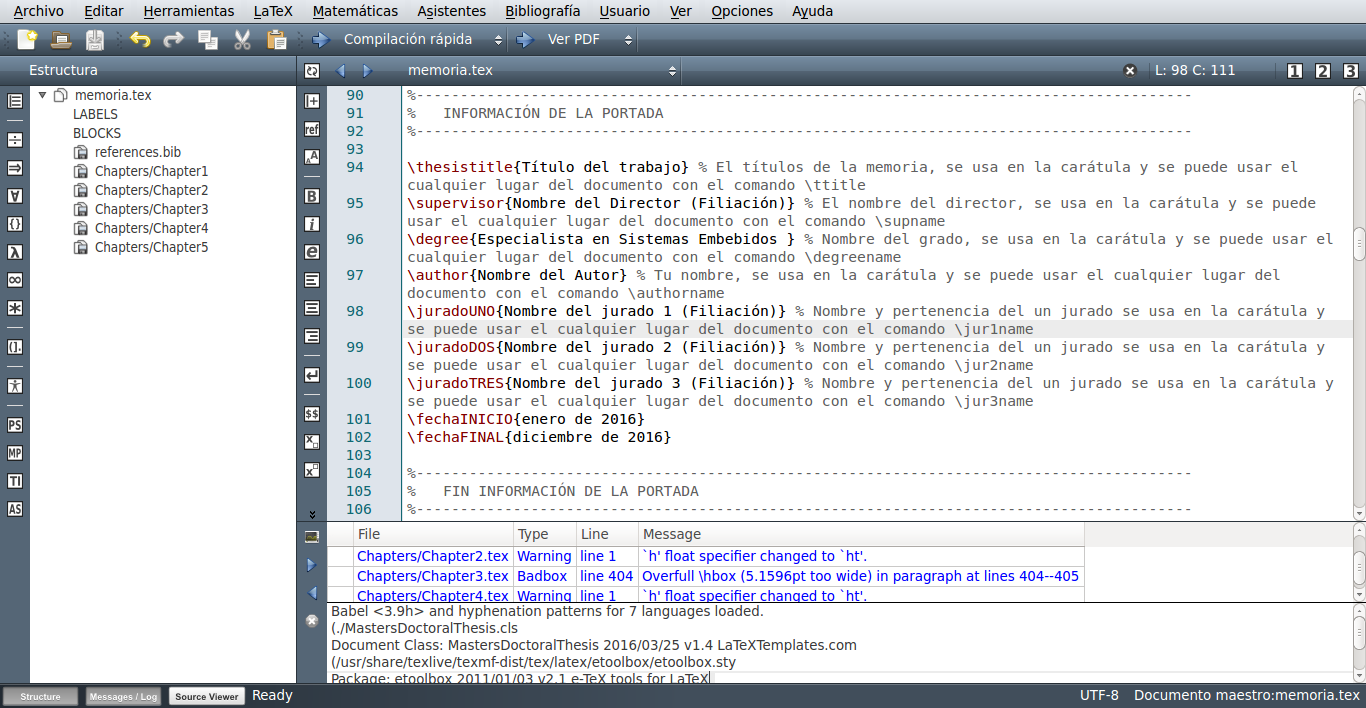
\includegraphics[width=\textwidth]{./Figures/texmaker.png}
%	\caption{Entorno de trabajo de texMaker.}
%	\label{fig:texmaker}
%\end{figure}
%
%Notar que existe una vista llamada Estructura a la izquierda de la interfaz que nos permite abrir desde dentro del programa los archivos individuales de los capítulos.  A la derecha se encuentra una vista con el archivo propiamente dicho para su edición. Hacia la parte inferior se encuentra una vista del log con información de los resultados de la compilación.  En esta última vista pueden aparecen advertencias o \textit{warning}, que normalmente pueden ser ignorados, y los errores que se indican en color rojo y deben resolverse para que se genere el PDF de salida.
%
%Recordar que el archivo que se debe compilar con PDFLaTeX es \file{memoria.tex}, si se tratara de compilar alguno de los capítulos saldría un error.  Para salvar la molestia de tener que cambiar de archivo para compilar cada vez que se realice una modificación en un capítulo, se puede definir el archivo \file{memoria.tex} como ``documento maestro'' yendo al menú opciones -> ``definir documento actual como documento maestro'', lo que permite compilar con PDFLaTeX memoria.tex directamente desde cualquier archivo que se esté modificando . Se muestra esta opción en la figura \ref{fig:docMaestro}.
%
%\begin{figure}[h]
%	\centering
%	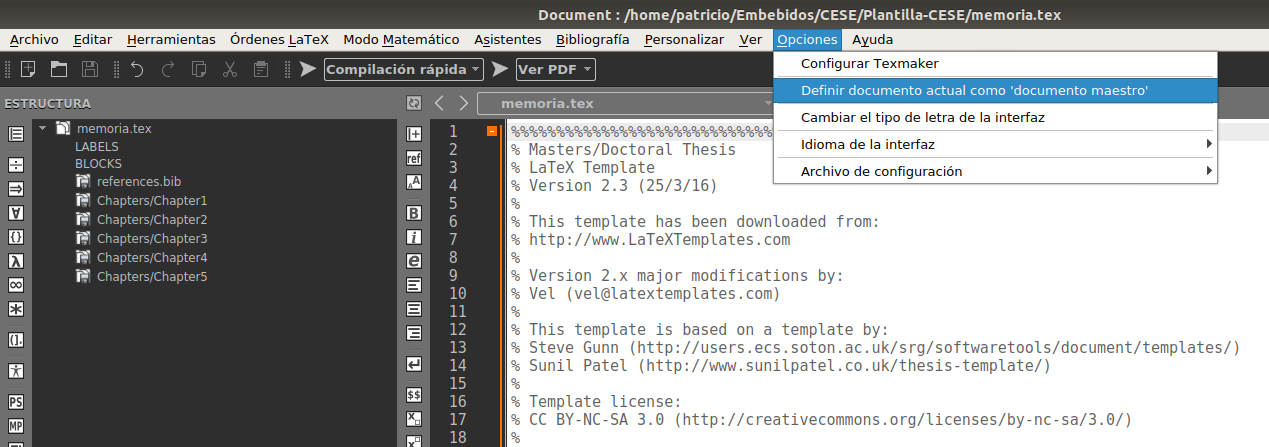
\includegraphics[width=\textwidth]{./Figures/docMaestro.png}
%	\caption{Definir memoria.tex como documento maestro.}
%	\label{fig:docMaestro}
%\end{figure}
%
%En el menú herramientas se encuentran las opciones de compilación.  Para producir un archivo PDF a partir de un archivo .tex se debe ejecutar PDFLaTeX (el shortcut es F6). Para incorporar nueva bibliografía se debe utilizar la opción BibTeX del mismo menú herramientas (el shortcut es F11).
%
%Notar que para actualizar las tablas de contenidos se debe ejecutar PDFLaTeX dos veces.  Esto se debe a que es necesario actualizar algunos archivos auxiliares antes de obtener el resultado final.  En forma similar, para actualizar las referencias se debe ejecutar primero PDFLaTeX, después BibTeX y finalmente PDFLaTeX dos veces por idénticos motivos.
%
%\section{Personalizando la plantilla, el archivo \file{memoria.tex}}
%\label{sec:FillingFile}
%
%Para personalizar la plantilla se debe incorporar la información propia en los distintos archivos \file{.tex}. 
%
%Primero abrir \file{memoria.tex} con TexMaker (o el editor de su preferencia). Se debe ubicar dentro del archivo el bloque de código titulado \emph{INFORMACIÓN DE LA PORTADA} donde se deben incorporar los primeros datos personales con los que se construirá automáticamente la portada.
%
%
%%----------------------------------------------------------------------------------------
%
%\section{El código del archivo \file{memoria.tex} explicado}
%
%El archivo \file{memoria.tex} contiene la estructura del documento y es el archivo de mayor jerarquía de la memoria.  Podría ser equiparable a la función \emph{main()} de un programa en C, o mejor dicho al archivo fuente .c donde se encuentra definida la función main().
%
%La estructura básica de cualquier documento de \LaTeX{} comienza con la definición de clase del documento, es seguida por un preámbulo donde se pueden agregar funcionalidades con el uso de \texttt{paquetes} (equiparables a bibliotecas de C), y finalmente, termina con el cuerpo del documento, donde irá el contenido de la memoria.
%
%\lstset{%
%  basicstyle=\small\ttfamily,
%  language=[LaTeX]{TeX}
%}
%
%\begin{lstlisting}
%\documentclass{article}  <- Definicion de clase
%\usepackage{listings}	 <- Preambulo
%
%\begin{document}	 <- Comienzo del contenido propio 
%	Hello world!
%\end{document}
%\end{lstlisting}
%
%
%El archivo \file{memoria.tex} se encuentra densamente comentado para explicar qué páginas, secciones y elementos de formato está creando el código \LaTeX{} en cada línea. El código está dividido en bloques con nombres en mayúsculas para que resulte evidente qué es lo que hace esa porción de código en particular. Inicialmente puede parecer que hay mucho código \LaTeX{}, pero es principalmente código para dar formato a la memoria por lo que no requiere intervención del usuario de la plantilla.  Sí se deben personalizar con su información los bloques indicados como:
%
%\begin{itemize}
%	\item Informacion de la memoria
%	\item Resumen
%	\item Agradecimientos
%	\item Dedicatoria
%\end{itemize}
%
%El índice de contenidos, las listas de figura de tablas se generan en forma automática y no requieren intervención ni edición manual por parte del usuario de la plantilla. 
%
%En la parte final del documento se encuentran los capítulos y los apéndices.  Por defecto se incluyen los 5 capítulos propuestos que se encuentran en la carpeta /Chapters. Cada capítulo se debe escribir en un archivo .tex separado y se debe poner en la carpeta \emph{Chapters} con el nombre \file{Chapter1}, \file{Chapter2}, etc\ldots El código para incluir capítulos desde archivos externos se muestra a continuación.
%
%\begin{verbatim}
%	% Chapter 1

\chapter{Introducción general} % Main chapter title

\label{Chapter1} % For referencing the chapter elsewhere, use \ref{Chapter1} 
\label{IntroGeneral}
Este capítulo introduce al lector sobre la necesidad de desarrollar un sistema que permita gestionar el recurso hídrico de manera eficiente en redes de canales. 
%----------------------------------------------------------------------------------------

% Define some commands to keep the formatting separated from the content 
\newcommand{\keyword}[1]{\textbf{#1}}
\newcommand{\tabhead}[1]{\textbf{#1}}
\newcommand{\code}[1]{\texttt{#1}}
\newcommand{\file}[1]{\texttt{\bfseries#1}}
\newcommand{\option}[1]{\texttt{\itshape#1}}
\newcommand{\grados}{$^{\circ}$}

%----------------------------------------------------------------------------------------

%\section{Introducción}

%----------------------------------------------------------------------------------------
\section{Descripción general}

La problemática del agua es central en el sostenimiento de los sistemas socioproductivos de distintas regiones de nuestro país. Las fuentes del vital recurso para la vida son escasas y en muchas circunstancias son aprovechadas de forma deficiente o bien el acceso a ellas se ve limitado por diversas causas. En este contexto, existen organismos tanto  públicos como privados que dan diagnósticos y resaltan dicha problemática de escasez, baja calidad y formas precarias de aprovechamiento de agua, muchas veces sin poder resolverla por cuestiones que tienen que ver con la disponibilidad de tecnologías apropiadas, la organización de la demanda y la gestión. 
 	 
En estas circunstancias, es posible reconocer situaciones cuando el recursos de agua es en abundancia, se puede entregar caudales mayores a los solicitados, asegurando agua a todos los usuarios, por lo que se puede identificar dos situaciones posibles, grandes pérdidas por derrames y baja eficiencia en la gestión del agua.

Actualmente son los operarios quienes recorren desde pocos hasta varios kilómetros y manualmente realizan las mediciones de los valores de parámetros necesarios con los que luego proceden a realizar el calculo correspondiente y establecer a la compuerta en una determinada posición y de esta manera fijar el caudal de agua deseado. 	 

Ante esta problemática, el propósito del presente proyecto es el diseño y construcción de un prototipo a escala de un sistema cuyo objetivo principal es suministrar una entrega eficiente de agua mediante la regulación de su caudal.

Como herramientas de trabajo, se aplicaron para la función de control, un algoritmo PID, como elemento actuador, se construyó una válvula de control servoalimentada, energizada por un motor paso a paso, y para la medición de la variable controlada, en este caso caudal, se construyó un caudalímetro por placa de aforo triangular, cuyas características dimensionales se determinaron en forma empírica.


%\subsection{Una introducción (no tan corta) a \LaTeX{}}
%
%Si sos nuevo en \LaTeX{}, hay un muy buen libro electrónico - disponible gratuitamente en Internet como un archivo PDF - llamado, \enquote{A (not so short) Introduction to \LaTeX{}}. El título del libro es generalmente acortado a simplemente \emph{lshort}. Puede descargar la versión más reciente en inglés (ya que se actualiza de vez en cuando) desde aquí:
%\url{http://www.ctan.org/tex-archive/info/lshort/english/lshort.pdf}
%
%Se puede encontrar la versión en español en la lista en esta página: \url{http://www.ctan.org/tex-archive/info/lshort/}
%
%\subsubsection{Una subsubsección}
%
%Acá tiene un ejemplo de una ``subsubsección'' que es el cuarto nivel de ordenamiento del texto, después de capítulo, sección y subsección.  Como se puede ver, las subsubsecciones no van numeradas en el cuerpo del documento ni en el índice.  El formato está definido por la plantilla y no debe ser modificado.
%
%\subsection{Guía matemática rápida para \LaTeX{}}
%
%Si estás escribiendo un documento con mucho contenido matemático, entonces es posible que desees leer el documento de la AMS (American Mathematical Society) llamado, \enquote{A Short Math Guide for \LaTeX{}}. Se puede encontrar en línea en el siguiente link: \url{http://www.ams.org/tex/amslatex.html} en la sección \enquote{Additional Documentation} hacia la parte inferior de la página.

%
%----------------------------------------------------------------------------------------

\section{Motivación}

La gestión de canales y redes de distribución de agua en la mayoría de las regiones del país se basa en operaciones de control manual en la que los operarios supervisan el estado de cada elemento y actúan en función de protocolos establecidos.
		
Hoy por hoy, estos procedimientos presentan una capacidad de reacción lenta ante la demanda variable de cada uno de los usuarios de agua,  ya que los operarios, en ocasiones deben recorrer varios kilómetros por lo que esto, representa un costo sumamente elevado mantener este servicio.

Este proyecto, además de regular el caudal de agua en canal abierto podrá resolver los problemas referentes a la disponibilidad de agua en regiones que presentan escasez por diferentes factores, no solo por sequías. Asimismo, no sólo busca maximizar la eficiencia en el abastecimiento de agua a cada uno de los usuarios en tiempo y forma, sino también minimizar la pérdida de la misma en la red de canales, y así, de esta manera, poder brindar mayor seguridad en el suministro de agua para el riego a cada productor en sus predios.

De este modo, se podrá obtener mejoras en la calidad de sus productos y por sobre todo, mayores rendimientos en su producción. El riego es la labor cultural que mayor impacto tiene sobre el rendimiento y la calidad en los productos. 

A fin de minimizar errores que introduce al trabajar con un prototipo formado por una compuerta esta fue reemplazada por una válvula, ya que de esta forma permite trabajar sin filtraciones de agua y mayor precisión en la medición.   	  
Es importante aclarar que una red o las redes de canales se encuentran separadas por compuertas. En el prototipo la válvula simula ser una compuerta.

Uno de los objetivos planteados para una segunda fase de desarrollo es instanciar, este sistema desarrollado en el presente informe, en varias compuertas que constituye una red de canal de modo tal, que las mismas se comuniquen entre sí utilizando tecnología LoraWan y lograr como sistema general se ejecute de forma autónoma.  

Con el presente sistema de control también se busca promover la recuperación del potencial productivo de los suelos agropecuarios  que se han degradado por diferentes factores, entre ellos la escasez de agua. 

Es de destacar que no existen soluciones nacionales, por lo tanto,  el desafío es lograr ser competitivo en precio y prestaciones con productos importados que se encuentran en el mercado. Esto trae aparejado, desde el punto vista del cliente el beneficio de contar con soporte local y la posibilidad de modificar algo del sistema según las necesidades del cliente.

%----------------------------------------------------------------------------------------

\section{Objetivos y alcances}

%\subsection{Objetivos}

El objetivo general de este trabajo es aportar el diseño y elaboración de un sistema que mediante el empleo de un algoritmo de control PID permite regular el caudal de agua en canal abierto y con el uso de las tecnologías más actuales pueda ser empleado tanto en red de canales complejos hasta las redes más simples. A continuación se detallan los subobjetivos específicos que se tuvieron en cuenta :  
\begin{itemize}
\item Diseño y construcción de  un sistema de control que permita al usuario establecer un caudal de agua determinado de forma remota.

\item Diseño y fabricación de un circuito de control de señales cuya finalidad del mismo es cumplir la función de interfaz entre la etapa de control y la de potencia correspondiente al driver del motor paso a paso. 
\item El firmware incluye un sistema de tiempo real.  
\item Para regular el caudal de agua, aplicar un algoritmo de control PID.
\item Empleo de un sensor de presión que posea una precisión de 1 mm para detectar el nivel de la superficie del agua.
\item Utilización de un potenciómetro de manera tal que conjuntamente a un motor paso a paso conformen un servo motor y posicionar a la válvula en un determinado ángulo.  
\item Proporcionar una gestión de agua de riego de forma eficiente.
\item Desarrollar un firmware escalable de tal modo que permita la comunicación con otros firmware's instanciados en otras compuerta. 
\end{itemize}

 
%Esta plantilla se distribuye como una único archivo .zip que se puede descomprimir en varios archivos y carpetas. Asimismo, se puede consultar el repositorio git para obtener la última versión de los archivos, \url{https://github.com/patriciobos/Plantilla-CESE.git}. Los nombres de las carpetas son, o pretender ser, auto-explicativos.
%
%\keyword{Appendices} -- Esta es la carpeta donde se deben poner los apéndices. Cada apéndice debe ir en su propio archivo \file{.tex}. Se incluye un ejemplo y una plantilla en la carpeta.
%
%\keyword{Chapters} -- Esta es la carpeta donde se deben poner los capítulos de la memoria. Cada capítulo debe ir un su propio archivo \file{.tex} por separado.  Se ofrece por defecto, la siguiente estructura de capítulos y se recomienda su utilización dentro de lo posible:
%
%\begin{itemize}
%\item Capítulo 1: Introducción general	
%\item Capítulo 2: Introducción específica
%\item Capítulo 3: Diseño e implementación
%\item Capítulo 4: Ensayos y resultados
%\item Capítulo 5: Conclusiones
%
%\end{itemize}
%
%Esta estructura de capítulos es la que se recomienda para las memorias de la especialización.
%
%\keyword{Figures} -- Esta carpeta contiene todas las figuras de la memoria.  Estas son las versiones finales de las imágenes que van a ser incluidas en la memoria.  Pueden ser imágenes en formato \textit{raster}\footnote{\url{https://en.wikipedia.org/wiki/Raster_graphics}} como \file{.png}, \file{.jpg} o en formato vectoriales\footnote{\url{https://en.wikipedia.org/wiki/Vector_graphics}} como \file{.pdf}, \file{.ps}.  Se debe notar que utilizar imágenes vectoriales disminuye notablemente el peso del documento final y acelera el tiempo de compilación por lo que es recomendable su utilización siempre que sea posible.
%
%\subsection{Archivos}
%
%También están incluidos varios archivos, la mayoría de ellos son de texto plano y se puede ver su contenido en un editor de texto. Después de la compilación inicial, se verá que más archivos auxiliares son creados por \ LaTeX{} o BibTeX, pero son de uso interno y no es necesario hacer nada en particular con ellos.  Toda la información necesaria para compilar el documento se encuentra en los archivos \file{.tex}, \file{.bib}, \file{.cls} y en las imágenes de la carpeta Figures.
%
%\keyword{referencias.bib} - este es un archivo importante que contiene toda la información de referencias bibliográficas que se utilizarán para las citas en la memoria en conjunto con BibTeX. Usted puede escribir las entradas bibliográficas en forma manual, aunque existen también programas de gestión de referencias que facilitan la creación y gestión de las referencias y permiten exportarlas en formato BibTeX.  También hay disponibles sitios web como \url{books.google.com} que permiten obtener toda la información necesaria para una cita en formato BibTeX. Ver sección \ref{sec:biblio}
%
%\keyword{MastersDoctoralThesis.cls} -- este es un archivo importante. Es el archivos con la clase que le informa a \LaTeX{} cómo debe dar formato a la memoria. El usuario de la plantilla no debería necesitar modificar nada de este archivo.
%
%\keyword{memoria.pdf} -- esta es su memoria con una tipografía bellamente compuesta (en formato de archivo PDF) creado por \LaTeX{}. Se distribuye con la plantilla y después de compilar por primera vez sin hacer ningún cambio se debería obtener una versión idéntica a este documento.
%
%\keyword{memoria.tex} -- este es un archivo importante. Este es el archivo que tiene que compilar \LaTeX{} para producir la memoria como un archivo PDF. Contiene un marco de trabajo y estructuras que le indican a \LaTeX{} cómo diagramar la memoria.  Está altamente comentado para que se pueda entender qué es lo que realiza cada línea de código y por qué está incluida en ese lugar.  En este archivo se debe completar la información personalizada de las primeras sección según se indica en la sección \ref{sec:FillingFile}.
%
%Archivos que \emph{no} forman parte de la distribución de la plantilla pero que son generados por \LaTeX{} como archivos auxiliares necesarios para la producción de la memoria.pdf son:
%
%\keyword{memoria.aux} -- este es un archivo auxiliar generado por \LaTeX{}, si se borra \LaTeX{} simplemente lo regenera cuando se compila el archivo principal \file{memoria.tex}.
%
%\keyword{memoria.bbl} -- este es un archivo auxiliar generado por BibTeX, si se borra BibTeX simplemente lo regenera cuando se compila el archivo principal \file{memoria.tex}. Mientras que el archivo \file{.bib} contiene todas las referencias que hay, este archivo \file{.bbl} contine sólo las referencias que han sido citadas y se utiliza para la construcción de la bibiografía.
%
%\keyword{memoria.blg} -- este es un archivo auxiliar generado por BibTeX, si se borra BibTeX simplemente lo regenera cuando se compila el archivo principal \file{memoria.tex}.
%
%\keyword{memoria.lof} -- este es un archivo auxiliar generado por \LaTeX{}, si se borra \LaTeX{} simplemente lo regenera cuando se compila el archivo principal \file{memoria.tex}.  Le indica a \LaTeX{} cómo construir la sección \emph{Lista de Figuras}.
% 
%\keyword{memoria.log} --  este es un archivo auxiliar generado por \LaTeX{}, si se borra \LaTeX{} simplemente lo regenera cuando se compila el archivo principal \file{memoria.tex}. Contiene mensajes de \LaTeX{}. Si se reciben errores o advertencias durante la compilación, se guardan en este archivo \file{.log}.
%
%\keyword{memoria.lot} -- este es un archivo auxiliar generado por \LaTeX{}, si se borra \LaTeX{} simplemente lo regenera cuando se compila el archivo principal \file{memoria.tex}.  Le indica a \LaTeX{} cómo construir la sección \emph{Lista de Tablas}.
%
%\keyword{memoria.out} -- este es un archivo auxiliar generado por \LaTeX{}, si se borra \LaTeX{} simplemente lo regenera cuando se compila el archivo principal \file{memoria.tex}.
%
%De esta larga lista de archivos, sólo aquellos con la extensión \file{.bib}, \file{.cls} y \file{.tex} son importantes.  Los otros archivos auxiliares pueden ser ignorados o borrados ya que \LaTeX{} y BibTeX los regenerarán durante la compilación.
%
%%----------------------------------------------------------------------------------------
%
%\section{Entorno de trabajo}
%
%Ante de comenzar a editar la plantilla debemos tener un editor \LaTeX{} instalado en nuestra computadora.  En forma análoga a lo que sucede en lenguaje C, que se puede crear y editar código con casi cualquier editor, existen ciertos entornos de trabajo que nos pueden simplificar mucho la tarea.  En este sentido, se recomienda, sobre todo para los principiantes en \LaTeX{} la utilización de TexMaker, un programa gratuito y multi-plantaforma que está disponible tanto para windows como para sistemas GNU/linux.
%
%La versión más reciente de TexMaker es la 4.5 y se puede descargar del siguiente link: \url{http://www.xm1math.net/texmaker/download.html}. Se puede consultar el manual de usuario en el siguiente link: \url{http://www.xm1math.net/texmaker/doc.html}.
% 
%
%\subsection{Paquetes adicionales}
%
%Si bien durante el proceso de instalación de TexMaker, o cualquier otro editor que se haya elegido, se instalarán en el sistema los paquetes básicos necesarios para trabajar con \LaTeX{}, la plantilla de los trabajos de Especialización y Maestría requieren de paquete adicionales.
%
%Se indican a continuación los comandos que se deben introducir en la consola de Ubuntu (ctrl + alt + t) para instalarlos:
%
%\begin{lstlisting}[language=bash]
%  $ sudo apt install texlive-lang-spanish texlive-science 
%  $ sudo apt install texlive-bibtex-extra biber
%  $ sudo apt install texlive texlive-fonts-recommended
%  $ sudo apt install texlive-latex-extra
%\end{lstlisting}
%
%
%\subsection{Configurando TexMaker}
%
%
%Una vez instalado el programa y los paquetes adicionales se debe abrir el archivo memoria.tex con el editor para ver una pantalla similar a la que se puede apreciar en la figura \ref{fig:texmaker}. 
%
%\begin{figure}[h]
%	\centering
%	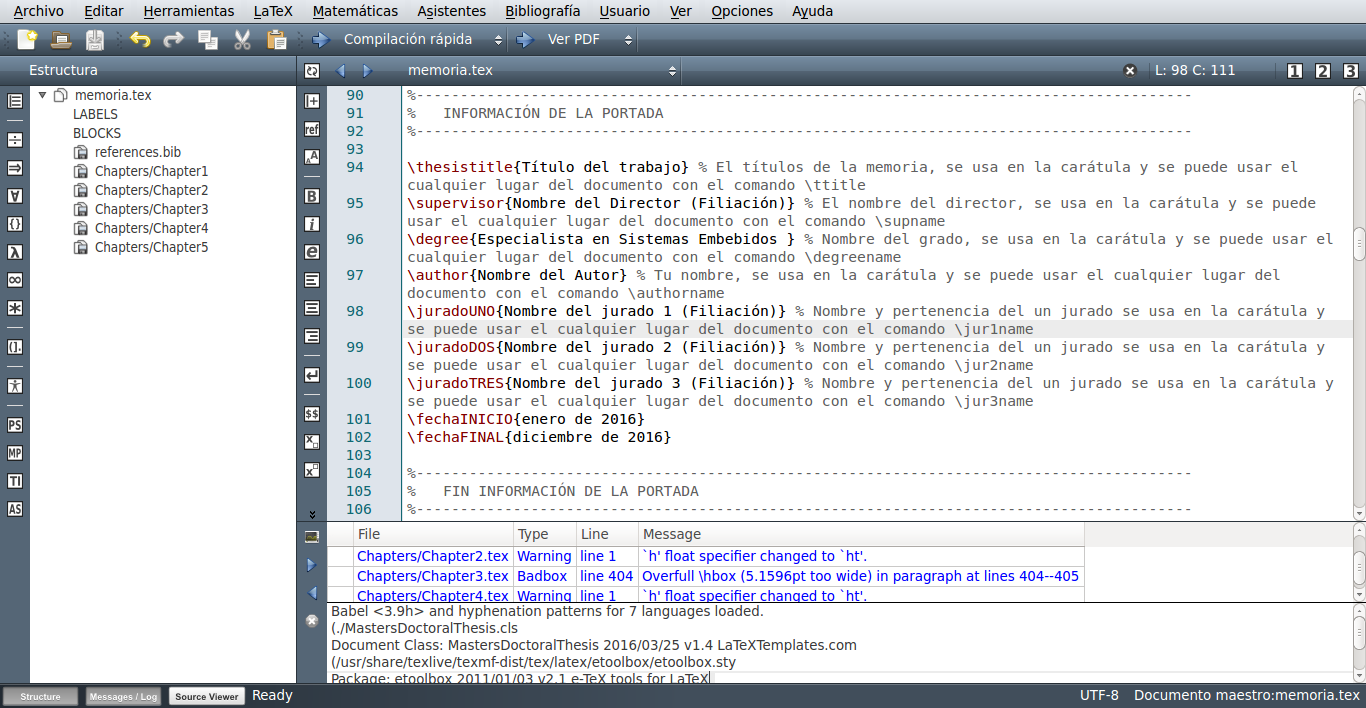
\includegraphics[width=\textwidth]{./Figures/texmaker.png}
%	\caption{Entorno de trabajo de texMaker.}
%	\label{fig:texmaker}
%\end{figure}
%
%Notar que existe una vista llamada Estructura a la izquierda de la interfaz que nos permite abrir desde dentro del programa los archivos individuales de los capítulos.  A la derecha se encuentra una vista con el archivo propiamente dicho para su edición. Hacia la parte inferior se encuentra una vista del log con información de los resultados de la compilación.  En esta última vista pueden aparecen advertencias o \textit{warning}, que normalmente pueden ser ignorados, y los errores que se indican en color rojo y deben resolverse para que se genere el PDF de salida.
%
%Recordar que el archivo que se debe compilar con PDFLaTeX es \file{memoria.tex}, si se tratara de compilar alguno de los capítulos saldría un error.  Para salvar la molestia de tener que cambiar de archivo para compilar cada vez que se realice una modificación en un capítulo, se puede definir el archivo \file{memoria.tex} como ``documento maestro'' yendo al menú opciones -> ``definir documento actual como documento maestro'', lo que permite compilar con PDFLaTeX memoria.tex directamente desde cualquier archivo que se esté modificando . Se muestra esta opción en la figura \ref{fig:docMaestro}.
%
%\begin{figure}[h]
%	\centering
%	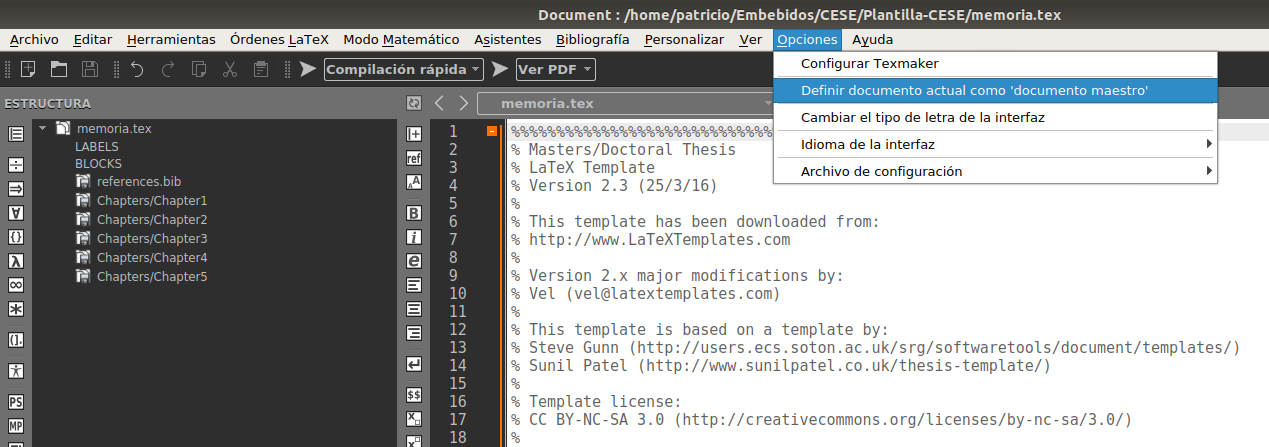
\includegraphics[width=\textwidth]{./Figures/docMaestro.png}
%	\caption{Definir memoria.tex como documento maestro.}
%	\label{fig:docMaestro}
%\end{figure}
%
%En el menú herramientas se encuentran las opciones de compilación.  Para producir un archivo PDF a partir de un archivo .tex se debe ejecutar PDFLaTeX (el shortcut es F6). Para incorporar nueva bibliografía se debe utilizar la opción BibTeX del mismo menú herramientas (el shortcut es F11).
%
%Notar que para actualizar las tablas de contenidos se debe ejecutar PDFLaTeX dos veces.  Esto se debe a que es necesario actualizar algunos archivos auxiliares antes de obtener el resultado final.  En forma similar, para actualizar las referencias se debe ejecutar primero PDFLaTeX, después BibTeX y finalmente PDFLaTeX dos veces por idénticos motivos.
%
%\section{Personalizando la plantilla, el archivo \file{memoria.tex}}
%\label{sec:FillingFile}
%
%Para personalizar la plantilla se debe incorporar la información propia en los distintos archivos \file{.tex}. 
%
%Primero abrir \file{memoria.tex} con TexMaker (o el editor de su preferencia). Se debe ubicar dentro del archivo el bloque de código titulado \emph{INFORMACIÓN DE LA PORTADA} donde se deben incorporar los primeros datos personales con los que se construirá automáticamente la portada.
%
%
%%----------------------------------------------------------------------------------------
%
%\section{El código del archivo \file{memoria.tex} explicado}
%
%El archivo \file{memoria.tex} contiene la estructura del documento y es el archivo de mayor jerarquía de la memoria.  Podría ser equiparable a la función \emph{main()} de un programa en C, o mejor dicho al archivo fuente .c donde se encuentra definida la función main().
%
%La estructura básica de cualquier documento de \LaTeX{} comienza con la definición de clase del documento, es seguida por un preámbulo donde se pueden agregar funcionalidades con el uso de \texttt{paquetes} (equiparables a bibliotecas de C), y finalmente, termina con el cuerpo del documento, donde irá el contenido de la memoria.
%
%\lstset{%
%  basicstyle=\small\ttfamily,
%  language=[LaTeX]{TeX}
%}
%
%\begin{lstlisting}
%\documentclass{article}  <- Definicion de clase
%\usepackage{listings}	 <- Preambulo
%
%\begin{document}	 <- Comienzo del contenido propio 
%	Hello world!
%\end{document}
%\end{lstlisting}
%
%
%El archivo \file{memoria.tex} se encuentra densamente comentado para explicar qué páginas, secciones y elementos de formato está creando el código \LaTeX{} en cada línea. El código está dividido en bloques con nombres en mayúsculas para que resulte evidente qué es lo que hace esa porción de código en particular. Inicialmente puede parecer que hay mucho código \LaTeX{}, pero es principalmente código para dar formato a la memoria por lo que no requiere intervención del usuario de la plantilla.  Sí se deben personalizar con su información los bloques indicados como:
%
%\begin{itemize}
%	\item Informacion de la memoria
%	\item Resumen
%	\item Agradecimientos
%	\item Dedicatoria
%\end{itemize}
%
%El índice de contenidos, las listas de figura de tablas se generan en forma automática y no requieren intervención ni edición manual por parte del usuario de la plantilla. 
%
%En la parte final del documento se encuentran los capítulos y los apéndices.  Por defecto se incluyen los 5 capítulos propuestos que se encuentran en la carpeta /Chapters. Cada capítulo se debe escribir en un archivo .tex separado y se debe poner en la carpeta \emph{Chapters} con el nombre \file{Chapter1}, \file{Chapter2}, etc\ldots El código para incluir capítulos desde archivos externos se muestra a continuación.
%
%\begin{verbatim}
%	% Chapter 1

\chapter{Introducción general} % Main chapter title

\label{Chapter1} % For referencing the chapter elsewhere, use \ref{Chapter1} 
\label{IntroGeneral}
Este capítulo introduce al lector sobre la necesidad de desarrollar un sistema que permita gestionar el recurso hídrico de manera eficiente en redes de canales. 
%----------------------------------------------------------------------------------------

% Define some commands to keep the formatting separated from the content 
\newcommand{\keyword}[1]{\textbf{#1}}
\newcommand{\tabhead}[1]{\textbf{#1}}
\newcommand{\code}[1]{\texttt{#1}}
\newcommand{\file}[1]{\texttt{\bfseries#1}}
\newcommand{\option}[1]{\texttt{\itshape#1}}
\newcommand{\grados}{$^{\circ}$}

%----------------------------------------------------------------------------------------

%\section{Introducción}

%----------------------------------------------------------------------------------------
\section{Descripción general}

La problemática del agua es central en el sostenimiento de los sistemas socioproductivos de distintas regiones de nuestro país. Las fuentes del vital recurso para la vida son escasas y en muchas circunstancias son aprovechadas de forma deficiente o bien el acceso a ellas se ve limitado por diversas causas. En este contexto, existen organismos tanto  públicos como privados que dan diagnósticos y resaltan dicha problemática de escasez, baja calidad y formas precarias de aprovechamiento de agua, muchas veces sin poder resolverla por cuestiones que tienen que ver con la disponibilidad de tecnologías apropiadas, la organización de la demanda y la gestión. 
 	 
En estas circunstancias, es posible reconocer situaciones cuando el recursos de agua es en abundancia, se puede entregar caudales mayores a los solicitados, asegurando agua a todos los usuarios, por lo que se puede identificar dos situaciones posibles, grandes pérdidas por derrames y baja eficiencia en la gestión del agua.

Actualmente son los operarios quienes recorren desde pocos hasta varios kilómetros y manualmente realizan las mediciones de los valores de parámetros necesarios con los que luego proceden a realizar el calculo correspondiente y establecer a la compuerta en una determinada posición y de esta manera fijar el caudal de agua deseado. 	 

Ante esta problemática, el propósito del presente proyecto es el diseño y construcción de un prototipo a escala de un sistema cuyo objetivo principal es suministrar una entrega eficiente de agua mediante la regulación de su caudal.

Como herramientas de trabajo, se aplicaron para la función de control, un algoritmo PID, como elemento actuador, se construyó una válvula de control servoalimentada, energizada por un motor paso a paso, y para la medición de la variable controlada, en este caso caudal, se construyó un caudalímetro por placa de aforo triangular, cuyas características dimensionales se determinaron en forma empírica.


%\subsection{Una introducción (no tan corta) a \LaTeX{}}
%
%Si sos nuevo en \LaTeX{}, hay un muy buen libro electrónico - disponible gratuitamente en Internet como un archivo PDF - llamado, \enquote{A (not so short) Introduction to \LaTeX{}}. El título del libro es generalmente acortado a simplemente \emph{lshort}. Puede descargar la versión más reciente en inglés (ya que se actualiza de vez en cuando) desde aquí:
%\url{http://www.ctan.org/tex-archive/info/lshort/english/lshort.pdf}
%
%Se puede encontrar la versión en español en la lista en esta página: \url{http://www.ctan.org/tex-archive/info/lshort/}
%
%\subsubsection{Una subsubsección}
%
%Acá tiene un ejemplo de una ``subsubsección'' que es el cuarto nivel de ordenamiento del texto, después de capítulo, sección y subsección.  Como se puede ver, las subsubsecciones no van numeradas en el cuerpo del documento ni en el índice.  El formato está definido por la plantilla y no debe ser modificado.
%
%\subsection{Guía matemática rápida para \LaTeX{}}
%
%Si estás escribiendo un documento con mucho contenido matemático, entonces es posible que desees leer el documento de la AMS (American Mathematical Society) llamado, \enquote{A Short Math Guide for \LaTeX{}}. Se puede encontrar en línea en el siguiente link: \url{http://www.ams.org/tex/amslatex.html} en la sección \enquote{Additional Documentation} hacia la parte inferior de la página.

%
%----------------------------------------------------------------------------------------

\section{Motivación}

La gestión de canales y redes de distribución de agua en la mayoría de las regiones del país se basa en operaciones de control manual en la que los operarios supervisan el estado de cada elemento y actúan en función de protocolos establecidos.
		
Hoy por hoy, estos procedimientos presentan una capacidad de reacción lenta ante la demanda variable de cada uno de los usuarios de agua,  ya que los operarios, en ocasiones deben recorrer varios kilómetros por lo que esto, representa un costo sumamente elevado mantener este servicio.

Este proyecto, además de regular el caudal de agua en canal abierto podrá resolver los problemas referentes a la disponibilidad de agua en regiones que presentan escasez por diferentes factores, no solo por sequías. Asimismo, no sólo busca maximizar la eficiencia en el abastecimiento de agua a cada uno de los usuarios en tiempo y forma, sino también minimizar la pérdida de la misma en la red de canales, y así, de esta manera, poder brindar mayor seguridad en el suministro de agua para el riego a cada productor en sus predios.

De este modo, se podrá obtener mejoras en la calidad de sus productos y por sobre todo, mayores rendimientos en su producción. El riego es la labor cultural que mayor impacto tiene sobre el rendimiento y la calidad en los productos. 

A fin de minimizar errores que introduce al trabajar con un prototipo formado por una compuerta esta fue reemplazada por una válvula, ya que de esta forma permite trabajar sin filtraciones de agua y mayor precisión en la medición.   	  
Es importante aclarar que una red o las redes de canales se encuentran separadas por compuertas. En el prototipo la válvula simula ser una compuerta.

Uno de los objetivos planteados para una segunda fase de desarrollo es instanciar, este sistema desarrollado en el presente informe, en varias compuertas que constituye una red de canal de modo tal, que las mismas se comuniquen entre sí utilizando tecnología LoraWan y lograr como sistema general se ejecute de forma autónoma.  

Con el presente sistema de control también se busca promover la recuperación del potencial productivo de los suelos agropecuarios  que se han degradado por diferentes factores, entre ellos la escasez de agua. 

Es de destacar que no existen soluciones nacionales, por lo tanto,  el desafío es lograr ser competitivo en precio y prestaciones con productos importados que se encuentran en el mercado. Esto trae aparejado, desde el punto vista del cliente el beneficio de contar con soporte local y la posibilidad de modificar algo del sistema según las necesidades del cliente.

%----------------------------------------------------------------------------------------

\section{Objetivos y alcances}

%\subsection{Objetivos}

El objetivo general de este trabajo es aportar el diseño y elaboración de un sistema que mediante el empleo de un algoritmo de control PID permite regular el caudal de agua en canal abierto y con el uso de las tecnologías más actuales pueda ser empleado tanto en red de canales complejos hasta las redes más simples. A continuación se detallan los subobjetivos específicos que se tuvieron en cuenta :  
\begin{itemize}
\item Diseño y construcción de  un sistema de control que permita al usuario establecer un caudal de agua determinado de forma remota.

\item Diseño y fabricación de un circuito de control de señales cuya finalidad del mismo es cumplir la función de interfaz entre la etapa de control y la de potencia correspondiente al driver del motor paso a paso. 
\item El firmware incluye un sistema de tiempo real.  
\item Para regular el caudal de agua, aplicar un algoritmo de control PID.
\item Empleo de un sensor de presión que posea una precisión de 1 mm para detectar el nivel de la superficie del agua.
\item Utilización de un potenciómetro de manera tal que conjuntamente a un motor paso a paso conformen un servo motor y posicionar a la válvula en un determinado ángulo.  
\item Proporcionar una gestión de agua de riego de forma eficiente.
\item Desarrollar un firmware escalable de tal modo que permita la comunicación con otros firmware's instanciados en otras compuerta. 
\end{itemize}

 
%Esta plantilla se distribuye como una único archivo .zip que se puede descomprimir en varios archivos y carpetas. Asimismo, se puede consultar el repositorio git para obtener la última versión de los archivos, \url{https://github.com/patriciobos/Plantilla-CESE.git}. Los nombres de las carpetas son, o pretender ser, auto-explicativos.
%
%\keyword{Appendices} -- Esta es la carpeta donde se deben poner los apéndices. Cada apéndice debe ir en su propio archivo \file{.tex}. Se incluye un ejemplo y una plantilla en la carpeta.
%
%\keyword{Chapters} -- Esta es la carpeta donde se deben poner los capítulos de la memoria. Cada capítulo debe ir un su propio archivo \file{.tex} por separado.  Se ofrece por defecto, la siguiente estructura de capítulos y se recomienda su utilización dentro de lo posible:
%
%\begin{itemize}
%\item Capítulo 1: Introducción general	
%\item Capítulo 2: Introducción específica
%\item Capítulo 3: Diseño e implementación
%\item Capítulo 4: Ensayos y resultados
%\item Capítulo 5: Conclusiones
%
%\end{itemize}
%
%Esta estructura de capítulos es la que se recomienda para las memorias de la especialización.
%
%\keyword{Figures} -- Esta carpeta contiene todas las figuras de la memoria.  Estas son las versiones finales de las imágenes que van a ser incluidas en la memoria.  Pueden ser imágenes en formato \textit{raster}\footnote{\url{https://en.wikipedia.org/wiki/Raster_graphics}} como \file{.png}, \file{.jpg} o en formato vectoriales\footnote{\url{https://en.wikipedia.org/wiki/Vector_graphics}} como \file{.pdf}, \file{.ps}.  Se debe notar que utilizar imágenes vectoriales disminuye notablemente el peso del documento final y acelera el tiempo de compilación por lo que es recomendable su utilización siempre que sea posible.
%
%\subsection{Archivos}
%
%También están incluidos varios archivos, la mayoría de ellos son de texto plano y se puede ver su contenido en un editor de texto. Después de la compilación inicial, se verá que más archivos auxiliares son creados por \ LaTeX{} o BibTeX, pero son de uso interno y no es necesario hacer nada en particular con ellos.  Toda la información necesaria para compilar el documento se encuentra en los archivos \file{.tex}, \file{.bib}, \file{.cls} y en las imágenes de la carpeta Figures.
%
%\keyword{referencias.bib} - este es un archivo importante que contiene toda la información de referencias bibliográficas que se utilizarán para las citas en la memoria en conjunto con BibTeX. Usted puede escribir las entradas bibliográficas en forma manual, aunque existen también programas de gestión de referencias que facilitan la creación y gestión de las referencias y permiten exportarlas en formato BibTeX.  También hay disponibles sitios web como \url{books.google.com} que permiten obtener toda la información necesaria para una cita en formato BibTeX. Ver sección \ref{sec:biblio}
%
%\keyword{MastersDoctoralThesis.cls} -- este es un archivo importante. Es el archivos con la clase que le informa a \LaTeX{} cómo debe dar formato a la memoria. El usuario de la plantilla no debería necesitar modificar nada de este archivo.
%
%\keyword{memoria.pdf} -- esta es su memoria con una tipografía bellamente compuesta (en formato de archivo PDF) creado por \LaTeX{}. Se distribuye con la plantilla y después de compilar por primera vez sin hacer ningún cambio se debería obtener una versión idéntica a este documento.
%
%\keyword{memoria.tex} -- este es un archivo importante. Este es el archivo que tiene que compilar \LaTeX{} para producir la memoria como un archivo PDF. Contiene un marco de trabajo y estructuras que le indican a \LaTeX{} cómo diagramar la memoria.  Está altamente comentado para que se pueda entender qué es lo que realiza cada línea de código y por qué está incluida en ese lugar.  En este archivo se debe completar la información personalizada de las primeras sección según se indica en la sección \ref{sec:FillingFile}.
%
%Archivos que \emph{no} forman parte de la distribución de la plantilla pero que son generados por \LaTeX{} como archivos auxiliares necesarios para la producción de la memoria.pdf son:
%
%\keyword{memoria.aux} -- este es un archivo auxiliar generado por \LaTeX{}, si se borra \LaTeX{} simplemente lo regenera cuando se compila el archivo principal \file{memoria.tex}.
%
%\keyword{memoria.bbl} -- este es un archivo auxiliar generado por BibTeX, si se borra BibTeX simplemente lo regenera cuando se compila el archivo principal \file{memoria.tex}. Mientras que el archivo \file{.bib} contiene todas las referencias que hay, este archivo \file{.bbl} contine sólo las referencias que han sido citadas y se utiliza para la construcción de la bibiografía.
%
%\keyword{memoria.blg} -- este es un archivo auxiliar generado por BibTeX, si se borra BibTeX simplemente lo regenera cuando se compila el archivo principal \file{memoria.tex}.
%
%\keyword{memoria.lof} -- este es un archivo auxiliar generado por \LaTeX{}, si se borra \LaTeX{} simplemente lo regenera cuando se compila el archivo principal \file{memoria.tex}.  Le indica a \LaTeX{} cómo construir la sección \emph{Lista de Figuras}.
% 
%\keyword{memoria.log} --  este es un archivo auxiliar generado por \LaTeX{}, si se borra \LaTeX{} simplemente lo regenera cuando se compila el archivo principal \file{memoria.tex}. Contiene mensajes de \LaTeX{}. Si se reciben errores o advertencias durante la compilación, se guardan en este archivo \file{.log}.
%
%\keyword{memoria.lot} -- este es un archivo auxiliar generado por \LaTeX{}, si se borra \LaTeX{} simplemente lo regenera cuando se compila el archivo principal \file{memoria.tex}.  Le indica a \LaTeX{} cómo construir la sección \emph{Lista de Tablas}.
%
%\keyword{memoria.out} -- este es un archivo auxiliar generado por \LaTeX{}, si se borra \LaTeX{} simplemente lo regenera cuando se compila el archivo principal \file{memoria.tex}.
%
%De esta larga lista de archivos, sólo aquellos con la extensión \file{.bib}, \file{.cls} y \file{.tex} son importantes.  Los otros archivos auxiliares pueden ser ignorados o borrados ya que \LaTeX{} y BibTeX los regenerarán durante la compilación.
%
%%----------------------------------------------------------------------------------------
%
%\section{Entorno de trabajo}
%
%Ante de comenzar a editar la plantilla debemos tener un editor \LaTeX{} instalado en nuestra computadora.  En forma análoga a lo que sucede en lenguaje C, que se puede crear y editar código con casi cualquier editor, existen ciertos entornos de trabajo que nos pueden simplificar mucho la tarea.  En este sentido, se recomienda, sobre todo para los principiantes en \LaTeX{} la utilización de TexMaker, un programa gratuito y multi-plantaforma que está disponible tanto para windows como para sistemas GNU/linux.
%
%La versión más reciente de TexMaker es la 4.5 y se puede descargar del siguiente link: \url{http://www.xm1math.net/texmaker/download.html}. Se puede consultar el manual de usuario en el siguiente link: \url{http://www.xm1math.net/texmaker/doc.html}.
% 
%
%\subsection{Paquetes adicionales}
%
%Si bien durante el proceso de instalación de TexMaker, o cualquier otro editor que se haya elegido, se instalarán en el sistema los paquetes básicos necesarios para trabajar con \LaTeX{}, la plantilla de los trabajos de Especialización y Maestría requieren de paquete adicionales.
%
%Se indican a continuación los comandos que se deben introducir en la consola de Ubuntu (ctrl + alt + t) para instalarlos:
%
%\begin{lstlisting}[language=bash]
%  $ sudo apt install texlive-lang-spanish texlive-science 
%  $ sudo apt install texlive-bibtex-extra biber
%  $ sudo apt install texlive texlive-fonts-recommended
%  $ sudo apt install texlive-latex-extra
%\end{lstlisting}
%
%
%\subsection{Configurando TexMaker}
%
%
%Una vez instalado el programa y los paquetes adicionales se debe abrir el archivo memoria.tex con el editor para ver una pantalla similar a la que se puede apreciar en la figura \ref{fig:texmaker}. 
%
%\begin{figure}[h]
%	\centering
%	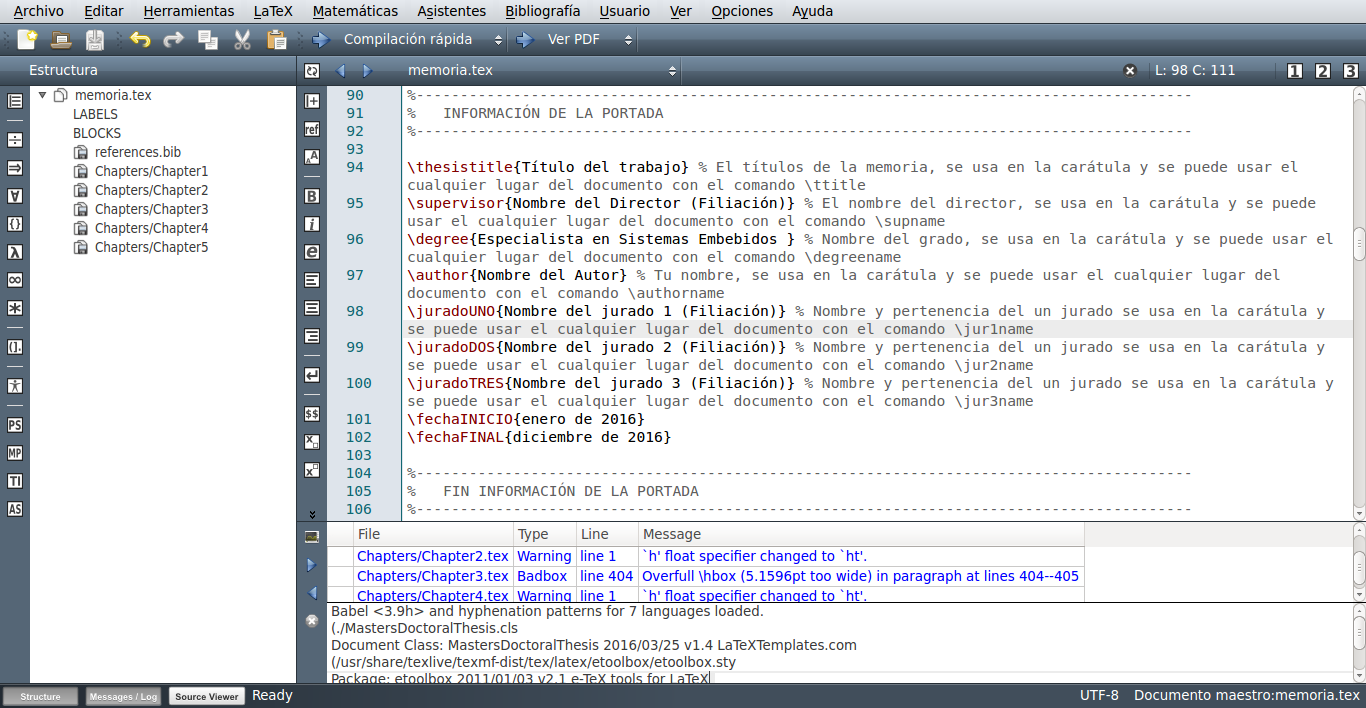
\includegraphics[width=\textwidth]{./Figures/texmaker.png}
%	\caption{Entorno de trabajo de texMaker.}
%	\label{fig:texmaker}
%\end{figure}
%
%Notar que existe una vista llamada Estructura a la izquierda de la interfaz que nos permite abrir desde dentro del programa los archivos individuales de los capítulos.  A la derecha se encuentra una vista con el archivo propiamente dicho para su edición. Hacia la parte inferior se encuentra una vista del log con información de los resultados de la compilación.  En esta última vista pueden aparecen advertencias o \textit{warning}, que normalmente pueden ser ignorados, y los errores que se indican en color rojo y deben resolverse para que se genere el PDF de salida.
%
%Recordar que el archivo que se debe compilar con PDFLaTeX es \file{memoria.tex}, si se tratara de compilar alguno de los capítulos saldría un error.  Para salvar la molestia de tener que cambiar de archivo para compilar cada vez que se realice una modificación en un capítulo, se puede definir el archivo \file{memoria.tex} como ``documento maestro'' yendo al menú opciones -> ``definir documento actual como documento maestro'', lo que permite compilar con PDFLaTeX memoria.tex directamente desde cualquier archivo que se esté modificando . Se muestra esta opción en la figura \ref{fig:docMaestro}.
%
%\begin{figure}[h]
%	\centering
%	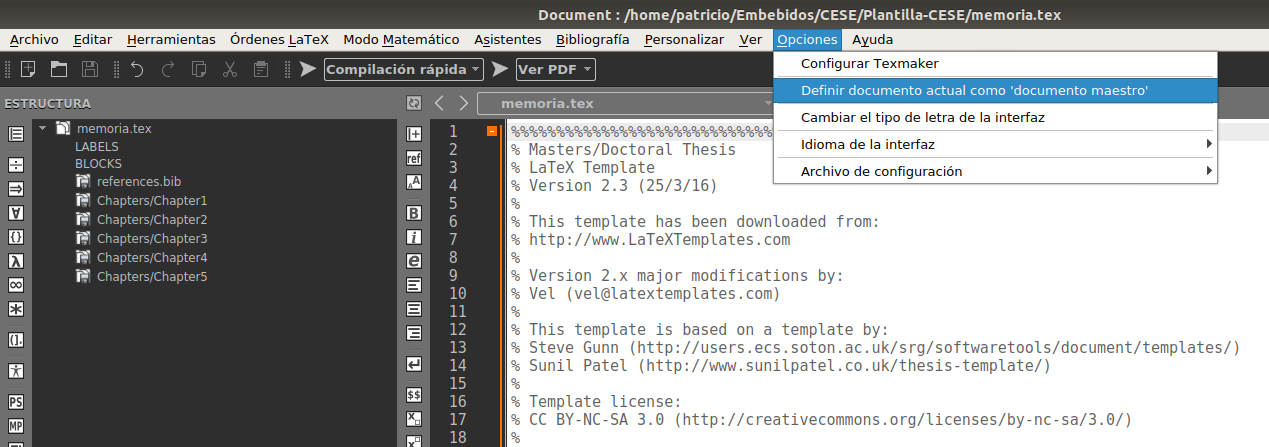
\includegraphics[width=\textwidth]{./Figures/docMaestro.png}
%	\caption{Definir memoria.tex como documento maestro.}
%	\label{fig:docMaestro}
%\end{figure}
%
%En el menú herramientas se encuentran las opciones de compilación.  Para producir un archivo PDF a partir de un archivo .tex se debe ejecutar PDFLaTeX (el shortcut es F6). Para incorporar nueva bibliografía se debe utilizar la opción BibTeX del mismo menú herramientas (el shortcut es F11).
%
%Notar que para actualizar las tablas de contenidos se debe ejecutar PDFLaTeX dos veces.  Esto se debe a que es necesario actualizar algunos archivos auxiliares antes de obtener el resultado final.  En forma similar, para actualizar las referencias se debe ejecutar primero PDFLaTeX, después BibTeX y finalmente PDFLaTeX dos veces por idénticos motivos.
%
%\section{Personalizando la plantilla, el archivo \file{memoria.tex}}
%\label{sec:FillingFile}
%
%Para personalizar la plantilla se debe incorporar la información propia en los distintos archivos \file{.tex}. 
%
%Primero abrir \file{memoria.tex} con TexMaker (o el editor de su preferencia). Se debe ubicar dentro del archivo el bloque de código titulado \emph{INFORMACIÓN DE LA PORTADA} donde se deben incorporar los primeros datos personales con los que se construirá automáticamente la portada.
%
%
%%----------------------------------------------------------------------------------------
%
%\section{El código del archivo \file{memoria.tex} explicado}
%
%El archivo \file{memoria.tex} contiene la estructura del documento y es el archivo de mayor jerarquía de la memoria.  Podría ser equiparable a la función \emph{main()} de un programa en C, o mejor dicho al archivo fuente .c donde se encuentra definida la función main().
%
%La estructura básica de cualquier documento de \LaTeX{} comienza con la definición de clase del documento, es seguida por un preámbulo donde se pueden agregar funcionalidades con el uso de \texttt{paquetes} (equiparables a bibliotecas de C), y finalmente, termina con el cuerpo del documento, donde irá el contenido de la memoria.
%
%\lstset{%
%  basicstyle=\small\ttfamily,
%  language=[LaTeX]{TeX}
%}
%
%\begin{lstlisting}
%\documentclass{article}  <- Definicion de clase
%\usepackage{listings}	 <- Preambulo
%
%\begin{document}	 <- Comienzo del contenido propio 
%	Hello world!
%\end{document}
%\end{lstlisting}
%
%
%El archivo \file{memoria.tex} se encuentra densamente comentado para explicar qué páginas, secciones y elementos de formato está creando el código \LaTeX{} en cada línea. El código está dividido en bloques con nombres en mayúsculas para que resulte evidente qué es lo que hace esa porción de código en particular. Inicialmente puede parecer que hay mucho código \LaTeX{}, pero es principalmente código para dar formato a la memoria por lo que no requiere intervención del usuario de la plantilla.  Sí se deben personalizar con su información los bloques indicados como:
%
%\begin{itemize}
%	\item Informacion de la memoria
%	\item Resumen
%	\item Agradecimientos
%	\item Dedicatoria
%\end{itemize}
%
%El índice de contenidos, las listas de figura de tablas se generan en forma automática y no requieren intervención ni edición manual por parte del usuario de la plantilla. 
%
%En la parte final del documento se encuentran los capítulos y los apéndices.  Por defecto se incluyen los 5 capítulos propuestos que se encuentran en la carpeta /Chapters. Cada capítulo se debe escribir en un archivo .tex separado y se debe poner en la carpeta \emph{Chapters} con el nombre \file{Chapter1}, \file{Chapter2}, etc\ldots El código para incluir capítulos desde archivos externos se muestra a continuación.
%
%\begin{verbatim}
%	% Chapter 1

\chapter{Introducción general} % Main chapter title

\label{Chapter1} % For referencing the chapter elsewhere, use \ref{Chapter1} 
\label{IntroGeneral}
Este capítulo introduce al lector sobre la necesidad de desarrollar un sistema que permita gestionar el recurso hídrico de manera eficiente en redes de canales. 
%----------------------------------------------------------------------------------------

% Define some commands to keep the formatting separated from the content 
\newcommand{\keyword}[1]{\textbf{#1}}
\newcommand{\tabhead}[1]{\textbf{#1}}
\newcommand{\code}[1]{\texttt{#1}}
\newcommand{\file}[1]{\texttt{\bfseries#1}}
\newcommand{\option}[1]{\texttt{\itshape#1}}
\newcommand{\grados}{$^{\circ}$}

%----------------------------------------------------------------------------------------

%\section{Introducción}

%----------------------------------------------------------------------------------------
\section{Descripción general}

La problemática del agua es central en el sostenimiento de los sistemas socioproductivos de distintas regiones de nuestro país. Las fuentes del vital recurso para la vida son escasas y en muchas circunstancias son aprovechadas de forma deficiente o bien el acceso a ellas se ve limitado por diversas causas. En este contexto, existen organismos tanto  públicos como privados que dan diagnósticos y resaltan dicha problemática de escasez, baja calidad y formas precarias de aprovechamiento de agua, muchas veces sin poder resolverla por cuestiones que tienen que ver con la disponibilidad de tecnologías apropiadas, la organización de la demanda y la gestión. 
 	 
En estas circunstancias, es posible reconocer situaciones cuando el recursos de agua es en abundancia, se puede entregar caudales mayores a los solicitados, asegurando agua a todos los usuarios, por lo que se puede identificar dos situaciones posibles, grandes pérdidas por derrames y baja eficiencia en la gestión del agua.

Actualmente son los operarios quienes recorren desde pocos hasta varios kilómetros y manualmente realizan las mediciones de los valores de parámetros necesarios con los que luego proceden a realizar el calculo correspondiente y establecer a la compuerta en una determinada posición y de esta manera fijar el caudal de agua deseado. 	 

Ante esta problemática, el propósito del presente proyecto es el diseño y construcción de un prototipo a escala de un sistema cuyo objetivo principal es suministrar una entrega eficiente de agua mediante la regulación de su caudal.

Como herramientas de trabajo, se aplicaron para la función de control, un algoritmo PID, como elemento actuador, se construyó una válvula de control servoalimentada, energizada por un motor paso a paso, y para la medición de la variable controlada, en este caso caudal, se construyó un caudalímetro por placa de aforo triangular, cuyas características dimensionales se determinaron en forma empírica.


%\subsection{Una introducción (no tan corta) a \LaTeX{}}
%
%Si sos nuevo en \LaTeX{}, hay un muy buen libro electrónico - disponible gratuitamente en Internet como un archivo PDF - llamado, \enquote{A (not so short) Introduction to \LaTeX{}}. El título del libro es generalmente acortado a simplemente \emph{lshort}. Puede descargar la versión más reciente en inglés (ya que se actualiza de vez en cuando) desde aquí:
%\url{http://www.ctan.org/tex-archive/info/lshort/english/lshort.pdf}
%
%Se puede encontrar la versión en español en la lista en esta página: \url{http://www.ctan.org/tex-archive/info/lshort/}
%
%\subsubsection{Una subsubsección}
%
%Acá tiene un ejemplo de una ``subsubsección'' que es el cuarto nivel de ordenamiento del texto, después de capítulo, sección y subsección.  Como se puede ver, las subsubsecciones no van numeradas en el cuerpo del documento ni en el índice.  El formato está definido por la plantilla y no debe ser modificado.
%
%\subsection{Guía matemática rápida para \LaTeX{}}
%
%Si estás escribiendo un documento con mucho contenido matemático, entonces es posible que desees leer el documento de la AMS (American Mathematical Society) llamado, \enquote{A Short Math Guide for \LaTeX{}}. Se puede encontrar en línea en el siguiente link: \url{http://www.ams.org/tex/amslatex.html} en la sección \enquote{Additional Documentation} hacia la parte inferior de la página.

%
%----------------------------------------------------------------------------------------

\section{Motivación}

La gestión de canales y redes de distribución de agua en la mayoría de las regiones del país se basa en operaciones de control manual en la que los operarios supervisan el estado de cada elemento y actúan en función de protocolos establecidos.
		
Hoy por hoy, estos procedimientos presentan una capacidad de reacción lenta ante la demanda variable de cada uno de los usuarios de agua,  ya que los operarios, en ocasiones deben recorrer varios kilómetros por lo que esto, representa un costo sumamente elevado mantener este servicio.

Este proyecto, además de regular el caudal de agua en canal abierto podrá resolver los problemas referentes a la disponibilidad de agua en regiones que presentan escasez por diferentes factores, no solo por sequías. Asimismo, no sólo busca maximizar la eficiencia en el abastecimiento de agua a cada uno de los usuarios en tiempo y forma, sino también minimizar la pérdida de la misma en la red de canales, y así, de esta manera, poder brindar mayor seguridad en el suministro de agua para el riego a cada productor en sus predios.

De este modo, se podrá obtener mejoras en la calidad de sus productos y por sobre todo, mayores rendimientos en su producción. El riego es la labor cultural que mayor impacto tiene sobre el rendimiento y la calidad en los productos. 

A fin de minimizar errores que introduce al trabajar con un prototipo formado por una compuerta esta fue reemplazada por una válvula, ya que de esta forma permite trabajar sin filtraciones de agua y mayor precisión en la medición.   	  
Es importante aclarar que una red o las redes de canales se encuentran separadas por compuertas. En el prototipo la válvula simula ser una compuerta.

Uno de los objetivos planteados para una segunda fase de desarrollo es instanciar, este sistema desarrollado en el presente informe, en varias compuertas que constituye una red de canal de modo tal, que las mismas se comuniquen entre sí utilizando tecnología LoraWan y lograr como sistema general se ejecute de forma autónoma.  

Con el presente sistema de control también se busca promover la recuperación del potencial productivo de los suelos agropecuarios  que se han degradado por diferentes factores, entre ellos la escasez de agua. 

Es de destacar que no existen soluciones nacionales, por lo tanto,  el desafío es lograr ser competitivo en precio y prestaciones con productos importados que se encuentran en el mercado. Esto trae aparejado, desde el punto vista del cliente el beneficio de contar con soporte local y la posibilidad de modificar algo del sistema según las necesidades del cliente.

%----------------------------------------------------------------------------------------

\section{Objetivos y alcances}

%\subsection{Objetivos}

El objetivo general de este trabajo es aportar el diseño y elaboración de un sistema que mediante el empleo de un algoritmo de control PID permite regular el caudal de agua en canal abierto y con el uso de las tecnologías más actuales pueda ser empleado tanto en red de canales complejos hasta las redes más simples. A continuación se detallan los subobjetivos específicos que se tuvieron en cuenta :  
\begin{itemize}
\item Diseño y construcción de  un sistema de control que permita al usuario establecer un caudal de agua determinado de forma remota.

\item Diseño y fabricación de un circuito de control de señales cuya finalidad del mismo es cumplir la función de interfaz entre la etapa de control y la de potencia correspondiente al driver del motor paso a paso. 
\item El firmware incluye un sistema de tiempo real.  
\item Para regular el caudal de agua, aplicar un algoritmo de control PID.
\item Empleo de un sensor de presión que posea una precisión de 1 mm para detectar el nivel de la superficie del agua.
\item Utilización de un potenciómetro de manera tal que conjuntamente a un motor paso a paso conformen un servo motor y posicionar a la válvula en un determinado ángulo.  
\item Proporcionar una gestión de agua de riego de forma eficiente.
\item Desarrollar un firmware escalable de tal modo que permita la comunicación con otros firmware's instanciados en otras compuerta. 
\end{itemize}

 
%Esta plantilla se distribuye como una único archivo .zip que se puede descomprimir en varios archivos y carpetas. Asimismo, se puede consultar el repositorio git para obtener la última versión de los archivos, \url{https://github.com/patriciobos/Plantilla-CESE.git}. Los nombres de las carpetas son, o pretender ser, auto-explicativos.
%
%\keyword{Appendices} -- Esta es la carpeta donde se deben poner los apéndices. Cada apéndice debe ir en su propio archivo \file{.tex}. Se incluye un ejemplo y una plantilla en la carpeta.
%
%\keyword{Chapters} -- Esta es la carpeta donde se deben poner los capítulos de la memoria. Cada capítulo debe ir un su propio archivo \file{.tex} por separado.  Se ofrece por defecto, la siguiente estructura de capítulos y se recomienda su utilización dentro de lo posible:
%
%\begin{itemize}
%\item Capítulo 1: Introducción general	
%\item Capítulo 2: Introducción específica
%\item Capítulo 3: Diseño e implementación
%\item Capítulo 4: Ensayos y resultados
%\item Capítulo 5: Conclusiones
%
%\end{itemize}
%
%Esta estructura de capítulos es la que se recomienda para las memorias de la especialización.
%
%\keyword{Figures} -- Esta carpeta contiene todas las figuras de la memoria.  Estas son las versiones finales de las imágenes que van a ser incluidas en la memoria.  Pueden ser imágenes en formato \textit{raster}\footnote{\url{https://en.wikipedia.org/wiki/Raster_graphics}} como \file{.png}, \file{.jpg} o en formato vectoriales\footnote{\url{https://en.wikipedia.org/wiki/Vector_graphics}} como \file{.pdf}, \file{.ps}.  Se debe notar que utilizar imágenes vectoriales disminuye notablemente el peso del documento final y acelera el tiempo de compilación por lo que es recomendable su utilización siempre que sea posible.
%
%\subsection{Archivos}
%
%También están incluidos varios archivos, la mayoría de ellos son de texto plano y se puede ver su contenido en un editor de texto. Después de la compilación inicial, se verá que más archivos auxiliares son creados por \ LaTeX{} o BibTeX, pero son de uso interno y no es necesario hacer nada en particular con ellos.  Toda la información necesaria para compilar el documento se encuentra en los archivos \file{.tex}, \file{.bib}, \file{.cls} y en las imágenes de la carpeta Figures.
%
%\keyword{referencias.bib} - este es un archivo importante que contiene toda la información de referencias bibliográficas que se utilizarán para las citas en la memoria en conjunto con BibTeX. Usted puede escribir las entradas bibliográficas en forma manual, aunque existen también programas de gestión de referencias que facilitan la creación y gestión de las referencias y permiten exportarlas en formato BibTeX.  También hay disponibles sitios web como \url{books.google.com} que permiten obtener toda la información necesaria para una cita en formato BibTeX. Ver sección \ref{sec:biblio}
%
%\keyword{MastersDoctoralThesis.cls} -- este es un archivo importante. Es el archivos con la clase que le informa a \LaTeX{} cómo debe dar formato a la memoria. El usuario de la plantilla no debería necesitar modificar nada de este archivo.
%
%\keyword{memoria.pdf} -- esta es su memoria con una tipografía bellamente compuesta (en formato de archivo PDF) creado por \LaTeX{}. Se distribuye con la plantilla y después de compilar por primera vez sin hacer ningún cambio se debería obtener una versión idéntica a este documento.
%
%\keyword{memoria.tex} -- este es un archivo importante. Este es el archivo que tiene que compilar \LaTeX{} para producir la memoria como un archivo PDF. Contiene un marco de trabajo y estructuras que le indican a \LaTeX{} cómo diagramar la memoria.  Está altamente comentado para que se pueda entender qué es lo que realiza cada línea de código y por qué está incluida en ese lugar.  En este archivo se debe completar la información personalizada de las primeras sección según se indica en la sección \ref{sec:FillingFile}.
%
%Archivos que \emph{no} forman parte de la distribución de la plantilla pero que son generados por \LaTeX{} como archivos auxiliares necesarios para la producción de la memoria.pdf son:
%
%\keyword{memoria.aux} -- este es un archivo auxiliar generado por \LaTeX{}, si se borra \LaTeX{} simplemente lo regenera cuando se compila el archivo principal \file{memoria.tex}.
%
%\keyword{memoria.bbl} -- este es un archivo auxiliar generado por BibTeX, si se borra BibTeX simplemente lo regenera cuando se compila el archivo principal \file{memoria.tex}. Mientras que el archivo \file{.bib} contiene todas las referencias que hay, este archivo \file{.bbl} contine sólo las referencias que han sido citadas y se utiliza para la construcción de la bibiografía.
%
%\keyword{memoria.blg} -- este es un archivo auxiliar generado por BibTeX, si se borra BibTeX simplemente lo regenera cuando se compila el archivo principal \file{memoria.tex}.
%
%\keyword{memoria.lof} -- este es un archivo auxiliar generado por \LaTeX{}, si se borra \LaTeX{} simplemente lo regenera cuando se compila el archivo principal \file{memoria.tex}.  Le indica a \LaTeX{} cómo construir la sección \emph{Lista de Figuras}.
% 
%\keyword{memoria.log} --  este es un archivo auxiliar generado por \LaTeX{}, si se borra \LaTeX{} simplemente lo regenera cuando se compila el archivo principal \file{memoria.tex}. Contiene mensajes de \LaTeX{}. Si se reciben errores o advertencias durante la compilación, se guardan en este archivo \file{.log}.
%
%\keyword{memoria.lot} -- este es un archivo auxiliar generado por \LaTeX{}, si se borra \LaTeX{} simplemente lo regenera cuando se compila el archivo principal \file{memoria.tex}.  Le indica a \LaTeX{} cómo construir la sección \emph{Lista de Tablas}.
%
%\keyword{memoria.out} -- este es un archivo auxiliar generado por \LaTeX{}, si se borra \LaTeX{} simplemente lo regenera cuando se compila el archivo principal \file{memoria.tex}.
%
%De esta larga lista de archivos, sólo aquellos con la extensión \file{.bib}, \file{.cls} y \file{.tex} son importantes.  Los otros archivos auxiliares pueden ser ignorados o borrados ya que \LaTeX{} y BibTeX los regenerarán durante la compilación.
%
%%----------------------------------------------------------------------------------------
%
%\section{Entorno de trabajo}
%
%Ante de comenzar a editar la plantilla debemos tener un editor \LaTeX{} instalado en nuestra computadora.  En forma análoga a lo que sucede en lenguaje C, que se puede crear y editar código con casi cualquier editor, existen ciertos entornos de trabajo que nos pueden simplificar mucho la tarea.  En este sentido, se recomienda, sobre todo para los principiantes en \LaTeX{} la utilización de TexMaker, un programa gratuito y multi-plantaforma que está disponible tanto para windows como para sistemas GNU/linux.
%
%La versión más reciente de TexMaker es la 4.5 y se puede descargar del siguiente link: \url{http://www.xm1math.net/texmaker/download.html}. Se puede consultar el manual de usuario en el siguiente link: \url{http://www.xm1math.net/texmaker/doc.html}.
% 
%
%\subsection{Paquetes adicionales}
%
%Si bien durante el proceso de instalación de TexMaker, o cualquier otro editor que se haya elegido, se instalarán en el sistema los paquetes básicos necesarios para trabajar con \LaTeX{}, la plantilla de los trabajos de Especialización y Maestría requieren de paquete adicionales.
%
%Se indican a continuación los comandos que se deben introducir en la consola de Ubuntu (ctrl + alt + t) para instalarlos:
%
%\begin{lstlisting}[language=bash]
%  $ sudo apt install texlive-lang-spanish texlive-science 
%  $ sudo apt install texlive-bibtex-extra biber
%  $ sudo apt install texlive texlive-fonts-recommended
%  $ sudo apt install texlive-latex-extra
%\end{lstlisting}
%
%
%\subsection{Configurando TexMaker}
%
%
%Una vez instalado el programa y los paquetes adicionales se debe abrir el archivo memoria.tex con el editor para ver una pantalla similar a la que se puede apreciar en la figura \ref{fig:texmaker}. 
%
%\begin{figure}[h]
%	\centering
%	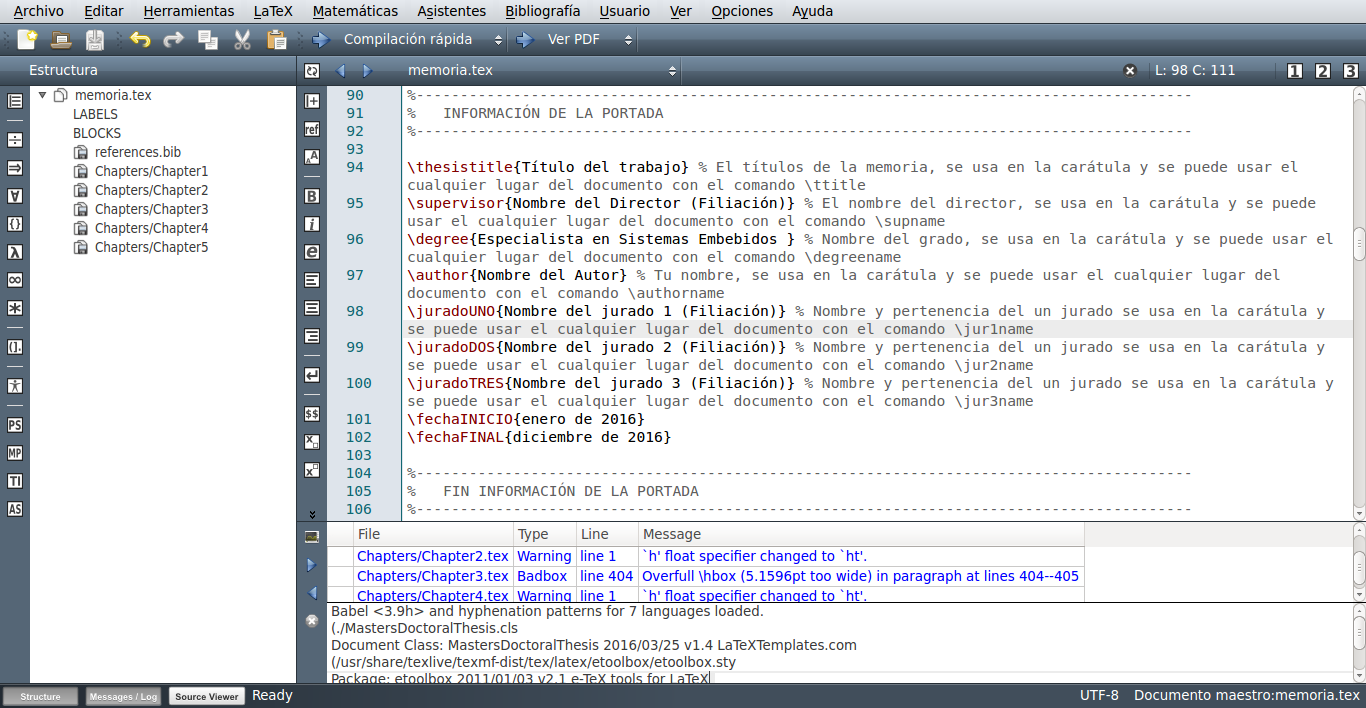
\includegraphics[width=\textwidth]{./Figures/texmaker.png}
%	\caption{Entorno de trabajo de texMaker.}
%	\label{fig:texmaker}
%\end{figure}
%
%Notar que existe una vista llamada Estructura a la izquierda de la interfaz que nos permite abrir desde dentro del programa los archivos individuales de los capítulos.  A la derecha se encuentra una vista con el archivo propiamente dicho para su edición. Hacia la parte inferior se encuentra una vista del log con información de los resultados de la compilación.  En esta última vista pueden aparecen advertencias o \textit{warning}, que normalmente pueden ser ignorados, y los errores que se indican en color rojo y deben resolverse para que se genere el PDF de salida.
%
%Recordar que el archivo que se debe compilar con PDFLaTeX es \file{memoria.tex}, si se tratara de compilar alguno de los capítulos saldría un error.  Para salvar la molestia de tener que cambiar de archivo para compilar cada vez que se realice una modificación en un capítulo, se puede definir el archivo \file{memoria.tex} como ``documento maestro'' yendo al menú opciones -> ``definir documento actual como documento maestro'', lo que permite compilar con PDFLaTeX memoria.tex directamente desde cualquier archivo que se esté modificando . Se muestra esta opción en la figura \ref{fig:docMaestro}.
%
%\begin{figure}[h]
%	\centering
%	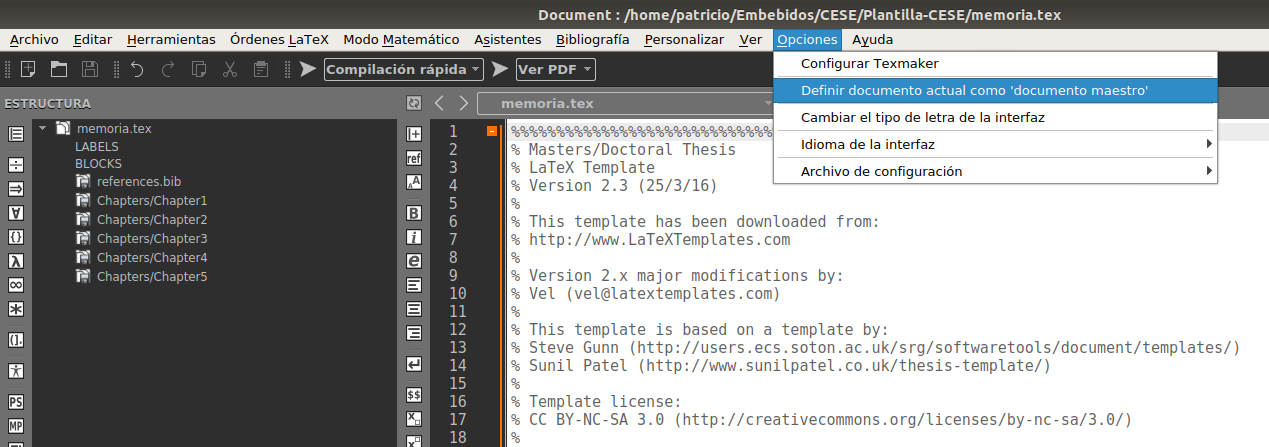
\includegraphics[width=\textwidth]{./Figures/docMaestro.png}
%	\caption{Definir memoria.tex como documento maestro.}
%	\label{fig:docMaestro}
%\end{figure}
%
%En el menú herramientas se encuentran las opciones de compilación.  Para producir un archivo PDF a partir de un archivo .tex se debe ejecutar PDFLaTeX (el shortcut es F6). Para incorporar nueva bibliografía se debe utilizar la opción BibTeX del mismo menú herramientas (el shortcut es F11).
%
%Notar que para actualizar las tablas de contenidos se debe ejecutar PDFLaTeX dos veces.  Esto se debe a que es necesario actualizar algunos archivos auxiliares antes de obtener el resultado final.  En forma similar, para actualizar las referencias se debe ejecutar primero PDFLaTeX, después BibTeX y finalmente PDFLaTeX dos veces por idénticos motivos.
%
%\section{Personalizando la plantilla, el archivo \file{memoria.tex}}
%\label{sec:FillingFile}
%
%Para personalizar la plantilla se debe incorporar la información propia en los distintos archivos \file{.tex}. 
%
%Primero abrir \file{memoria.tex} con TexMaker (o el editor de su preferencia). Se debe ubicar dentro del archivo el bloque de código titulado \emph{INFORMACIÓN DE LA PORTADA} donde se deben incorporar los primeros datos personales con los que se construirá automáticamente la portada.
%
%
%%----------------------------------------------------------------------------------------
%
%\section{El código del archivo \file{memoria.tex} explicado}
%
%El archivo \file{memoria.tex} contiene la estructura del documento y es el archivo de mayor jerarquía de la memoria.  Podría ser equiparable a la función \emph{main()} de un programa en C, o mejor dicho al archivo fuente .c donde se encuentra definida la función main().
%
%La estructura básica de cualquier documento de \LaTeX{} comienza con la definición de clase del documento, es seguida por un preámbulo donde se pueden agregar funcionalidades con el uso de \texttt{paquetes} (equiparables a bibliotecas de C), y finalmente, termina con el cuerpo del documento, donde irá el contenido de la memoria.
%
%\lstset{%
%  basicstyle=\small\ttfamily,
%  language=[LaTeX]{TeX}
%}
%
%\begin{lstlisting}
%\documentclass{article}  <- Definicion de clase
%\usepackage{listings}	 <- Preambulo
%
%\begin{document}	 <- Comienzo del contenido propio 
%	Hello world!
%\end{document}
%\end{lstlisting}
%
%
%El archivo \file{memoria.tex} se encuentra densamente comentado para explicar qué páginas, secciones y elementos de formato está creando el código \LaTeX{} en cada línea. El código está dividido en bloques con nombres en mayúsculas para que resulte evidente qué es lo que hace esa porción de código en particular. Inicialmente puede parecer que hay mucho código \LaTeX{}, pero es principalmente código para dar formato a la memoria por lo que no requiere intervención del usuario de la plantilla.  Sí se deben personalizar con su información los bloques indicados como:
%
%\begin{itemize}
%	\item Informacion de la memoria
%	\item Resumen
%	\item Agradecimientos
%	\item Dedicatoria
%\end{itemize}
%
%El índice de contenidos, las listas de figura de tablas se generan en forma automática y no requieren intervención ni edición manual por parte del usuario de la plantilla. 
%
%En la parte final del documento se encuentran los capítulos y los apéndices.  Por defecto se incluyen los 5 capítulos propuestos que se encuentran en la carpeta /Chapters. Cada capítulo se debe escribir en un archivo .tex separado y se debe poner en la carpeta \emph{Chapters} con el nombre \file{Chapter1}, \file{Chapter2}, etc\ldots El código para incluir capítulos desde archivos externos se muestra a continuación.
%
%\begin{verbatim}
%	\include{Chapters/Chapter1}
%	\include{Chapters/Chapter2} 
%	\include{Chapters/Chapter3}
%	\include{Chapters/Chapter4} 
%	\include{Chapters/Chapter5} 
%\end{verbatim}
%
%Los apéndices también deben escribirse en archivos .tex separados, que se deben ubicar dentro de la carpeta \emph{Appendices}. Los apéndices vienen comentados por defecto con el caracter \code{\%} y para incluirlos simplemente se debe eliminar dicho caracter.
%
%Finalmente, se encuentra el código para incluir la bibliografía en el documento final.  Este código tampoco debe modificarse. La metodología para trabajar las referencias bibliográficas se desarrolla en la sección \ref{sec:biblio}.
%%----------------------------------------------------------------------------------------
%
%\section{Bibliografía}
%\label{sec:biblio}
%
%Las opciones de formato de la bibliografía se controlan a través del paquete de latex \option{biblatex} que se incluye en la memoria en el archivo memoria.tex.  Estas opciones determinan cómo se generan las citas bibliográficas en el cuerpo del documento y cómo se genera la bibliografía al final de la memoria.
%
%En el preámbulo se puede encontrar el código que incluye el paquete biblatex, que no requiere ninguna modificación del usuario de la plantilla, y que contiene las siguientes opciones:
%
%\begin{lstlisting}
%\usepackage[backend=bibtex,
%	natbib=true, 
%	style=numeric, 
%	sorting=none]
%{biblatex}
%\end{lstlisting}
%
%En el archivo \file{reference.bib} se encuentran las referencias bibliográficas que se pueden citar en el documento.  Para incorporar una nueva cita al documento lo primero es agregarla en este archivo con todos los campos necesario.  Todas las entradas bibliográficas comienzan con $@$ y una palabra que define el formato de la entrada.  Para cada formato existen campos obligatorios que deben completarse. No importa el orden en que las entradas estén definidas en el archivo .bib.  Tampoco es importante el orden en que estén definidos los campos de una entrada bibliográfica. A continuación se muestran algunos ejemplos:
%
%\begin{lstlisting}
%@ARTICLE{ARTICLE:1,
%    AUTHOR="John Doe",
%    TITLE="Title",
%    JOURNAL="Journal",
%    YEAR="2017",
%}
%\end{lstlisting}
%
%
%\begin{lstlisting}
%@BOOK{BOOK:1,
%    AUTHOR="John Doe",
%    TITLE="The Book without Title",
%    PUBLISHER="Dummy Publisher",
%    YEAR="2100",
%}
%\end{lstlisting}
%
%
%\begin{lstlisting}
%@INBOOK{BOOK:2,
%    AUTHOR="John Doe",
%    TITLE="The Book without Title",
%    PUBLISHER="Dummy Publisher",
%    YEAR="2100",
%    PAGES="100-200",
%}
%\end{lstlisting}
%
%
%\begin{lstlisting}
%@MISC{WEBSITE:1,
%    HOWPUBLISHED = "\url{http://example.com}",
%    AUTHOR = "Intel",
%    TITLE = "Example Website",
%    MONTH = "12",
%    YEAR = "1988",
%    URLDATE = {2012-11-26}
%}
%\end{lstlisting}
%
%Se debe notar que los nombres \emph{ARTICLE:1}, \emph{BOOK:1}, \emph{BOOK:2} y \emph{WEBSITE:1} son nombres de fantasía que le sirve al autor del documento para identificar la entrada. En este sentido, se podrían reemplazar por cualquier otro nombre.  Tampoco es necesario poner : seguido de un número, en los ejemplos sólo se incluye como un posible estilo para identificar las entradas.
%
%La entradas se citan en el documento con el comando: 
%
%\begin{verbatim}
%\citep{nombre_de_la_entrada}
%\end{verbatim}
%
%Y cuando se usan, se muestran así: \citep{ARTICLE:1}, \citep{BOOK:1}, \citep{BOOK:2}, \citep{WEBSITE:1}.  Notar cómo se conforma la sección Bibliografía al final del documento. 

%	\chapter{Introducción específica} % Main chapter title

\label{Chapter2}

%----------------------------------------------------------------------------------------
%	SECTION 1
%----------------------------------------------------------------------------------------
%Todos los capítulos deben comenzar con un breve párrafo introductorio que indique cuál es el contenido que se encontrará al leerlo.  La redacción sobre el contenido de la memoria debe hacerse en presente y todo lo referido al proyecto en pasado, siempre de modo impersonal.
En este capítulo se abordarán temas referentes al análisis de la estructura del sistema que se desarrolló, gestión, planificación del trabajo y técnicas relacionadas al sensor empleado.  	 

\section{Estructura general del sistema}
\label{sec:estructgeneralsistema}

%\subsection{Uso de mayúscula inicial para los título de secciones}

%Si en el texto se hace alusión a diferentes partes del trabajo referirse a ellas como capítulo, sección o subsección según corresponda. Por ejemplo: ``En el capítulo \ref{Chapter1} se explica tal cosa'', o ``En la sección \ref{sec:ejemplo} se presenta lo que sea'', o ``En la subsección \ref{subsec:ejemplo} se discute otra cosa''.
 
En un plano para la construcción del prototipo a escala, se pudo reconocer un inconveniente. Al emplear una compuerta que se desplaza verticalmente y ubicada en forma perpendicular al canal, se generarían filtraciones de agua en sus guías de desplazamiento. Como se trata de una maqueta a escala, estas filtraciones provocarían errores considerables al momento de realizar las mediciones relacionadas con la altura de la superficie de agua, y cálculos pertinentes al aplicar el método de aforo por compuerta para determinar el caudal. Por lo tanto, en el sistema no se obtendrían los resultados esperados. En este contexto, el caudal que circularía por debajo de la compuerta sería menor que el que se registraría en el caudalímetro. De esta forma, se obtendrían dos valores de caudales diferentes debido, entre otros factores, a las filtraciones.     
Esto motivó a reemplazar, en el prototipo, la compuerta por una válvula y así eliminar los errores que introducen dichas filtraciones. 
Para el control de la válvula se elaboró un servomotor con el empleo de un motor paso a paso con su correspondiente controlador.
En la figura \ref{fig:Vertedero triangular}, se puede apreciar un vertedero triangular en un canal abierto y una regla que mide el nivel de la superficie de agua.
\begin{figure}[h]
\centering
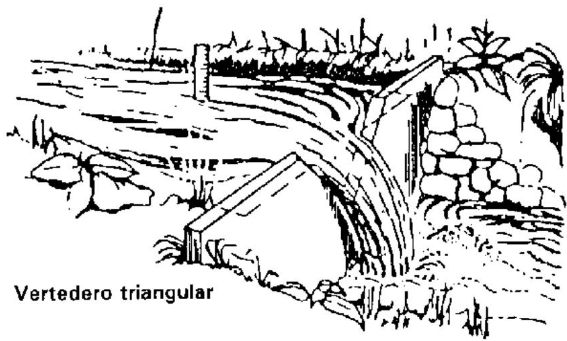
\includegraphics[scale=.60]{./Figures/VertederoTriangular.png}
\caption{Ilustración de un vertedero triangular ubicado en determinado punto a medir caudal en el canal.}
\label{fig:Vertedero triangular}
\end{figure}

Para medir el caudal, se fabricó un caudalímetro por placa de aforo triangular. Estos tipos de instrumentos, también denominados vertederos, representan un dique o pared que intercepta en un determinado punto una corriente de líquido, en este caso agua, con superficie libre, como se puede apreciar en la figura 2.1 . En general, se utilizan para mantener un nivel de superficie de aguas arriba que no exceda de un valor límite, o bien para medir el caudal de agua circulante por un canal. Este instrumento resulta un medidor de caudal sencillo pero efectivo en canales abiertos. 

El principio de funcionamiento de la celda primaria consiste en establecer el caudal de agua a un valor establecido por el usuario. Para llevar a cabo esto, fue necesario el desarrollo de un firmware que controla el eje de un servomotor. Este se encuentra adherido a una válvula, lo que permite maniobrar su rango de apertura para regular el flujo del fluido según las necesidades.

El diagrama de control correspondiente es el que se muestra en la figura \ref{fig:CeldaPrimaria} donde se aprecia que la salida del servomotor actúa directamente sobre la válvula. Esta puede ser una llave esférica, como es este el caso, o un sistema de cremallera. Este tipo de sistemas se aplican a compuertas verticales, como las que podemos encontrar frecuentemente en los canales de agua a cielo abierto. La salida de la válvula es el flujo controlado de caudal al canal. En este punto se coloca un medidor de caudal. Luego su resultado se compara con el set point, valor de caudal fijado por el usuario. En el sumador, a partir de la diferencia que existe entre el set point y el valor de caudal medido se obtiene una señal de error, que seguidamente se procesa por un algoritmo de control PID para que sea igual a cero.

\begin{figure}[htpb]
\centering
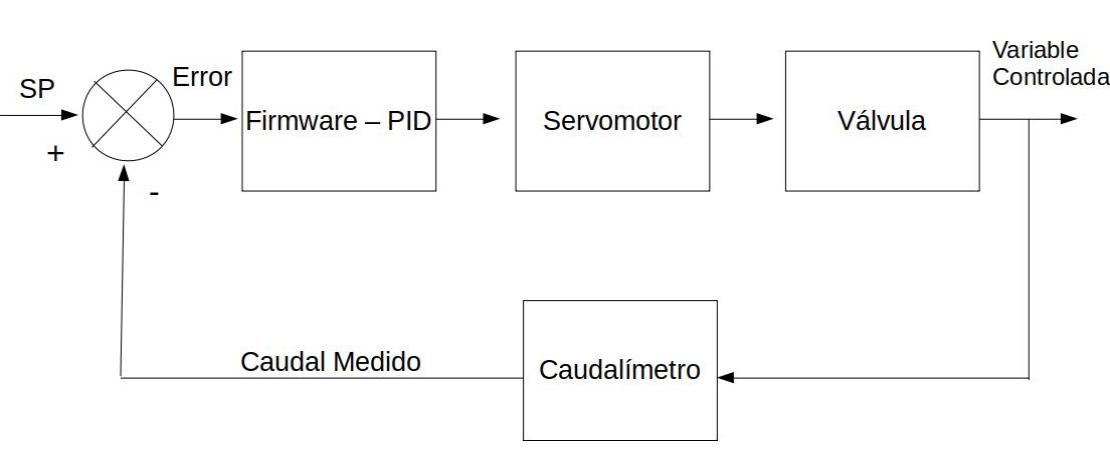
\includegraphics[scale=.45]{./Figures/DiagramaEnBloqueDeControlCeldaPrimaria-V5.png}
\caption{Diagrama en bloque de control - celda primaria.}
\label{fig:CeldaPrimaria}
\end{figure}

\section{Compuertas Miller}
\label{sec:Compuertas miller}
Las compuertas Miller es el mecanismo más utilizado en los canales de agua de riego para controlar la entrada de agua de los canales ramales y tomas directas a las parcelas. Están construidas de fierro fundido (vaciado o colado) por su resistencia a la oxidación. Sin embargo, son frágiles y poco maleables. La toma Miller, en esencia, es una compuerta circular que obtura la entrada a la tubería de salida, la que es izada por un mecanismo elevador compuesto de un vástago cilíndrico con cuerda tipo tornillo (roscas), generalmente de 2” de diámetro y longitud variable, en función de la altura a colocar la toma y un volante. Las tomas-granja Miller se clasifican por el diámetro de la tubería a obturar, y son de 18” y 24” las más comunes para tomas-granjas, mientras que las de 30” y 36” son usadas para abastecer ramales y subramales.
Las ventajas de este tipo de tomas es que son relativamente baratas, la mayoría de las fundidoras las pueden construir y son de fácil colocación. Como desventajas, destacan que pueden tener filtraciones de consideración al ser difícil un cierre hermético debido al metal de la tubería y de la compuerta (comal), especialmente si, durante su fundición, no hay cuidado de tener acabados completamente a nivel. La calibración de esta estructura es difícil, ya que al abrirse parcialmente la compuerta sobre la tubería ambas de figura circular, se forman secciones tipo “media luna” con área hidráulica variable, sin seguir un patrón de fácil cálculo. 
En las figuras \ref{fig:Compuerta tipo miller para toma-granja}, \ref{fig:Conducto preparado para colocar compuerta tipo miller.} y \ref{fig:Toma granja tipo miller de compuerta circular.} se puede apreciar como es la estructura de la compuerta, el conducto para la toma y su colocación.

\begin{figure}[h]
\centering
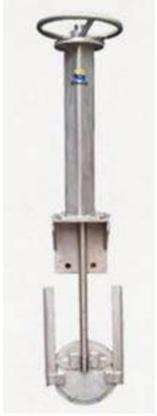
\includegraphics[scale=.65]{./Figures/CompuertaMiller.jpeg}
\caption{Compuerta tipo Miller para toma-granja.}
\label{fig:Compuerta tipo miller para toma-granja}
\end{figure}

\begin{figure}[h]
\centering
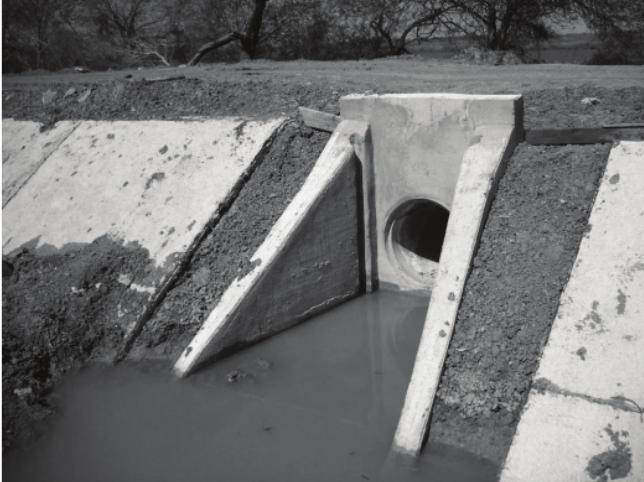
\includegraphics[scale=.58]{./Figures/ConductoPreparadoParaCompuertaMiller.jpeg}
\caption{Conducto preparado para colocar compuerta tipo Miller.}
\label{fig:Conducto preparado para colocar compuerta tipo miller.}
\end{figure}


\begin{figure}[htpb]
\centering
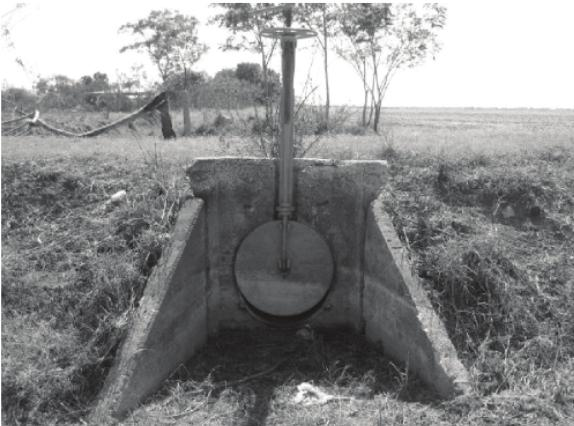
\includegraphics[scale=.65]{./Figures/compuertamillercircular.jpeg}
\caption{Toma-granja tipo Miller de compuerta circular de 18” de diámetro.}
\label{fig:Toma granja tipo miller de compuerta circular.}
\end{figure}

Este mecanismo que se mostró y que se emplea en muchos países para el control de entrada de agua a los canales principales o bien a las parcelas, impulsó a utilizar, en el prototipo a escala, una válvula esférica simulando ser una compuerta Miller.   

\section{Requerimiento a nivel de software y hardware}
\label{sec:ejemplo}
En esta sección se presentan los requerimientos específicos de software y hardware del sistema. Estos se tuvieron en cuenta al momento de inicio del desarrollo de este proyecto, cuyo fin es, mediante el control de movimiento de una válvula regular el caudal de agua según las necesidades del usuario. 
\subsection{Requisitos específicos del software}
\label{subsec:ejemplo}


 Los requisitos específicos de software fueron:

\begin{enumerate}
	\item El firmware deberá generar como señal, trenes de pulsos para controlar el movimiento del eje perteneciente al servomotor.
	\item El firmware deberá determinar, mediante el sensor de presión en conjunto con la placa de aforo triangular, el caudal de agua que fluye a través de este instrumento de medición.
	\item  El firmware deberá incluir un algoritmo de control PID, que por medio de un lazo de retroalimentación permitiese regular la variable a controlar.
	\item El firmware deberá ser capaz, a través de un pin configurado como salida, establecer el sentido de giro del eje del servomotor, horario - antihorario.
	\item El firmware deberá ser capaz, a través de un pin configurado como salida, habilitar - deshabilitar el servomotor.
	\item El firmware deberá interactuar, mediante el empleo del puerto serial, con otra aplicación. 	  
	\item Con un protocolo de comunicación definido entre la aplicación externa y el firmware, este último deberá ser capaz de recibir y enviar datos.
	\item El firmware deberá enviar una notificación de correcta recepción de cualquier comando mediante el envío de un comando específico hacía la aplicación externa.  
	\item El firmware deberá reportar o notificar a la aplicación externa la recepción de un comando inválido mediante un comando específico.
	\item En caso de recepción de comandos válidos, el firmware deberá informar internamente que hay datos a procesar. 
\end{enumerate}

\subsection{Requisitos específicos del hardware}
\label{subsec:requisitoshw}
 Los requisitos específicos principales de hardware fueron:
\begin{enumerate}
	\item Se hará uso de la placa EDU-CIAA-NXP como computadora principal para el prototipo a escala.
	\item Se construirá un mecanizado de  válvula de control estándar mediante un servomotor energizado paso a paso y un elemento medidor de ángulo tipo potenciométrico resistivo.
	\item Se construirá un medidor de caudal por canal de aforo utilizando para la medición de la altura de nivel de agua un sensor MPX5010DP.
	\item Se diseñará y fabricará un circuito como interfaz que controlará las señales enviadas desde la placa EDU-CIAA-NXP al controlador del servomotor paso a paso. 
\end{enumerate}

\section{Características de hardware propias del equipo}
\label{sec:Características propias del equipo}
\subsection{Motor paso a paso y controlador}
Para la construcción de la válvula de control fue preciso emplear un motor  que tenga la capacidad de mover una llave esférica. Para este proyecto, por cuestión de disponibilidad, se utilizó un motor paso a paso y un controlador cuyo modelos son 86HS85 y MA860H respectivamente.
El motor paso a paso de 8 hilos posee un torque nominal de 8,5 Nm, suficiente como para realizar movimientos de apertura parcial o total y cierre total de la carrera de una válvula, según las necesidades requeridas de caudal. 
El driver MA860H es un controlador para motores paso a paso compatibles con motores 86HS85 con las siguientes características principales:

\begin{enumerate}
	\item Permite ajustar la corriente que se dirige hacia el motor.
	\item Posibilita controlar al motor hasta en 200 micropasos.
	\item Frecuencia de entrada de tren de pulso hasta 300 khz. 
	\item Corriente de salida hasta 7.2A.
	\item Entrada TTL compatible y ópticamente aislada.
	\item Soporta modos PUL / DIR y CW / CCW.
\end{enumerate}

El MA860H tiene dos conectores, el conector P1 para conexiones de señales de control y el conector P2 para conexiones de potencia y motor.     
Para el control de la válvula fue necesario un motor que pueda producir un momento de 1 Nm o más. 

\subsubsection{Configuraciones del conector P1}
\begin{itemize}

\item Señal de pulso: esta entrada representa la señal de pulso, activa en cada flanco ascendente o descendente (para este trabajo se encuentra configurado en flanco ascendente). Entre 4V y 5V equivale a un pulso alto, entre 0V y 5V a un pulso bajo. Para una respuesta confiable, el ancho de pulso debe ser superior a 1,5 uS. 

\item Señal de dirección: esta señal tiene niveles de voltaje bajo y alto, que representan dos direcciones de rotación del motor. Para una respuesta de movimiento confiable, la señal de dirección debe estar por delante de la señal de pulso por lo menos 5 uS. Entre 4V y 5V equivale a un pulso alto, entre 0V y 5V a un pulso bajo.

\item Señal de habilitación: esta señal se utiliza para habilitar/deshabilitar el controlador. Nivel alto para habilitar y nivel bajo para inhabilitar al controlador.

\end{itemize}
\subsection{Sensor de presión}
Para monitorizar el nivel de la columna de agua, necesario para determinar el caudal en un determinado instante, se optó por su alta precisión un sensor de presión cuyo modelo es MPX5010DP. Este transductor piezo-resistivo, es un sensor de presión de silicio monolítico que puede ser utilizado en aplicaciones que disponen de un microcontrolador o microprocesador con entradas ADC.
El MPX5010DP entrega a su salida un rango de voltaje entre 0V y 5V, mediante esta información y una fórmula que se expone en el siguiente párrafo se puede estimar la presión hasta un valor de 10 KPa, esto es, una columna de agua de hasta 100 cm de altura.
El dispositivo proporciona una salida lineal como puede se observar en la figura \ref{fig:función de salida del sensor}, extraída de su hoja de datos.

\begin{figure}[h]
\centering
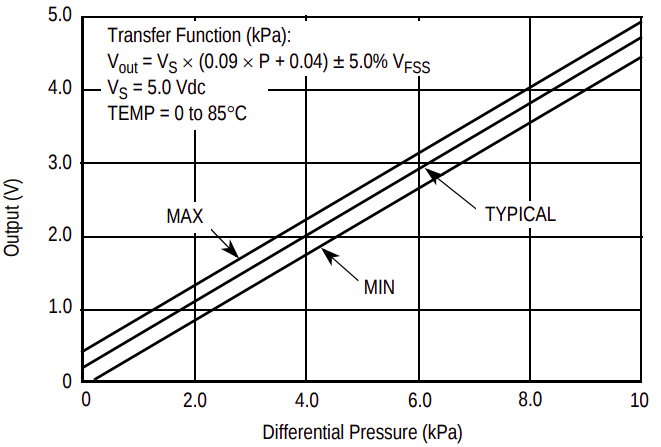
\includegraphics[scale=.55]{./Figures/SalidaMPX5010DP.png}
\caption{Función de salida del sensor de presión MPX5010DP.}
\label{fig:función de salida del sensor}
\end{figure}
Como se pudo observar la función de la figura \ref{fig:función de salida del sensor}, la ecuación para obtener la presión del sensor viene dada por la ecuación \ref{eq:presion}:

\begin{equation}
 \label{eq:presion}
 P = \frac{Vout- 0.04*Vs \pm Tol}{0.09*Vs}
\end{equation}

\vspace{3cm}
Donde:\\
\begin{itemize}
\item Vs: es el valor de voltaje de alimentación, Vs = 5V.\\
\item Vout: es el valor de voltaje que entrega el sensor  a su salida.\\
\item Tol: es la tolerancia, un ajuste que se debe aplicar al sensor para  calibrar a medida.
\end{itemize}

Tomando como base la ecuación de presión diferencial que relaciona la altura se resuelve que (recordando que a la presión atmosférica normal es cero):  

\begin{equation}
 \label{eq:presiónII}
	 P =PH -PL= P = \rho gh =\frac{Vout- 0.04*Vs \pm Tol}{0.09*Vs}	
\end{equation}
 Donde:
 \begin{itemize}
 \item P: es la presión.
 \item $\rho$: es la densidad del agua.
 \item g: es la gravedad.
 \item h: es el nivel de la columna líquida.
 \end{itemize}
 

%\vspace{1cm}
Siendo: 
\begin{itemize}
\item la densidad de agua $\rho$=1000 kg/m3  
\item la aceleración de la gravedad g=10 ms/2
\end{itemize}
la ecuación resultante para obtener h es: 

\begin{equation}
 \label{eq:presión}
	 h = \frac{P}{g*\rho}	
\end{equation}

\vspace{2cm}
La disposición de los pines del dispositivo lo podemos advertir en la figura \ref{fig:disposición de pines del sensor}:
\begin{figure}[h]
\centering
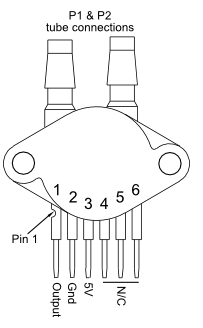
\includegraphics[scale=.65]{./Figures/DisposicionDePinesSensor.png}
\caption{Disposición de pines del sensor de presión MPX5010DP.}
\label{fig:disposición de pines del sensor}
\end{figure}

\section{Planificación}
\label{sec:planificacion}
La planificación original presentada al iniciar el proyecto contemplaba un trabajo de 600 horas. Los atrasos relacionados con la problemática identificada y expuesta en la sección \ref{sec:estructgeneralsistema}, significó repensar un nuevo prototipo con una válvula de control  mecanizada. Esto implicó recurrir a una empresa dedicada a la mecanización de piezas para adaptar el servomotor y una válvula esférica. Como consecuencia de esto, no se pudo contar en tiempo y forma con la pieza total, por lo que se tuvo que modificar la planificación inicial. 
En la tabla \ref{tab:seccplanificacion} se detalla el desglose de tareas pertinente a la planificación original. 
\begin{table}[h]
	\centering
	\caption[Desglose de tareas]{Desglose de tareas}
	\begin{tabular}{l c c}    
		\toprule
		\textbf{WBS}  & \textbf{Tareas} 	 & \textbf{Tiempo[hs]}\\
		\midrule
		1.   & Documentación y Análisis Preliminar	&  19 \\		
		1.1  & Planificación del proyecto			&  24 \\
		1.2  & Análisis de bibliografía especifica &  20 \\
		1.3  & Definición de casos de pruebas		&  15 \\
		2.   & Investigación, Diseño e Implementación & 127 \\
		2.1  & Inicialización del entorno de trabajo  & 34\\
		2.2  & Investigación y diseño del circuito controlador del motor & 12\\
		2.3 & Investigación y diseño del circuito para el sensor lineal &31\\
		2.4 & Definición de la arquitectura del firmware & 54\\
		2.5 & Definición de las interfaces y API’s  &32\\
		2.6 & Implementación de módulo controlador de motor &15\\
		2.7 & Implementación de módulos de adquisición de datos &12\\
		2.8 & Implementación de módulo de comunicación & 16\\
		2.9 & Implementación de herramientas de testing & 18\\
		2.10 & Integración de módulos & 21\\
		2.11 & Investigación  del sensor de presión diferencial & 15\\
		2.12 & Calibración del sensor de presión diferencial y diseño del circuito &13\\
		3. & Verificación y Validación & 48\\
		3.1 & Pruebas unitarias en submódulos &24\\
		3.2 & Pruebas de integración &19\\
		3.3 & Pruebas de Sistema &23\\
		4. & Cierre & 36\\
		4.1 & Elaboración del Informe del proyecto & 24\\
		4.2 & Elaboración de presentación final del proyecto &12\\
		\bottomrule
		\hline
	\end{tabular}
	\label{tab:seccplanificacion}
\end{table}

%Cuando se quiere poner una lista tabulada, se hace así:
%
%\begin{itemize}
%	\item Este es el primer elemento de la lista.
%	\item Este es el segundo elemento de la lista.
%\end{itemize}
%
%Notar el uso de las mayúsculas y el punto al final de cada elemento.
%
%Si se desea poner una lista numerada el formato es este:
%
%\begin{enumerate}
%	\item Este es el primer elemento de la lista.
%	\item Este es el segundo elemento de la lista.
%\end{enumerate}
%
%Notar el uso de las mayúsculas y el punto al final de cada elemento.
%
%\subsection{Este es el título de una subsección}
%\label{subsec:ejemplo}
%
%Se recomienda no utilizar \textbf{texto en negritas} en ningún párrafo, ni tampoco texto \underline{subrayado}. En cambio sí se debe utilizar \textit{texto en itálicas} para palabras en un idioma extranjero, al menos la primera vez que aparecen en el texto. En el caso de palabras que estamos inventando se deben utilizar ``comillas'', así como también para citas textuales. Por ejemplo, un \textit{digital filter} es una especie de ``selector'' que permite separar ciertos componentes armónicos en particular.
%
%La escritura debe ser impersonal. Por ejemplo, no utilizar ``el diseño del firmware lo hice de acuerdo con tal principio'', sino ``el firmware fue diseñado utilizando tal principio''. 
%
%El trabajo es algo que al momento de escribir la memoria se supone que ya está concluido, entonces todo lo que se refiera a hacer el trabajo se narra en tiempo pasado, porque es algo que ya ocurrió. Por ejemplo, "se diseñó el firmware empleando la técnica de test driven development".
%
%En cambio, la memoria es algo que está vivo cada vez que el lector la lee. Por eso transcurre siempre en tiempo presente, como por ejemplo:
%
%``En el presente capítulo se da una visión global sobre las distintas pruebas realizadas y los resultados obtenidos. Se explica el modo en que fueron llevados a cabo los test unitarios y las pruebas del sistema''.
%
%Se recomienda no utilizar una sección de glosario sino colocar la descripción de las abreviaturas como parte del mismo cuerpo del texto. Por ejemplo, RTOS (\textit{Real Time Operating System}, Sistema Operativo de Tiempo Real) o en caso de considerarlo apropiado mediante notas a pie de página.
%
%Si se desea indicar alguna página web utilizar el siguiente formato de referencias bibliográficas, dónde las referencias se detallan en la sección de bibliografía de la memoria, utilizado el formato establecido por IEEE en \citep{IEEE:citation}. Por ejemplo, ``el presente trabajo se basa en la plataforma EDU-CIAA-NXP \citep{CIAA}, la cual...''.
%
%\subsection{Figuras} 
%
%Al insertar figuras en la memoria se deben considerar determinadas pautas. Para empezar, usar siempre tipografía claramente legible. Luego, tener claro que \textbf{es incorrecto} escribir por ejemplo esto: ``El diseño elegido es un cuadrado, como se ve en la siguiente figura:''
%
%\begin{figure}[h]
%\centering
%
\includegraphics[scale=.50]{./Figures/cuadradoAzul.png}
%\end{figure}
%
%La forma correcta de utilizar una figura es con referencias cruzadas, por ejemplo: ``Se eligió utilizar un cuadrado azul para el logo, como puede observarse en la figura \ref{fig:cuadradoAzul}''.
%
%\begin{figure}[ht]
%	\centering
%	
\includegraphics[scale=.45]{./Figures/cuadradoAzul.png}
%	\caption{Ilustración del cuadrado azul que se eligió para el diseño del logo.}
%	\label{fig:cuadradoAzul}
%\end{figure}
%
%El texto de las figuras debe estar siempre en español, excepto que se decida reproducir una figura original tomada de alguna referencia. En ese caso la referencia de la cual se tomó la figura debe ser indicada en el epígrafe de la figura e incluida como una nota al pie, como se ilustra en la figura \ref{fig:palabraIngles}.
%
%\begin{figure}[htpb]
%	\centering
%	
\includegraphics[scale=.3]{./Figures/word.jpeg}
%	\caption{Imagen tomada de la página oficial del procesador\protect\footnotemark.}
%	\label{fig:palabraIngles}
%\end{figure}
%
%\footnotetext{Imagen tomada de \url{https://goo.gl/images/i7C70w}}
%
%La figura y el epígrafe deben conformar una unidad cuyo significado principal pueda ser comprendido por el lector sin necesidad de leer el cuerpo central de la memoria. Para eso es necesario que el epígrafe sea todo lo detallado que corresponda y si en la figura se utilizan abreviaturas entonces aclarar su significado en el epígrafe o en la misma figura.
%
%
%
%\begin{figure}[ht]
%	\centering
%	
\includegraphics[scale=.37]{./Figures/questionMark.png}
%	\caption{¿Por qué de pronto aparece esta figura?}
%	\label{fig:questionMark}
%\end{figure}
%
%Nunca colocar una figura en el documento antes de hacer la primera referencia a ella, como se ilustra con la figura \ref{fig:questionMark}, porque sino el lector no comprenderá por qué de pronto aparece la figura en el documento, lo que distraerá su atención.
%
%Otra posibilidad es utilizar el entorno \textit{subfigure} para incluir más de una figura, como se puede ver en la figura \ref{fig:three graphs}. Notar que se pueden referenciar también las figuras internas individualmente de esta manera: \ref{fig:1de3}, \ref{fig:2de3} y \ref{fig:3de3}.
% 
%\begin{figure}[!htpb]
%     \centering
%     \begin{subfigure}[b]{0.3\textwidth}
%         \centering
%         
\includegraphics[width=.65\textwidth]{./Figures/questionMark}
%         \caption{Un caption.}
%         \label{fig:1de3}
%     \end{subfigure}
%     \hfill
%     \begin{subfigure}[b]{0.3\textwidth}
%         \centering
%         
\includegraphics[width=.65\textwidth]{./Figures/questionMark}
%         \caption{Otro.}
%         \label{fig:2de3}
%     \end{subfigure}
%     \hfill
%     \begin{subfigure}[b]{0.3\textwidth}
%         \centering
%         
\includegraphics[width=.65\textwidth]{./Figures/questionMark}
%         \caption{Y otro más.}
%         \label{fig:3de3}
%     \end{subfigure}
%        \caption{Tres gráficos simples}
%        \label{fig:three graphs}
%\end{figure}
%
%El código para generar las imágenes se encuentra disponible para su reutilización en el archivo \file{Chapter2.tex}.
%
%\subsection{Tablas}
%
%Para las tablas utilizar el mismo formato que para las figuras, sólo que el epígrafe se debe colocar arriba de la tabla, como se ilustra en la tabla \ref{tab:peces}. Observar que sólo algunas filas van con líneas visibles y notar el uso de las negritas para los encabezados.  La referencia se logra utilizando el comando \verb|\ref{<label>}| donde label debe estar definida dentro del entorno de la tabla.
%
%\begin{verbatim}
%\begin{table}[h]
%	\centering
%	\caption[caption corto]{caption largo más descriptivo}
%	\begin{tabular}{l c c}    
%		\toprule
%		\textbf{Especie}     & \textbf{Tamaño} & \textbf{Valor}\\
%		\midrule
%		Amphiprion Ocellaris & 10 cm           & \$ 6.000 \\		
%		Hepatus Blue Tang    & 15 cm           & \$ 7.000 \\
%		Zebrasoma Xanthurus  & 12 cm           & \$ 6.800 \\
%		\bottomrule
%		\hline
%	\end{tabular}
%	\label{tab:peces}
%\end{table}
%\end{verbatim}
%
%
%\begin{table}[h]
%	\centering
%	\caption[caption corto]{caption largo más descriptivo}
%	\begin{tabular}{l c c}    
%		\toprule
%		\textbf{Especie} 	 & \textbf{Tamaño} 		& \textbf{Valor}  \\
%		\midrule
%		Amphiprion Ocellaris & 10 cm 				& \$ 6.000 \\		
%		Hepatus Blue Tang	 & 15 cm				& \$ 7.000 \\
%		Zebrasoma Xanthurus	 & 12 cm				& \$ 6.800 \\
%		\bottomrule
%		\hline
%	\end{tabular}
%	\label{tab:peces}
%\end{table}
%
%En cada capítulo se debe reiniciar el número de conteo de las figuras y las tablas, por ejemplo, figura 2.1 o tabla 2.1, pero no se debe reiniciar el conteo en cada sección. Por suerte la plantilla se encarga de esto por nosotros.
%
%\subsection{Ecuaciones}
%\label{sec:Ecuaciones}
%
%Al insertar ecuaciones en la memoria dentro de un entorno \textit{equation}, éstas se numeran en forma automática  y se pueden referir al igual que como se hace con las figuras y tablas, por ejemplo ver la ecuación \ref{eq:metric}.
%
%\begin{equation}
%	\label{eq:metric}
%	ds^2 = c^2 dt^2 \left( \frac{d\sigma^2}{1-k\sigma^2} + \sigma^2\left[ d\theta^2 + \sin^2\theta d\phi^2 \right] \right)
%\end{equation}
%                                                        
%Es importante tener presente que si bien las ecuaciones pueden ser referidas por su número, también es correcto utilizar los dos puntos, como por ejemplo ``la expresión matemática que describe este comportamiento es la siguiente:''
%
%\begin{equation}
%	\label{eq:schrodinger}
%	\frac{\hbar^2}{2m}\nabla^2\Psi + V(\mathbf{r})\Psi = -i\hbar \frac{\partial\Psi}{\partial t}
%\end{equation}
%
%Para generar la ecuación \ref{eq:metric} se utilizó el siguiente código:
%
%\begin{verbatim}
%\begin{equation}
%	\label{eq:metric}
%	ds^2 = c^2 dt^2 \left( \frac{d\sigma^2}{1-k\sigma^2} + 
%	\sigma^2\left[ d\theta^2 + 
%	\sin^2\theta d\phi^2 \right] \right)
%\end{equation}
%\end{verbatim}
%
%Y para la ecuación \ref{eq:schrodinger}:
%
%\begin{verbatim}
%\begin{equation}
%	\label{eq:schrodinger}
%	\frac{\hbar^2}{2m}\nabla^2\Psi + V(\mathbf{r})\Psi = 
%	-i\hbar \frac{\partial\Psi}{\partial t}
%\end{equation}
%
%\end{verbatim} 
%	\chapter{Diseño e implementación} % Main chapter title
En este capítulo se exponen las tomas decisiones relacionadas al diseño e implementación relacionada al hardware y firmware a lo largo del desarrollo del trabajo. 
\label{Chapter3} % Change X to a consecutive number; for referencing this chapter elsewhere, use \ref{ChapterX}

\definecolor{mygreen}{rgb}{0,0.6,0}
\definecolor{mygray}{rgb}{0.5,0.5,0.5}
\definecolor{mymauve}{rgb}{0.58,0,0.82}

%%%%%%%%%%%%%%%%%%%%%%%%%%%%%%%%%%%%%%%%%%%%%%%%%%%%%%%%%%%%%%%%%%%%%%%%%%%%%
% parámetros para configurar el formato del código en los entornos lstlisting
%%%%%%%%%%%%%%%%%%%%%%%%%%%%%%%%%%%%%%%%%%%%%%%%%%%%%%%%%%%%%%%%%%%%%%%%%%%%%
\lstset{ %
  backgroundcolor=\color{white},   % choose the background color; you must add \usepackage{color} or \usepackage{xcolor}
  basicstyle=\footnotesize,        % the size of the fonts that are used for the code
  breakatwhitespace=false,         % sets if automatic breaks should only happen at whitespace
  breaklines=true,                 % sets automatic line breaking
  captionpos=b,                    % sets the caption-position to bottom
  commentstyle=\color{mygreen},    % comment style
  deletekeywords={...},            % if you want to delete keywords from the given language
  %escapeinside={\%*}{*)},          % if you want to add LaTeX within your code
  %extendedchars=true,              % lets you use non-ASCII characters; for 8-bits encodings only, does not work with UTF-8
  %frame=single,	                % adds a frame around the code
  keepspaces=true,                 % keeps spaces in text, useful for keeping indentation of code (possibly needs columns=flexible)
  keywordstyle=\color{blue},       % keyword style
  language=[ANSI]C,                % the language of the code
  %otherkeywords={*,...},           % if you want to add more keywords to the set
  numbers=left,                    % where to put the line-numbers; possible values are (none, left, right)
  numbersep=5pt,                   % how far the line-numbers are from the code
  numberstyle=\tiny\color{mygray}, % the style that is used for the line-numbers
  rulecolor=\color{black},         % if not set, the frame-color may be changed on line-breaks within not-black text (e.g. comments (green here))
  showspaces=false,                % show spaces everywhere adding particular underscores; it overrides 'showstringspaces'
  showstringspaces=false,          % underline spaces within strings only
  showtabs=false,                  % show tabs within strings adding particular underscores
  stepnumber=1,                    % the step between two line-numbers. If it's 1, each line will be numbered
  stringstyle=\color{mymauve},     % string literal style
  tabsize=2,	                   % sets default tabsize to 2 spaces
  title=\lstname,                  % show the filename of files included with \lstinputlisting; also try caption instead of title
  morecomment=[s]{/*}{*/}
}


%----------------------------------------------------------------------------------------
%	SECTION 1
%----------------------------------------------------------------------------------------
\section{Hardware}
\subsection{Construcción de la válvula de control}
\label{subsec:Construcción de la válvula de control}
Para la fabricación del prototipo fue preciso mecanizar una pieza la cual es una caja desmultiplicadora de fuerza que controla una válvula mediante la energización de un servomotor paso a paso. 
Al emplear una válvula de control fue importante estudiar sus características de funcionamiento. 
La válvula es un mecanismo que permite regular el flujo  o caudal, en este caso de agua, entre dos partes del sistema. 
Básicamente la válvula es un ensamblaje compuesto de un cuerpo con conexión a una tubería y de un obturador operado por accionamiento, donde su función principal es variar el caudal del fluido que circula a través de ella, comportándose como un orificio cuya área está continuamente variando. Las válvulas son uno de los instrumentos de control esenciales en la industria.
Debido a su diseño y materiales, las válvulas pueden abrir y cerrar, conectar y desconectar, regular, modular o aislar un enorme  flujo de líquidos y gases.
El obturador determina la característica de caudal de la válvula; es decir, la relación que existe entre la posición del obturador y el caudal de paso del fluido.
El obturador de una válvula, conforme se va desplazando, produce un área de pasaje que posee una determinada relación característica entre la fracción de carrera de la válvula y el correspondiente caudal que escurre a través de la misma. A esa relación se le da el nombre de característica “inherente” de caudal de válvula.
En este trabajo se utilizó una válvula cuya característica inherente es “Tipo de Apertura Rápida”.
Se trata de una característica que produce una variación grande de caudal a través de la válvula con una carrera pequeña. Este tipo de válvula posibilita el pasaje de casi la totalidad del caudal nominal con apenas una abertura de 25 porciento de la carrera total.
Produce una ganancia muy alta a bajas aperturas de carrera y una ganancia muy baja en aperturas por encima de 60 porciento de carrera total. 
La siguiente figura muestra la curva típica de una válvula de apertura rápida.
\begin{figure}[h]
\centering
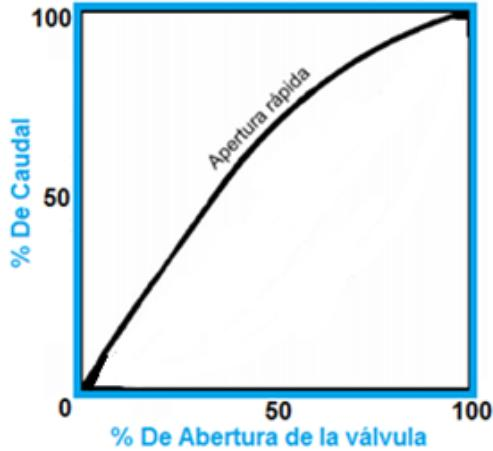
\includegraphics[scale=.50]{./Figures/funcion-valvula.jpeg}
\caption{Gráfica del caudal en función de la apertura de la válvula.}
\label{fig:grafica caudal vs. caudal}
\end{figure}

\subsection{Servomotor}
\label{subsec:Servomotor}
Para el control de la válvula fue necesario un motor que pueda producir un momento de 1 Nm o más. Para este proyecto, por cuestión de disponibilidad, se utilizó un motor paso a paso y un controlador cuyo modelos son 86HS85 y MA860H respectivamente.
El motor paso a paso de 8 hilos posee un torque nominal de 8,5 Nm, suficiente como para realizar movimientos de apertura parcial o total y cierre total de la carrera de dicha válvula, según las necesidades requeridas de caudal. 
El driver MA860H es un controlador para motores paso a paso compatibles con motores 86HS85 con las siguientes características principales:

\begin{enumerate}
	\item Permite ajustar la corriente que se dirige hacia el motor.
	\item Posibilita controlar al motor hasta en 200 micropasos.
	\item Frecuencia de entrada de tren de pulso hasta 300khz. 
	\item Corriente de salida hasta 7.2A.
	\item Entrada TTL compatible y ópticamente aislada.
	\item Soporta modos PUL / DIR y CW / CCW.
\end{enumerate}
El MA860H tiene dos conectores, el conector P1 para conexiones de señales de control y el conector P2 para conexiones de potencia y motor. 
\subsubsection{Configuraciones del conector P1}
PUL+,PUL-: Señal de pulso: esta entrada representa la señal de pulso, activa en cada flanco ascendente o descendente (para este trabajo se encuentra activo en flanco ascendente); 4-5V equivale a un pulso alto y 0-0.5V a un pulso bajo. Para una respuesta confiable, el ancho de pulso debe ser superior a 1,5 microssegundos. 
DIR+;DIR- : Señal DIR: esta señal tiene niveles de voltaje bajo / alto, que representan dos direcciones de rotación del motor. Para una respuesta de movimiento confiable, la señal DIR debe estar por delante de la señal PUL por lo menos 5 microsegundos. 4-5V cuando DIR-HIGH, 0-0.5V cuando DIR-LOW. 

ENA+;ENA-: Señal de Habilitación: esta señal se utiliza para habilitar/deshabilitar el controlador. Nivel alto (la señal de control NPN, PNP y las señales de control diferencial son por el contrario, es decir, nivel bajo para habilitar) para habilitar al controlador y nivel bajo para inhabilitar al controlador.
\subsubsection{Circuito interfaz del conector de señal de control (P1)}
El controlador MA860H puede aceptar entradas diferenciales y de un solo extremo (incluida la salida de colector abierto y PNP). El MA860H tiene 3 entradas lógicas aisladas ópticamente que están ubicadas en el conector P1 para aceptar señales de control del microcontrolador. Estas entradas están aisladas para minimizar o eliminar los ruidos eléctricos acoplados a las señales de control del variador. En la siguiente "Figura \ref{fig:circuito interfaz}", se ilustra las conexiones a colector abierto.
\begin{figure}[h]
\centering
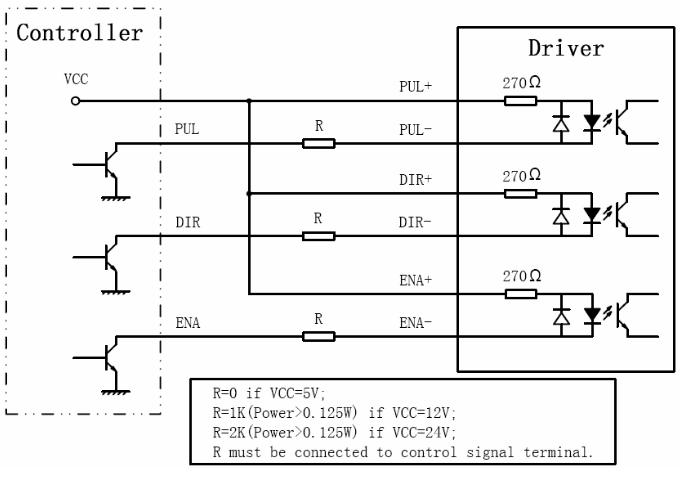
\includegraphics[scale=.65]{./Figures/circuitointerfaz-driver.jpeg}
\caption{Circuito Interfaz - conexiones de señales a colector abierto.}
\label{fig:circuito interfaz}
\end{figure}
Siguiendo las recomendaciones del fabricante relacionadas a la construcción del circuito interfaz entre el diver y el microcontrolador se diseñó y fabricó el circuito eléctrico que se muestra en la "Figura \ref{fig:esquemático circuito interfaz}".

\begin{figure}
\centering
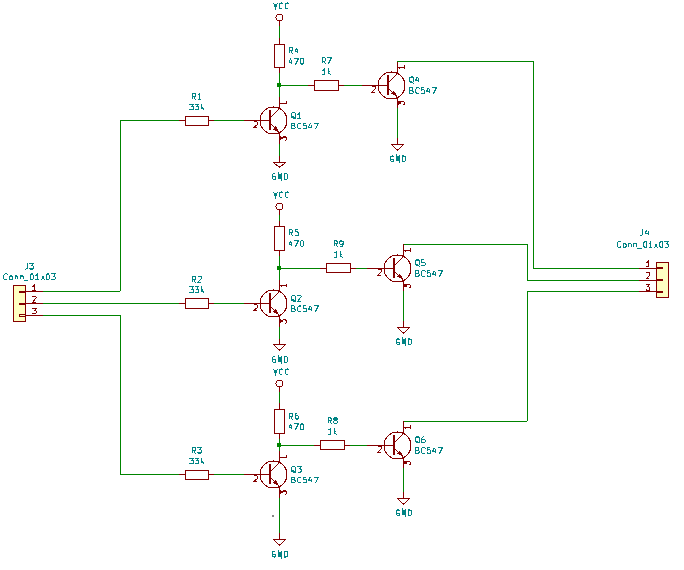
\includegraphics[scale=.85]{./Figures/esquematico-circuito-interfaz.png}
\caption{Esquemático de Circuito Interfaz entre el microcontrolador y driver.}
\label{fig:esquemático circuito interfaz}
\end{figure}

En el esquemático se puede observar dos etapas, la primera es un circuito negador y la segunda corresponde al circuito de colector abierto NPN.
Por todo lo descrito se puede decir que la etapa de potencia está formada por el circuito interfaz y el controlador del motor paso a paso. 
Es importante mencionar que además del motor paso a paso, la electroválvula está constituida por un sensor resistivo de ángulo, que se encuentra adosado al eje de la válvula. La señal derivada de dicho sensor también es retroalimentada y ofrece una estimación de la posición del obturador de la misma. El sensor resistivo es un potenciómetro de una vuelta de 50K ohm cuyo modelo es 91A-503, Bourns cermet.
En la "Figura \ref{fig:Diagrama en bloque de la celda primaria}", podemos observar un diagrama en bloque general que indica entre otras partes del trabajo, cómo está constituido el servomotor.  

\begin{figure}
\centering
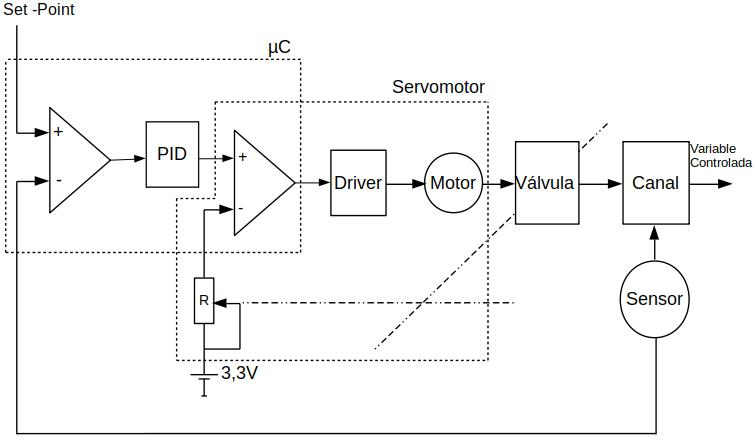
\includegraphics[scale=.65]{./Figures/Diagrama-en-bloque-general-con-servomotor-V2.jpg}
\caption{Diagrama en bloque de la celda primaria.}
\label{fig:Diagrama en bloque de la celda primaria}
\end{figure}
\subsection{Medidor de caudal}
\label{subsec:Medidor de caudal}
La medición del agua es la cuantificación del caudal de agua que pasa por la sección transversal de un río, canal o tubería. También se le conoce como aforo. 
En la mayoría de los casos, la medición del agua resulta de la necesidad de brindar mayor control sobre su uso y distribución. Dicha medición se realiza a través de medidores de caudal. Estos son dispositivos que utilizan diferentes principios mecánicos o físicos para permitir que un flujo de agua pueda ser cuantificado. 
El medidor, que determina la cantidad de fluido que pasa por unidad de tiempo por una sección dada, utilizado en este trabajo para la verificación de caudal de agua proporcionado y además para generar la señal de realimentación correspondiente, es un “Medidor de caudal de Canal Abierto Tipo Aforo”.
Existen varias formas de aforo en canales abiertos, dentro de las principales se encuentran:
\begin{enumerate}
	\item Método volumétrico.
	\item Vertederos.
	\item Canal Parshall. 
	\item Método hidráulico.
\end{enumerate}
Para efectuar el presente trabajo se utilizó el tipo de aforo con vertedero triangular con escotadura en V.
La medición del caudal de las corrientes naturales nunca puede ser exacta debido a que el canal suele ser irregular y por lo tanto es irregular la relación entre nivel y caudal. Los canales de corrientes naturales están también sometidos a cambios debidos a erosión o depósitos. Se pueden obtener cálculos más confiables cuando el caudal pasa a través de una sección donde esos problemas se han limitado. Los vertederos pueden ser definidos como simples aberturas, sobre las cuales un líquido fluye. El término se aplica también a obstáculos en el paso de la corriente y a las excedencias de los embalses. Los vertederos son orificios sin el borde superior y ofrecen las siguientes ventajas en la medición del agua: 

\begin{itemize}
\item Se logra con ellos precisión en los aforos 	
\item La construcción de la estructura es sencilla
\item No son obstruidos por materiales que flotan en el agua 
\item La duración del dispositivo es relativamente larga
\end{itemize}
Los vertederos son utilizados, intensiva y satisfactoriamente en la medición del caudal de pequeños cursos de agua y conductos libres, así como en el control del flujo en galerías y canales.
Para la construcción del vertedero triangular empleado, se precisó de una chapa de hierro plana de 1 mm de espesor, a la que se le  realizó una hendidura de sección triangular, cuyo  valor de ángulo es de 18 grados.
Esta chapa supera los límites del ancho del canal de forma que, ubicándola  verticalmente y en forma transversal al canal, opera como un embalse que por su hendidura sale un flujo de agua.
De esta forma se puede medir en distintos lugares del recorrido del canal, cuál es el caudal real que está pasando por ese punto en particular.  
La "Figura \ref{fig:Placa de aforo}",  muestra la vista de frente de una estructura de un vertedero con escotadura en V. 	
\begin{figure}
\centering
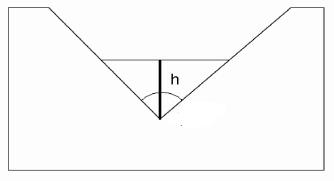
\includegraphics[scale=.85]{./Figures/PlacaDeAforo.jpeg}
\caption{Placa de aforo: vista de frente.}
\label{fig:Placa de aforo}
\end{figure}
La "Figura \ref{fig:Placa de aforo-VistaLateral}", ilustra la vista lateral del vertedero y cómo fluye el líquido por su abertura.
\begin{figure}
\centering
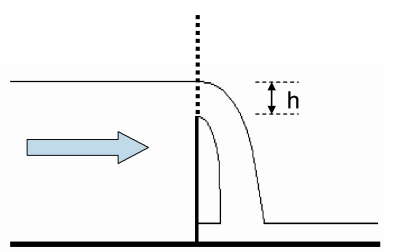
\includegraphics[scale=.85]{./Figures/PlacaDeAforo-VistaLateral.png}
\caption{Placa de aforo: vista lateral.}
\label{fig:Placa de aforo-VistaLateral}
\end{figure}
Entonces, para el calcular el caudal se debe tener en cuenta la siguiente fórmula:
\begin{equation}
 \label{eq:caudal}
 Q = \frac{8}{15}\sqrt{2g} c \tan\alpha  H^\frac{2}{5} 
\end{equation}
	
\begin{figure}
\centering
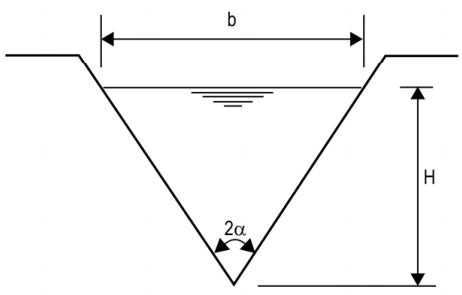
\includegraphics[scale=.75]{./Figures/DimensionesPlacaAforo.png}
\caption{Placa de aforo: dimensiones.}
\label{fig:Placa de aforo dimensiones}
\end{figure}	

Teniendo en cuenta la ecuación \ref{eq:caudal}
\begin{itemize}
\item Q: es caudal en m3/seg
\item g: coeficiente de gravedad
\item c: coeficiente de descarga
\item alpha: ángulo del vertedero
\item H: nivel de agua en metros

\end{itemize}

Los medidores de caudal con aforo triangular como el utilizado en el presente trabajo, responden a una ecuación del modelo que se expone arriba y la misma se obtuvo empíricamente. En el caso de este proyecto y por tratarse de un prototipo a escala, es un medidor que se usará por única vez, por lo tanto la tabla de calibración del caudalímetro fue obtenida experimentalmente.  
En la "Figura \ref{fig:alturas vertedero}", se detalla la vista de frente del canal con el vertedero triangular y los diversos niveles de altura que se consideraron al momento de realizar las mediciones pertinentes. 

\begin{figure}
\centering
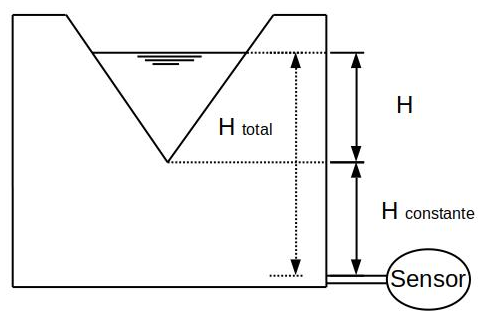
\includegraphics[scale=.75]{./Figures/AlturaVertedero.png}
\caption{Placa de aforo: dimensiones.}
\label{fig:alturas vertedero}
\end{figure}
A partir de la "Figura \ref{fig:alturas vertedero}", se intenta especificar que existe una manguera, la cual uno de sus extremos se conecta a la base del canal y el otro a una de las dos espigas del sensor. Además, se puede advertir los niveles de altura que se deben tener en cuenta. H total corresponde a la altura entre el nivel de agua en un instante dado y la manguera conectada al sensor, H constante se encuentra asociada al nivel de altura que está comprendido entre dicha manguera y el vértice del triángulo del vertedero, y finalmente H variable es la altura que está contenida entre el nivel de agua y el vértice del triángulo de dicho vertedero.    
Por lo tanto, este caudalímetro de canal abierto por sistema de aforo utiliza como medidor de nivel de columna de agua un sensor de presión cuyo modelo es MPX5010DP. 
Este transductor piezo-resistivo, es un sensor de presión de silicio monolítico que puede ser utilizado en aplicaciones que disponen de un microcontrolador o microprocesador con entradas ADC.
El MPX5010DP entrega a su salida un rango de voltaje entre 0v y 5v, mediante esta información y una fórmula que se expone en el siguiente párrafo se puede estimar la presión hasta un valor de 10 KPa, esto es, una columna de agua de hasta 100 cm de altura.
Esta señal proveniente del sensor en conjunto con un algoritmo de control PID, permite regular el caudal de agua en un determinado valor preestablecido. 
El dispositivo proporciona una salida lineal como puede se observar en la "Figura \ref{fig:función de salida del sensor}", extraída de su hoja de datos.

\begin{figure}
\centering
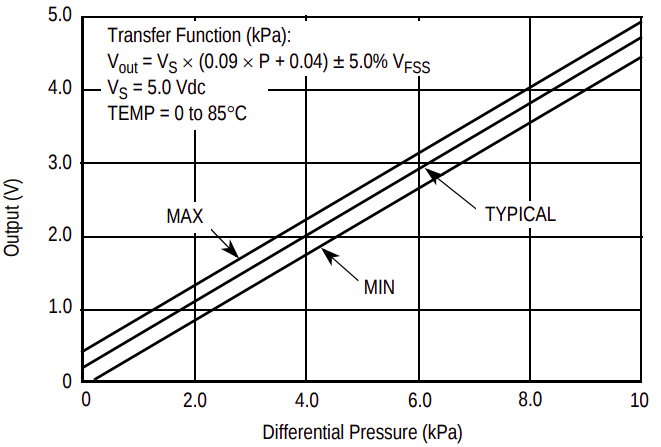
\includegraphics[scale=.55]{./Figures/SalidaMPX5010DP.png}
\caption{Función de salida del sensor de presión MPX5010DP.}
\label{fig:función de salida del sensor}
\end{figure}
Como se pudo observar el gráfico anterior de la "Figura \ref{fig:función de salida del sensor}", la ecuación para obtener la presión del sensor viene dada por la ecuación \ref{eq:presion}:
\begin{equation}
 \label{eq:presion}
 P = \frac{Vout- 0.04*Vs \pm Tol}{0.09*Vs}
\end{equation}
Vs es el valor de voltaje de alimentación Vs = 5v, Vout es el valor de voltaje que entrega el sensor, Tol es la tolerancia, un ajuste que se debe aplicar al sensor para  calibrar a medida.
Tomando como base la ecuación de presión diferencial que relaciona la altura se resuelve que (recordando que la presión a la atmósfera es cero):  

\begin{equation}
 \label{eq:presión}
	 P =PH -PL= P = gh =\frac{Vout- 0.04*Vs \pm Tol}{0.09*Vs}	
\end{equation}
 Donde P es la presión,  es la densidad del agua, g es la gravedad y h es el nivel de la columna líquida.

La disposición de los pines del dispositivo lo podemos advertir en la "Figura \ref{fig:disposición de pines del sensor}":
\begin{figure}
\centering
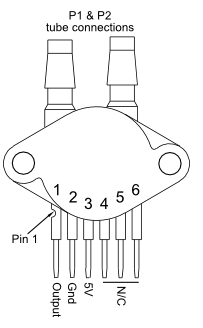
\includegraphics[scale=.65]{./Figures/DisposicionDePinesSensor.png}
\caption{Disposición de pines del sensor de presión MPX5010DP.}
\label{fig:disposición de pines del sensor}
\end{figure}

Siendo la densidad del agua =1000 kgm3  y la gravedad g=10ms2
La ecuación resultante para obtener h es: h=Pg. 
Una vez construido el prototipo, se realizó una calibración de caudal obteniéndose una tabla Caudal vs Htotal (altura). Por lo que, en el firmware esta tabla es utilizada para obtener el valor de caudal  en lugar de la fórmula presentada.
\section{Software}
\subsection{Arquitectura de software}
\label{subsec:Arquitectura de software}

Durante la definición de la arquitectura de software se seleccionaron dos arquitecturas de software y se integraron para confeccionar una arquitectura híbrida, de modo tal que se adapte a las necesidades concretas de este proyecto. Por un lado, se seleccionó una arquitectura en capas, la cual está conformada por tres capas claramente definidas.
En la capa HAL se encuentran los drivers encargados de abstraer los detalles de acceso al hardware. De esta forma, facilitará la migración a otro microcontrolador en caso de que en el futuro hiciese falta. Adicionalmente, permite una mayor claridad en la implementación, separando los drivers de la lógica de la aplicación.
Debido a que en producción se utilizará como hardware a la CIAA-NXP y durante el desarrollo la EDU-CIAA-NXP, se empleó el firmware de la CIAA versión 3.0 como capa de abstracción de hardware. 
En la capa de aplicación se encuentran todos los componentes que encapsulan la lógica de aplicación, y finalmente, la tercera corresponde al sistema operativo de tiempo real. En esta capa se empleó el sistema operativo FreeRTOS.
El sistema incluye sensores que proveen información relacionada al ámbito a controlar y un actuador que cambian dicho ámbito. Por lo tanto, en respuesta a las alteraciones identificadas por los sensores, se envían señales de control a los actuadores del sistema. Entonces, al identificar que dicho sistema debe poseer este tipo de comportamiento se definió emplear una arquitectura de tiempo real inherente al “Control Ambiental”, ya que este patrón de arquitectura de software brinda la posibilidad de recopilar datos del entorno por medio de sensores como así también el estado en el que se encuentran los actuadores  conectados al sistema. Con base en datos reunidos de sensores y actuador, se envían señales de control hacia el actuador para producir cambios en dicho entorno controlado. En la "Figura \ref{fig:Arquitectura de software}", se puede ver el diagrama del patrón arquitectónico que es la base del diseño del sistema de control, y además utilizado en la capa aplicación. 

\begin{figure}
\centering
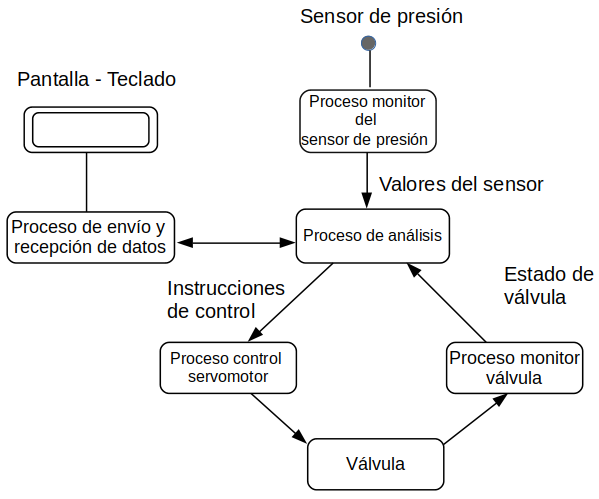
\includegraphics[scale=.65]{./Figures/ArquitecturaSoftware.png}
\caption{Arquitectura de sistema de control de caudal de agua en canal a cielo abierto.}
\label{fig:Arquitectura de software}
\end{figure}

Al aplicar ambos patrones se constituyó un patrón híbrido de dos capas. La capa inferior es la capa de abstracción de hardware. La capa superior, pertenece a la aplicación.

\subsection{Componentes de software}
\label{subsec:Componentes de software}
Cada capa de software es considerada un componente de software. Con lo cual se poseen los siguientes componentes:

\begin{itemize}
\item HAL
\item Sistema Operativo
\item Aplicación
\end{itemize}

A su vez, la capa de aplicación está compuesta por los siguientes componentes de software:

\begin{itemize}
\item Monitor sensor de presión.
\item Control servomotor.
\item Monitor válvula.
\item Control de recepción y envío de datos.
\end{itemize}

En la "Figura \ref{fig:Capas de componentes de software}", se puede apreciar el nivel de jerarquía de cada una de las capas siendo la capa HAL la  más baja: 

\begin{figure}
\centering
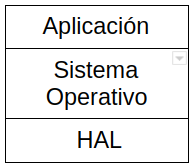
\includegraphics[scale=.75]{./Figures/JerarquiaDeCapas-Software.png}
\caption{Jerarquía de componentes de software.}
\label{fig:Capas de componentes de software}
\end{figure}
\subsubsection{Diseño detallado}
A continuación se incluye el diseño detallado de cada uno de los componentes de software presentados en la "Figura \ref{fig:Arquitectura de software}".
	\begin{figure}
	\centering
	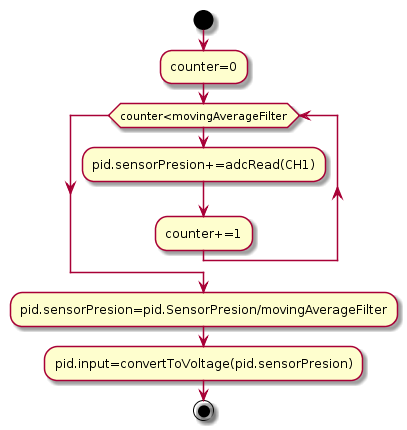
\includegraphics[scale=.65]{./Figures/Procesomonitorsensordepresion.png}
	\caption{Proceso monitor del sensor de presión.}
	\label{fig:Control servomotor}
	\end{figure}
	
\begin{figure}
	\centering
	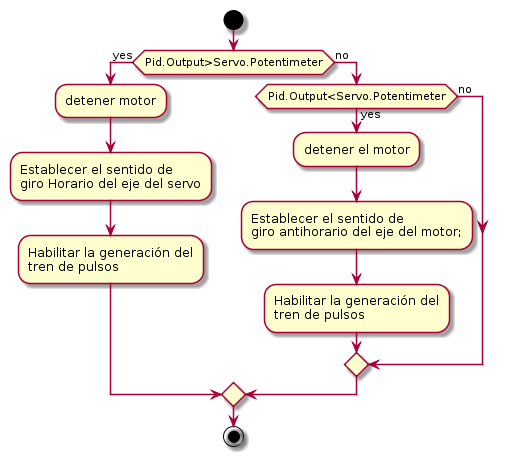
\includegraphics[scale=.55]{./Figures/ProcesoControlServo.png}
	\caption{Proceso de control del servomotor.}
	\label{fig:Control servomotor}
	\end{figure}

 	\begin{figure}
	\centering
	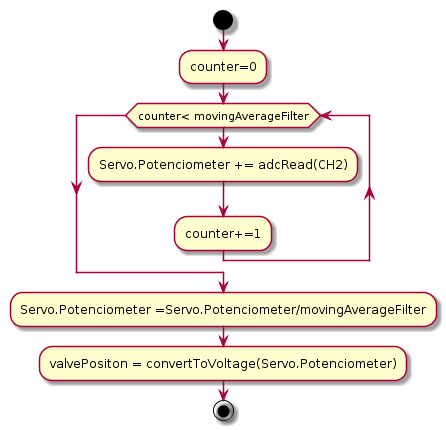
\includegraphics[scale=.65]{./Figures/MonitorValvula.png}
	\caption{Proceso monitor válvula.}
	\label{fig:Proceso monitor valvula}
	\end{figure}

	\begin{figure}
	\centering
	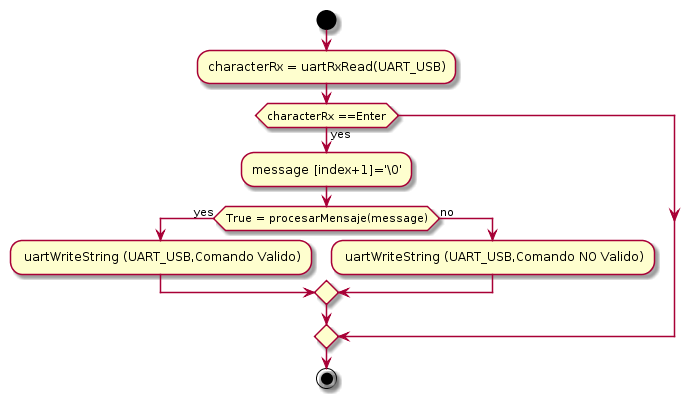
\includegraphics[scale=.65]{./Figures/Porcesorecepcionyenviodedatos.png}
	\caption{Proceso de envió y recepción de datos.}
	\label{fig:Proceso De envió y recepción de datos}
	\end{figure}

	
\begin{figure}
	\centering
	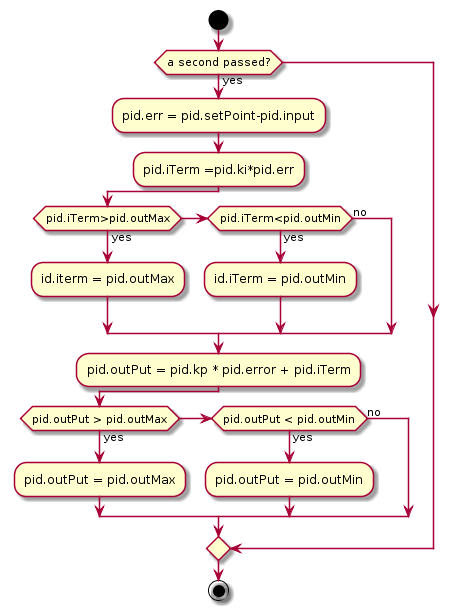
\includegraphics[scale=.65]{./Figures/procesocontrolPID.png}
	\caption{Proceso de Control PID.}
	\label{fig:Proceso de Control PID}
	\end{figure}
\subsection{Casos de uso}
\label{subsec:Casos de uso}
Para la etapa de captura de requerimientos funcionales que el sistema debía satisfacer se emplearon casos de uso correspondientes al Lenguaje Unificado Modelado (UML) ya que es de mucha utilidad y permite especificar, visualizar, construir y documentar los requisitos del sistema especialmente en sistemas con un alto grado de interacción hombre/máquina. A continuación se presentan dos casos de uso considerados como principales.

\subsubsection{Caso de uso: detectar el nivel de agua del canal}
\begin{table}[t]
\begin{center}
\begin{tabular}{ | m{4cm} | m{9.5cm} | }
\hline Nombre & Detectar el nivel de agua del canal \\ \hline
1.1 Breve descripción & 
El firmware debe detectar por medio del sensor de presión el nivel de agua existente en el canal. \\ \hline

 1.2 Actor Principal&La aplicación móvil.\\ \hline


 1.3 Disparadores & La recepción de un comando. \\ \hline

Flujo de Eventos& \\ \hline

 2.1 Flujo básico &
El firmware recibe el paquete desde un smartphone  o desde una aplicación de comunicación serial desde una pc. \\ \hline


 2.1.2 Flujo básico &
El firmware deberá desencapsular el comando recibido y extraer los diferentes campos de información. \\ \hline

 2.1.3 Flujo básico &
El firmware deberá identificar el tipo de operación. \\ \hline


 2.1.4 Flujo básico &
El firmware deberá leer un pin configurado como adc asociado al sensor de presión un valor digital. \\ \hline
 

2.1.5 Flujo básico &
Se repite el paso 2.1.4 hasta 5 veces, de forma que el firmware deberá realizar una acumulación de los valores obtenidos. \\ \hline


2.1.6 Flujo básico &
 El firmware con base al acumulador obtenido en el punto anterior deberá, realizar un filtro de promedio móvil.  \\ \hline
 
2.1.7 Flujo básico &
El firmware deberá convertir el valor digital promediado a tensión. \\ \hline 
2.1.8 Flujo básico &
El firmware deberá obtener el nivel de agua con el dato obtenido en el punto anterior empleando una tabla que se obtendrá experimentalmente. \\ \hline
2.1.9 Flujo básico &
El firmware deberá controlar si el resultado se encuentra dentro de las dimensiones establecidas. \\ \hline
2.1.10 Flujo básico &
El firmware deberá enviar por el puerto serial el valor de nivel de agua en cm. \\ \hline
2.2 Flujo alternativo &  \\ \hline


2.2.1 Flujo alternativo  & 
2.1.9 Si la distancia obtenida se encuentra fuera de rango se enviará por la UART “Distancia Fuera de Rango - Verificar el correcto Funcionamiento del  sensor”. \\ \hline

Requisitos Especiales & \\ \hline


Pre - condiciones & \\ \hline
 
4.1 Pre - condiciones & 
El firmware debe estar en estado de correcto funcionamiento. \\ \hline

4.2 Pre - condiciones &
La comunicación serial se debe encontrar en condiciones óptimas para su funcionamiento correcto. \\ \hline

Post- Condiciones &
El firmware deberá quedar operativo y en correcto 
funcionamiento y en condiciones para la recepción de futuros comandos. \\ \hline

\end{tabular}
\caption{ Caso de uso: detectar el nivel de agua del canal.}
\label{tab:coches}
\end{center}
\end{table}

\subsubsection{Caso de uso:establecer un determinado valor de caudal.}

\begin{table}[t]
\begin{center}
\begin{tabular}{ | m{4cm} | m{9cm} | }
\hline 
Nombre & Establecer un determinado de valor de caudal.\\ \hline
1.1 Breve descripción &
El firmware debe establecer un caudal mediante la manipulación de la posición de la válvula de control.\\ \hline
 1.2 Actor Principal & La aplicación móvil.\\ \hline
 1.3 Disparadores & La recepción de un comando \\ \hline
Flujo de Eventos & \\ \hline


 2.1 Flujo básico &
El firmware recibe el paquete desde un smartphone  o desde una aplicación de comunicación serial desde una pc. \\ \hline
 2.1.2 Flujo básico &
El firmware deberá desencapsular el comando recibido y extraer los diferentes campos de información. \\ \hline
 2.1.3 Flujo básico &
El firmware deberá identificar el tipo de operación. \\ \hline


 2.1.4 Flujo básico &
El firmware deberá leer un pin configurado como adc asociado al sensor de presión un valor digital. \\ \hline


2.1.5 Flujo básico &
Se repite el paso 2.1.4 hasta 5 veces, de forma que el firmware deberá realizar una acumulación de los valores obtenidos.\\ \hline
2.1.6 Flujo básico &
 El firmware con base al acumulador obtenido en el punto anterior deberá, realizar un filtro de promedio móvil.  \\ \hline
2.1.7 Flujo básico & 
El firmware deberá convertir el valor digital promediado a tensión.  \\ \hline
2.1.8 Flujo básico & 
El firmware deberá obtener el caudal con el dato obtenido en el punto anterior empleando una tabla que se obtendrá experimentalmente. \\ \hline
2.1.9 Flujo básico &
El firmware deberá comparar este resultado de caudal obtenido con el set point. \\ \hline
2.1.10 Flujo básico &
En caso de ser valores diferentes, el firmware deberá generar un tren de pulsos hasta posicionar la válvula de control. \\ \hline
2.1.11 Flujo básico &
Se repite desde 2.1.4 hasta que el caudal obtenido a través del sensor y el set point sean iguales. \\ \hline
2.2 Flujo alternativo & \\ \hline


2.2.1 Flujo alternativo & 
2.1.10 Si los valores son iguales el firmware deberá detener la generación del tren de pulsos. \\ \hline
Requisitos Especiales & \\ \hline


Pre - condiciones & \\ \hline
 
4.1 Pre - condiciones &
El firmware debe estar en estado de correcto funcionamiento. \\ \hline
4.2 Pre - condiciones &
La comunicación serial se debe encontrar en condiciones óptimas para su funcionamiento correcto. \\ \hline
Post- Condiciones &
El firmware deberá quedar operativo y en correcto funcionamiento y en condiciones para la recepción de futuros comandos.\\ \hline
\end{tabular}
\caption{ Caso de uso: establecer un determinado valor de caudal.}
\label{tab:establecer un determinado valor de caudal.}
\end{center}
\end{table}

\subsection{Diagrama de clase}
\label{subsec:Diagrama de clase}
Al momento de desarrollar el firmware, de forma previa se realizó un diagrama de clase, que se puede ver en la "Figura \ref{fig:Diagrama de clase.}". 
\begin{figure}
	\centering
	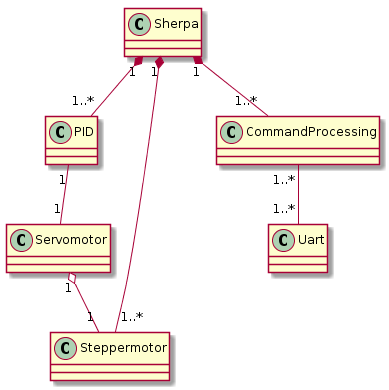
\includegraphics[scale=.75]{./Figures/DiagramaDeClase-DistribucionDeAgua.png}
	\caption{Diagrama de clase.}
	\label{fig:Diagrama de clase.}
	\end{figure}

Uart:  
este módulo recibe y envía los comandos desde y hacia la aplicación de comunicación serial que se ejecuta en la PC.

Command Processing:
acumulará y convertirá de carácter a decimal los comandos recibidos y los devuelve cuando sea solicitado



Stepper Motor:
este módulo posee todas las funciones inherentes al control del motor paso a paso. Interactúa con el módulo Servomotor para integrar las características de un servomotor convencional. 

Servomotor:
el propósito de Servomotor es establecer la posición de la válvula realizando una comparación entre el resultado que se va obteniendo del algoritmo de control PID, output y la posición actual de dicha válvula.

PID:  
este módulo implementa un algoritmo de control PID. El mismo es ejecutado cada un segundo para cuantificar el error o desviación que existe entre el valor de caudal medido a través del sensor de presión y el valor deseado. Este valor es solicitado por el módulo Servomotor.
\subsection{Protocolo de comunicación}
\label{subsec:Protocolo de comunicación}
Se definió un paquete de datos  para que el usuario pueda testear todos los comandos que involucre el servomotor y verificar su correcto funcionamiento. A continuación se detalla lo siguiente:
\begin{enumerate}
\item Habilitar o deshabilitar el motor.
\item Establecer los micro pasos (MicroStep).
\item Establecer el sentido de giro(Horario/Antihorario).
\item Cantidad de pasos a realizar.
\item El ángulo a girar.
\item Cantidad de vueltas a girar.
\end{enumerate}
Un vez validado el funcionamiento del servomotor se procedió de estructurar los comandos validos del sistema.
\begin{itemize}
\item Habilitar el motor: ME \\
		\hspace{1cm} M: Motor	\\
		\hspace{1cm} E: Habilitar 
\item Deshabilitar el motor: MD \\
		M: Motor \\
		D: Deshabilitar
\item Establecer los micropasos: MMSF, MMSH, MMS04, MMS08, MMS16, MMS32 \\
		M: Motor \\
		MS: MicroSteps \\
		F: Full step \\
		H: Half step \\
		04: 1/4 step \\
		08: 1/8 step \\
		16: 1/16 step \\
		32: 1/32 step 
\item Establecer el sentido de giro del eje del motor: MTH, MTA.\\
		M: Motor. \\
		T: Turn (giro) \\
		H: Horario. \\
		A: Antihorario \\
		
		‘0’ lógico antihorario \\
		’1' lógico	 horario 		
\item	Establecer la cantidad de pasos: MS1201. \\
		M: Motor \\
		S: Step \\
		1201: 4 dígitos para el número de pasos 
\item	Establece el ángulo de giro del eje del motor: MA0360. \\
		M: Motor \\
		A: Ángulo \\
		0360: 4 dígitos para especificar el valor del ángulo 
\item  Establece la cantidad de vueltas que deberá girar el eje del motor: MFT003. \\
    M: Motor \\
    FT: Full Turns(vueltas completadas) \\
    003: 3 dígitos para especificar el valor de las vueltas completas 
\item Establecer el Set Point del control PID: SP075. \\
   SP: Set Point \\
   075: Porcentaje correspondiente al máximo del caudal 
\item Detectar el nivel de agua: NA(nivel de agua).

\end{itemize}

Al final de cada una de las tramas, se incorpora el carácter de salto de línea que indica el límite final del comando. Una vez recibido el mismo, este pasa a ser procesado por una función, de forma que si presenta un error, el firmware envía por el mismo medio una cadena “comando invalido”, caso contrario “comando válido”. 
\subsection{Algoritmo PID}
\label{subsec:Algoritmo PID}
Durante el diseño del proyecto se identificó la posibilidad de implementar un control de proceso con realimentación. La tarea particular del sistema de control, es la de determinar y actualizar la posición de la válvula a medida que cambian las condiciones de carga hasta que la variable controlada, caudal, alcance el valor deseado, y permanecer allí indefinidamente aún produciéndose perturbaciones externas. Con base a las necesidades expuestas se definió incorporar al firmware un algoritmo de control PID como una herramienta tecnológica que permite cuantificar el error o desviación que existe entre un valor medido y un valor deseado de caudal. El mismo está basado en el algoritmo publicado por Brett Beauregard y se modificó para satisfacer las necesidades concretas del presente proyecto. Es útil destacar que se seleccionó un modo de control que consiste en una combinación de la acción integral con la acción proporcional eliminando la acción derivativa.   
Cuando el control es una válvula la acción derivativa no se utiliza. Porque la parte derivativa tiene justamente la propiedad de actuar en un porcentaje muy elevado de la salida ante variaciones muy pequeñas del error, es decir la entrada. Es la parte del algoritmo que se añadió al final de todo, para acelerar la acción de control. Por la naturaleza matemática    del algoritmo, la acción de control de la parte derivativa es muy elevada en porcentaje aunque el error sea pequeño, ante cualquier variación se establece un porcentaje de salida muy grande. Esto hace que ante cualquier pequeña variación del error, la válvula reaccione ante la salida fuertemente abriéndose y cerrándose. Estos movimientos repetitivos, lógicamente terminan rompiendo la válvula. Es por esto que la acción derivativa no se utiliza cuando el actuador del sistema de control es una válvula. 

%A modo de ejemplo:
%
%\begin{lstlisting}[label=cod:vControl,caption=Pseudocódigo del lazo principal de control.]  % Start your code-block
%
%#define MAX_SENSOR_NUMBER 3
%#define MAX_ALARM_NUMBER  6
%#define MAX_ACTUATOR_NUMBER 6
%
%uint32_t sensorValue[MAX_SENSOR_NUMBER];		
%FunctionalState alarmControl[MAX_ALARM_NUMBER];	//ENABLE or DISABLE
%state_t alarmState[MAX_ALARM_NUMBER];						//ON or OFF
%state_t actuatorState[MAX_ACTUATOR_NUMBER];			//ON or OFF
%
%void vControl() {
%
%	initGlobalVariables();
%	
%	period = 500 ms;
%		
%	while(1) {
%
%		ticks = xTaskGetTickCount();
%		
%		updateSensors();
%		
%		updateAlarms();
%		
%		controlActuators();
%		
%		vTaskDelayUntil(&ticks, period);
%	}
%}
%\end{lstlisting}
%
%
%

%	% Chapter Template

\chapter{Ensayos y Resultados} % Main chapter title

\label{Chapter4} % Change X to a consecutive number; for referencing this chapter elsewhere, use \ref{ChapterX}

%----------------------------------------------------------------------------------------
%	SECTION 1
%----------------------------------------------------------------------------------------

\section{Pruebas funcionales del hardware}
\label{sec:pruebasHW}

La idea de esta sección es explicar cómo se hicieron los ensayos, qué resultados se obtuvieron y analizarlos.
 
%	% Chapter Template

\chapter{Conclusiones} % Main chapter title

\label{Chapter5} % Change X to a consecutive number; for referencing this chapter elsewhere, use \ref{ChapterX}


%----------------------------------------------------------------------------------------

%----------------------------------------------------------------------------------------
%	SECTION 1
%----------------------------------------------------------------------------------------

\section{Conclusiones generales }

La idea de esta sección es resaltar cuáles son los principales aportes del trabajo realizado y cómo se podría continuar. Debe ser especialmente breve y concisa. Es buena idea usar un listado para enumerar los logros obtenidos.

Algunas preguntas que pueden servir para completar este capítulo:

\begin{itemize}
\item ¿Cuál es el grado de cumplimiento de los requerimientos?
\item ¿Cuán fielmente se puedo seguir la planificación original (cronograma incluido)?
\item ¿Se manifestó algunos de los riesgos identificados en la planificación? ¿Fue efectivo el plan de mitigación? ¿Se debió aplicar alguna otra acción no contemplada previamente?
\item Si se debieron hacer modificaciones a lo planificado ¿Cuáles fueron las causas y los efectos?
\item ¿Qué técnicas resultaron útiles para el desarrollo del proyecto y cuáles no tanto?
\end{itemize}


%----------------------------------------------------------------------------------------
%	SECTION 2
%----------------------------------------------------------------------------------------
\section{Próximos pasos}

Acá se indica cómo se podría continuar el trabajo más adelante.
 
%\end{verbatim}
%
%Los apéndices también deben escribirse en archivos .tex separados, que se deben ubicar dentro de la carpeta \emph{Appendices}. Los apéndices vienen comentados por defecto con el caracter \code{\%} y para incluirlos simplemente se debe eliminar dicho caracter.
%
%Finalmente, se encuentra el código para incluir la bibliografía en el documento final.  Este código tampoco debe modificarse. La metodología para trabajar las referencias bibliográficas se desarrolla en la sección \ref{sec:biblio}.
%%----------------------------------------------------------------------------------------
%
%\section{Bibliografía}
%\label{sec:biblio}
%
%Las opciones de formato de la bibliografía se controlan a través del paquete de latex \option{biblatex} que se incluye en la memoria en el archivo memoria.tex.  Estas opciones determinan cómo se generan las citas bibliográficas en el cuerpo del documento y cómo se genera la bibliografía al final de la memoria.
%
%En el preámbulo se puede encontrar el código que incluye el paquete biblatex, que no requiere ninguna modificación del usuario de la plantilla, y que contiene las siguientes opciones:
%
%\begin{lstlisting}
%\usepackage[backend=bibtex,
%	natbib=true, 
%	style=numeric, 
%	sorting=none]
%{biblatex}
%\end{lstlisting}
%
%En el archivo \file{reference.bib} se encuentran las referencias bibliográficas que se pueden citar en el documento.  Para incorporar una nueva cita al documento lo primero es agregarla en este archivo con todos los campos necesario.  Todas las entradas bibliográficas comienzan con $@$ y una palabra que define el formato de la entrada.  Para cada formato existen campos obligatorios que deben completarse. No importa el orden en que las entradas estén definidas en el archivo .bib.  Tampoco es importante el orden en que estén definidos los campos de una entrada bibliográfica. A continuación se muestran algunos ejemplos:
%
%\begin{lstlisting}
%@ARTICLE{ARTICLE:1,
%    AUTHOR="John Doe",
%    TITLE="Title",
%    JOURNAL="Journal",
%    YEAR="2017",
%}
%\end{lstlisting}
%
%
%\begin{lstlisting}
%@BOOK{BOOK:1,
%    AUTHOR="John Doe",
%    TITLE="The Book without Title",
%    PUBLISHER="Dummy Publisher",
%    YEAR="2100",
%}
%\end{lstlisting}
%
%
%\begin{lstlisting}
%@INBOOK{BOOK:2,
%    AUTHOR="John Doe",
%    TITLE="The Book without Title",
%    PUBLISHER="Dummy Publisher",
%    YEAR="2100",
%    PAGES="100-200",
%}
%\end{lstlisting}
%
%
%\begin{lstlisting}
%@MISC{WEBSITE:1,
%    HOWPUBLISHED = "\url{http://example.com}",
%    AUTHOR = "Intel",
%    TITLE = "Example Website",
%    MONTH = "12",
%    YEAR = "1988",
%    URLDATE = {2012-11-26}
%}
%\end{lstlisting}
%
%Se debe notar que los nombres \emph{ARTICLE:1}, \emph{BOOK:1}, \emph{BOOK:2} y \emph{WEBSITE:1} son nombres de fantasía que le sirve al autor del documento para identificar la entrada. En este sentido, se podrían reemplazar por cualquier otro nombre.  Tampoco es necesario poner : seguido de un número, en los ejemplos sólo se incluye como un posible estilo para identificar las entradas.
%
%La entradas se citan en el documento con el comando: 
%
%\begin{verbatim}
%\citep{nombre_de_la_entrada}
%\end{verbatim}
%
%Y cuando se usan, se muestran así: \citep{ARTICLE:1}, \citep{BOOK:1}, \citep{BOOK:2}, \citep{WEBSITE:1}.  Notar cómo se conforma la sección Bibliografía al final del documento. 

%	\chapter{Introducción específica} % Main chapter title

\label{Chapter2}

%----------------------------------------------------------------------------------------
%	SECTION 1
%----------------------------------------------------------------------------------------
%Todos los capítulos deben comenzar con un breve párrafo introductorio que indique cuál es el contenido que se encontrará al leerlo.  La redacción sobre el contenido de la memoria debe hacerse en presente y todo lo referido al proyecto en pasado, siempre de modo impersonal.
En este capítulo se abordarán temas referentes al análisis de la estructura del sistema que se desarrolló, gestión, planificación del trabajo y técnicas relacionadas al sensor empleado.  	 

\section{Estructura general del sistema}
\label{sec:estructgeneralsistema}

%\subsection{Uso de mayúscula inicial para los título de secciones}

%Si en el texto se hace alusión a diferentes partes del trabajo referirse a ellas como capítulo, sección o subsección según corresponda. Por ejemplo: ``En el capítulo \ref{Chapter1} se explica tal cosa'', o ``En la sección \ref{sec:ejemplo} se presenta lo que sea'', o ``En la subsección \ref{subsec:ejemplo} se discute otra cosa''.
 
En un plano para la construcción del prototipo a escala, se pudo reconocer un inconveniente. Al emplear una compuerta que se desplaza verticalmente y ubicada en forma perpendicular al canal, se generarían filtraciones de agua en sus guías de desplazamiento. Como se trata de una maqueta a escala, estas filtraciones provocarían errores considerables al momento de realizar las mediciones relacionadas con la altura de la superficie de agua, y cálculos pertinentes al aplicar el método de aforo por compuerta para determinar el caudal. Por lo tanto, en el sistema no se obtendrían los resultados esperados. En este contexto, el caudal que circularía por debajo de la compuerta sería menor que el que se registraría en el caudalímetro. De esta forma, se obtendrían dos valores de caudales diferentes debido, entre otros factores, a las filtraciones.     
Esto motivó a reemplazar, en el prototipo, la compuerta por una válvula y así eliminar los errores que introducen dichas filtraciones. 
Para el control de la válvula se elaboró un servomotor con el empleo de un motor paso a paso con su correspondiente controlador.
En la figura \ref{fig:Vertedero triangular}, se puede apreciar un vertedero triangular en un canal abierto y una regla que mide el nivel de la superficie de agua.
\begin{figure}[h]
\centering
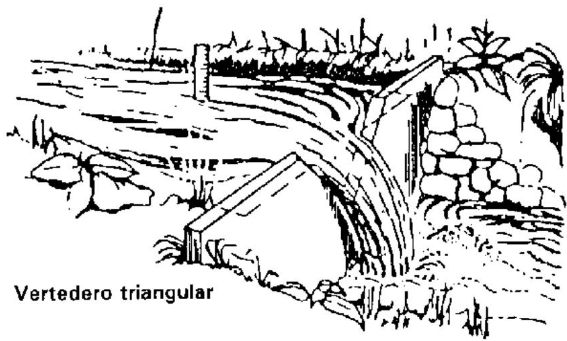
\includegraphics[scale=.60]{./Figures/VertederoTriangular.png}
\caption{Ilustración de un vertedero triangular ubicado en determinado punto a medir caudal en el canal.}
\label{fig:Vertedero triangular}
\end{figure}

Para medir el caudal, se fabricó un caudalímetro por placa de aforo triangular. Estos tipos de instrumentos, también denominados vertederos, representan un dique o pared que intercepta en un determinado punto una corriente de líquido, en este caso agua, con superficie libre, como se puede apreciar en la figura 2.1 . En general, se utilizan para mantener un nivel de superficie de aguas arriba que no exceda de un valor límite, o bien para medir el caudal de agua circulante por un canal. Este instrumento resulta un medidor de caudal sencillo pero efectivo en canales abiertos. 

El principio de funcionamiento de la celda primaria consiste en establecer el caudal de agua a un valor establecido por el usuario. Para llevar a cabo esto, fue necesario el desarrollo de un firmware que controla el eje de un servomotor. Este se encuentra adherido a una válvula, lo que permite maniobrar su rango de apertura para regular el flujo del fluido según las necesidades.

El diagrama de control correspondiente es el que se muestra en la figura \ref{fig:CeldaPrimaria} donde se aprecia que la salida del servomotor actúa directamente sobre la válvula. Esta puede ser una llave esférica, como es este el caso, o un sistema de cremallera. Este tipo de sistemas se aplican a compuertas verticales, como las que podemos encontrar frecuentemente en los canales de agua a cielo abierto. La salida de la válvula es el flujo controlado de caudal al canal. En este punto se coloca un medidor de caudal. Luego su resultado se compara con el set point, valor de caudal fijado por el usuario. En el sumador, a partir de la diferencia que existe entre el set point y el valor de caudal medido se obtiene una señal de error, que seguidamente se procesa por un algoritmo de control PID para que sea igual a cero.

\begin{figure}[htpb]
\centering
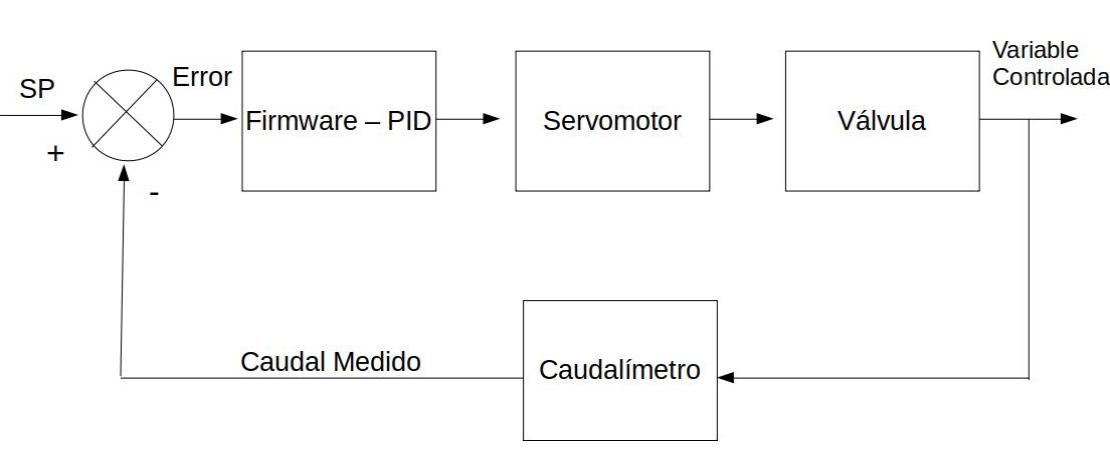
\includegraphics[scale=.45]{./Figures/DiagramaEnBloqueDeControlCeldaPrimaria-V5.png}
\caption{Diagrama en bloque de control - celda primaria.}
\label{fig:CeldaPrimaria}
\end{figure}

\section{Compuertas Miller}
\label{sec:Compuertas miller}
Las compuertas Miller es el mecanismo más utilizado en los canales de agua de riego para controlar la entrada de agua de los canales ramales y tomas directas a las parcelas. Están construidas de fierro fundido (vaciado o colado) por su resistencia a la oxidación. Sin embargo, son frágiles y poco maleables. La toma Miller, en esencia, es una compuerta circular que obtura la entrada a la tubería de salida, la que es izada por un mecanismo elevador compuesto de un vástago cilíndrico con cuerda tipo tornillo (roscas), generalmente de 2” de diámetro y longitud variable, en función de la altura a colocar la toma y un volante. Las tomas-granja Miller se clasifican por el diámetro de la tubería a obturar, y son de 18” y 24” las más comunes para tomas-granjas, mientras que las de 30” y 36” son usadas para abastecer ramales y subramales.
Las ventajas de este tipo de tomas es que son relativamente baratas, la mayoría de las fundidoras las pueden construir y son de fácil colocación. Como desventajas, destacan que pueden tener filtraciones de consideración al ser difícil un cierre hermético debido al metal de la tubería y de la compuerta (comal), especialmente si, durante su fundición, no hay cuidado de tener acabados completamente a nivel. La calibración de esta estructura es difícil, ya que al abrirse parcialmente la compuerta sobre la tubería ambas de figura circular, se forman secciones tipo “media luna” con área hidráulica variable, sin seguir un patrón de fácil cálculo. 
En las figuras \ref{fig:Compuerta tipo miller para toma-granja}, \ref{fig:Conducto preparado para colocar compuerta tipo miller.} y \ref{fig:Toma granja tipo miller de compuerta circular.} se puede apreciar como es la estructura de la compuerta, el conducto para la toma y su colocación.

\begin{figure}[h]
\centering
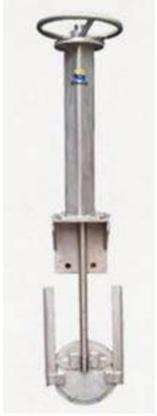
\includegraphics[scale=.65]{./Figures/CompuertaMiller.jpeg}
\caption{Compuerta tipo Miller para toma-granja.}
\label{fig:Compuerta tipo miller para toma-granja}
\end{figure}

\begin{figure}[h]
\centering
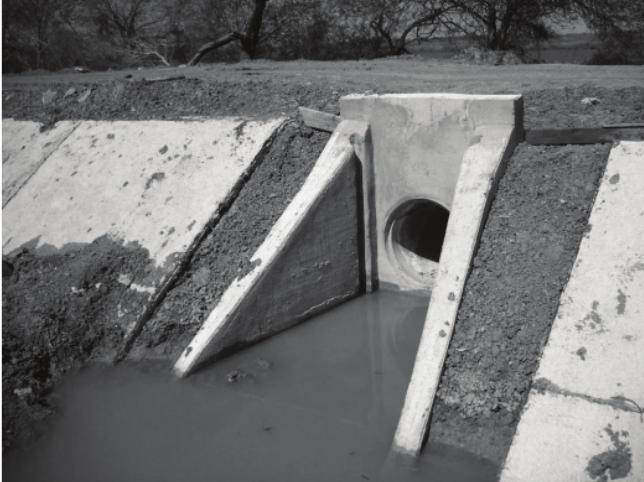
\includegraphics[scale=.58]{./Figures/ConductoPreparadoParaCompuertaMiller.jpeg}
\caption{Conducto preparado para colocar compuerta tipo Miller.}
\label{fig:Conducto preparado para colocar compuerta tipo miller.}
\end{figure}


\begin{figure}[htpb]
\centering
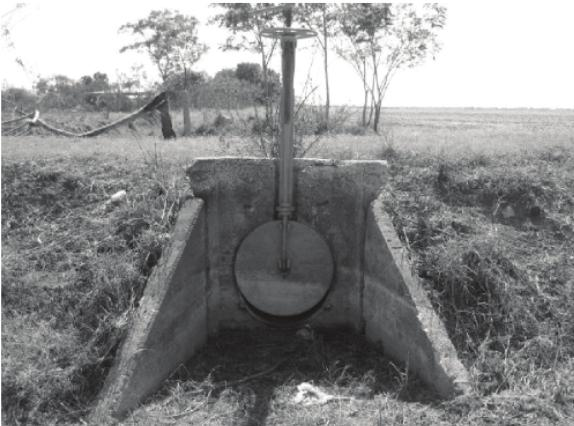
\includegraphics[scale=.65]{./Figures/compuertamillercircular.jpeg}
\caption{Toma-granja tipo Miller de compuerta circular de 18” de diámetro.}
\label{fig:Toma granja tipo miller de compuerta circular.}
\end{figure}

Este mecanismo que se mostró y que se emplea en muchos países para el control de entrada de agua a los canales principales o bien a las parcelas, impulsó a utilizar, en el prototipo a escala, una válvula esférica simulando ser una compuerta Miller.   

\section{Requerimiento a nivel de software y hardware}
\label{sec:ejemplo}
En esta sección se presentan los requerimientos específicos de software y hardware del sistema. Estos se tuvieron en cuenta al momento de inicio del desarrollo de este proyecto, cuyo fin es, mediante el control de movimiento de una válvula regular el caudal de agua según las necesidades del usuario. 
\subsection{Requisitos específicos del software}
\label{subsec:ejemplo}


 Los requisitos específicos de software fueron:

\begin{enumerate}
	\item El firmware deberá generar como señal, trenes de pulsos para controlar el movimiento del eje perteneciente al servomotor.
	\item El firmware deberá determinar, mediante el sensor de presión en conjunto con la placa de aforo triangular, el caudal de agua que fluye a través de este instrumento de medición.
	\item  El firmware deberá incluir un algoritmo de control PID, que por medio de un lazo de retroalimentación permitiese regular la variable a controlar.
	\item El firmware deberá ser capaz, a través de un pin configurado como salida, establecer el sentido de giro del eje del servomotor, horario - antihorario.
	\item El firmware deberá ser capaz, a través de un pin configurado como salida, habilitar - deshabilitar el servomotor.
	\item El firmware deberá interactuar, mediante el empleo del puerto serial, con otra aplicación. 	  
	\item Con un protocolo de comunicación definido entre la aplicación externa y el firmware, este último deberá ser capaz de recibir y enviar datos.
	\item El firmware deberá enviar una notificación de correcta recepción de cualquier comando mediante el envío de un comando específico hacía la aplicación externa.  
	\item El firmware deberá reportar o notificar a la aplicación externa la recepción de un comando inválido mediante un comando específico.
	\item En caso de recepción de comandos válidos, el firmware deberá informar internamente que hay datos a procesar. 
\end{enumerate}

\subsection{Requisitos específicos del hardware}
\label{subsec:requisitoshw}
 Los requisitos específicos principales de hardware fueron:
\begin{enumerate}
	\item Se hará uso de la placa EDU-CIAA-NXP como computadora principal para el prototipo a escala.
	\item Se construirá un mecanizado de  válvula de control estándar mediante un servomotor energizado paso a paso y un elemento medidor de ángulo tipo potenciométrico resistivo.
	\item Se construirá un medidor de caudal por canal de aforo utilizando para la medición de la altura de nivel de agua un sensor MPX5010DP.
	\item Se diseñará y fabricará un circuito como interfaz que controlará las señales enviadas desde la placa EDU-CIAA-NXP al controlador del servomotor paso a paso. 
\end{enumerate}

\section{Características de hardware propias del equipo}
\label{sec:Características propias del equipo}
\subsection{Motor paso a paso y controlador}
Para la construcción de la válvula de control fue preciso emplear un motor  que tenga la capacidad de mover una llave esférica. Para este proyecto, por cuestión de disponibilidad, se utilizó un motor paso a paso y un controlador cuyo modelos son 86HS85 y MA860H respectivamente.
El motor paso a paso de 8 hilos posee un torque nominal de 8,5 Nm, suficiente como para realizar movimientos de apertura parcial o total y cierre total de la carrera de una válvula, según las necesidades requeridas de caudal. 
El driver MA860H es un controlador para motores paso a paso compatibles con motores 86HS85 con las siguientes características principales:

\begin{enumerate}
	\item Permite ajustar la corriente que se dirige hacia el motor.
	\item Posibilita controlar al motor hasta en 200 micropasos.
	\item Frecuencia de entrada de tren de pulso hasta 300 khz. 
	\item Corriente de salida hasta 7.2A.
	\item Entrada TTL compatible y ópticamente aislada.
	\item Soporta modos PUL / DIR y CW / CCW.
\end{enumerate}

El MA860H tiene dos conectores, el conector P1 para conexiones de señales de control y el conector P2 para conexiones de potencia y motor.     
Para el control de la válvula fue necesario un motor que pueda producir un momento de 1 Nm o más. 

\subsubsection{Configuraciones del conector P1}
\begin{itemize}

\item Señal de pulso: esta entrada representa la señal de pulso, activa en cada flanco ascendente o descendente (para este trabajo se encuentra configurado en flanco ascendente). Entre 4V y 5V equivale a un pulso alto, entre 0V y 5V a un pulso bajo. Para una respuesta confiable, el ancho de pulso debe ser superior a 1,5 uS. 

\item Señal de dirección: esta señal tiene niveles de voltaje bajo y alto, que representan dos direcciones de rotación del motor. Para una respuesta de movimiento confiable, la señal de dirección debe estar por delante de la señal de pulso por lo menos 5 uS. Entre 4V y 5V equivale a un pulso alto, entre 0V y 5V a un pulso bajo.

\item Señal de habilitación: esta señal se utiliza para habilitar/deshabilitar el controlador. Nivel alto para habilitar y nivel bajo para inhabilitar al controlador.

\end{itemize}
\subsection{Sensor de presión}
Para monitorizar el nivel de la columna de agua, necesario para determinar el caudal en un determinado instante, se optó por su alta precisión un sensor de presión cuyo modelo es MPX5010DP. Este transductor piezo-resistivo, es un sensor de presión de silicio monolítico que puede ser utilizado en aplicaciones que disponen de un microcontrolador o microprocesador con entradas ADC.
El MPX5010DP entrega a su salida un rango de voltaje entre 0V y 5V, mediante esta información y una fórmula que se expone en el siguiente párrafo se puede estimar la presión hasta un valor de 10 KPa, esto es, una columna de agua de hasta 100 cm de altura.
El dispositivo proporciona una salida lineal como puede se observar en la figura \ref{fig:función de salida del sensor}, extraída de su hoja de datos.

\begin{figure}[h]
\centering
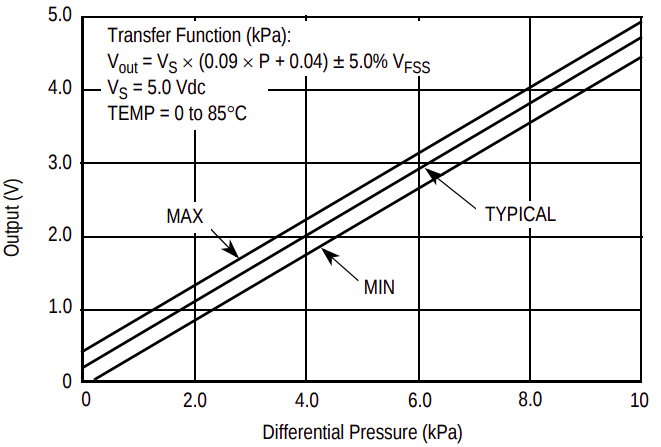
\includegraphics[scale=.55]{./Figures/SalidaMPX5010DP.png}
\caption{Función de salida del sensor de presión MPX5010DP.}
\label{fig:función de salida del sensor}
\end{figure}
Como se pudo observar la función de la figura \ref{fig:función de salida del sensor}, la ecuación para obtener la presión del sensor viene dada por la ecuación \ref{eq:presion}:

\begin{equation}
 \label{eq:presion}
 P = \frac{Vout- 0.04*Vs \pm Tol}{0.09*Vs}
\end{equation}

\vspace{3cm}
Donde:\\
\begin{itemize}
\item Vs: es el valor de voltaje de alimentación, Vs = 5V.\\
\item Vout: es el valor de voltaje que entrega el sensor  a su salida.\\
\item Tol: es la tolerancia, un ajuste que se debe aplicar al sensor para  calibrar a medida.
\end{itemize}

Tomando como base la ecuación de presión diferencial que relaciona la altura se resuelve que (recordando que a la presión atmosférica normal es cero):  

\begin{equation}
 \label{eq:presiónII}
	 P =PH -PL= P = \rho gh =\frac{Vout- 0.04*Vs \pm Tol}{0.09*Vs}	
\end{equation}
 Donde:
 \begin{itemize}
 \item P: es la presión.
 \item $\rho$: es la densidad del agua.
 \item g: es la gravedad.
 \item h: es el nivel de la columna líquida.
 \end{itemize}
 

%\vspace{1cm}
Siendo: 
\begin{itemize}
\item la densidad de agua $\rho$=1000 kg/m3  
\item la aceleración de la gravedad g=10 ms/2
\end{itemize}
la ecuación resultante para obtener h es: 

\begin{equation}
 \label{eq:presión}
	 h = \frac{P}{g*\rho}	
\end{equation}

\vspace{2cm}
La disposición de los pines del dispositivo lo podemos advertir en la figura \ref{fig:disposición de pines del sensor}:
\begin{figure}[h]
\centering
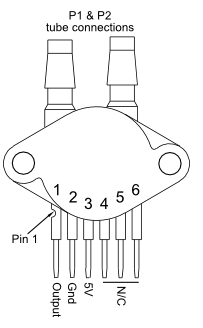
\includegraphics[scale=.65]{./Figures/DisposicionDePinesSensor.png}
\caption{Disposición de pines del sensor de presión MPX5010DP.}
\label{fig:disposición de pines del sensor}
\end{figure}

\section{Planificación}
\label{sec:planificacion}
La planificación original presentada al iniciar el proyecto contemplaba un trabajo de 600 horas. Los atrasos relacionados con la problemática identificada y expuesta en la sección \ref{sec:estructgeneralsistema}, significó repensar un nuevo prototipo con una válvula de control  mecanizada. Esto implicó recurrir a una empresa dedicada a la mecanización de piezas para adaptar el servomotor y una válvula esférica. Como consecuencia de esto, no se pudo contar en tiempo y forma con la pieza total, por lo que se tuvo que modificar la planificación inicial. 
En la tabla \ref{tab:seccplanificacion} se detalla el desglose de tareas pertinente a la planificación original. 
\begin{table}[h]
	\centering
	\caption[Desglose de tareas]{Desglose de tareas}
	\begin{tabular}{l c c}    
		\toprule
		\textbf{WBS}  & \textbf{Tareas} 	 & \textbf{Tiempo[hs]}\\
		\midrule
		1.   & Documentación y Análisis Preliminar	&  19 \\		
		1.1  & Planificación del proyecto			&  24 \\
		1.2  & Análisis de bibliografía especifica &  20 \\
		1.3  & Definición de casos de pruebas		&  15 \\
		2.   & Investigación, Diseño e Implementación & 127 \\
		2.1  & Inicialización del entorno de trabajo  & 34\\
		2.2  & Investigación y diseño del circuito controlador del motor & 12\\
		2.3 & Investigación y diseño del circuito para el sensor lineal &31\\
		2.4 & Definición de la arquitectura del firmware & 54\\
		2.5 & Definición de las interfaces y API’s  &32\\
		2.6 & Implementación de módulo controlador de motor &15\\
		2.7 & Implementación de módulos de adquisición de datos &12\\
		2.8 & Implementación de módulo de comunicación & 16\\
		2.9 & Implementación de herramientas de testing & 18\\
		2.10 & Integración de módulos & 21\\
		2.11 & Investigación  del sensor de presión diferencial & 15\\
		2.12 & Calibración del sensor de presión diferencial y diseño del circuito &13\\
		3. & Verificación y Validación & 48\\
		3.1 & Pruebas unitarias en submódulos &24\\
		3.2 & Pruebas de integración &19\\
		3.3 & Pruebas de Sistema &23\\
		4. & Cierre & 36\\
		4.1 & Elaboración del Informe del proyecto & 24\\
		4.2 & Elaboración de presentación final del proyecto &12\\
		\bottomrule
		\hline
	\end{tabular}
	\label{tab:seccplanificacion}
\end{table}

%Cuando se quiere poner una lista tabulada, se hace así:
%
%\begin{itemize}
%	\item Este es el primer elemento de la lista.
%	\item Este es el segundo elemento de la lista.
%\end{itemize}
%
%Notar el uso de las mayúsculas y el punto al final de cada elemento.
%
%Si se desea poner una lista numerada el formato es este:
%
%\begin{enumerate}
%	\item Este es el primer elemento de la lista.
%	\item Este es el segundo elemento de la lista.
%\end{enumerate}
%
%Notar el uso de las mayúsculas y el punto al final de cada elemento.
%
%\subsection{Este es el título de una subsección}
%\label{subsec:ejemplo}
%
%Se recomienda no utilizar \textbf{texto en negritas} en ningún párrafo, ni tampoco texto \underline{subrayado}. En cambio sí se debe utilizar \textit{texto en itálicas} para palabras en un idioma extranjero, al menos la primera vez que aparecen en el texto. En el caso de palabras que estamos inventando se deben utilizar ``comillas'', así como también para citas textuales. Por ejemplo, un \textit{digital filter} es una especie de ``selector'' que permite separar ciertos componentes armónicos en particular.
%
%La escritura debe ser impersonal. Por ejemplo, no utilizar ``el diseño del firmware lo hice de acuerdo con tal principio'', sino ``el firmware fue diseñado utilizando tal principio''. 
%
%El trabajo es algo que al momento de escribir la memoria se supone que ya está concluido, entonces todo lo que se refiera a hacer el trabajo se narra en tiempo pasado, porque es algo que ya ocurrió. Por ejemplo, "se diseñó el firmware empleando la técnica de test driven development".
%
%En cambio, la memoria es algo que está vivo cada vez que el lector la lee. Por eso transcurre siempre en tiempo presente, como por ejemplo:
%
%``En el presente capítulo se da una visión global sobre las distintas pruebas realizadas y los resultados obtenidos. Se explica el modo en que fueron llevados a cabo los test unitarios y las pruebas del sistema''.
%
%Se recomienda no utilizar una sección de glosario sino colocar la descripción de las abreviaturas como parte del mismo cuerpo del texto. Por ejemplo, RTOS (\textit{Real Time Operating System}, Sistema Operativo de Tiempo Real) o en caso de considerarlo apropiado mediante notas a pie de página.
%
%Si se desea indicar alguna página web utilizar el siguiente formato de referencias bibliográficas, dónde las referencias se detallan en la sección de bibliografía de la memoria, utilizado el formato establecido por IEEE en \citep{IEEE:citation}. Por ejemplo, ``el presente trabajo se basa en la plataforma EDU-CIAA-NXP \citep{CIAA}, la cual...''.
%
%\subsection{Figuras} 
%
%Al insertar figuras en la memoria se deben considerar determinadas pautas. Para empezar, usar siempre tipografía claramente legible. Luego, tener claro que \textbf{es incorrecto} escribir por ejemplo esto: ``El diseño elegido es un cuadrado, como se ve en la siguiente figura:''
%
%\begin{figure}[h]
%\centering
%
\includegraphics[scale=.50]{./Figures/cuadradoAzul.png}
%\end{figure}
%
%La forma correcta de utilizar una figura es con referencias cruzadas, por ejemplo: ``Se eligió utilizar un cuadrado azul para el logo, como puede observarse en la figura \ref{fig:cuadradoAzul}''.
%
%\begin{figure}[ht]
%	\centering
%	
\includegraphics[scale=.45]{./Figures/cuadradoAzul.png}
%	\caption{Ilustración del cuadrado azul que se eligió para el diseño del logo.}
%	\label{fig:cuadradoAzul}
%\end{figure}
%
%El texto de las figuras debe estar siempre en español, excepto que se decida reproducir una figura original tomada de alguna referencia. En ese caso la referencia de la cual se tomó la figura debe ser indicada en el epígrafe de la figura e incluida como una nota al pie, como se ilustra en la figura \ref{fig:palabraIngles}.
%
%\begin{figure}[htpb]
%	\centering
%	
\includegraphics[scale=.3]{./Figures/word.jpeg}
%	\caption{Imagen tomada de la página oficial del procesador\protect\footnotemark.}
%	\label{fig:palabraIngles}
%\end{figure}
%
%\footnotetext{Imagen tomada de \url{https://goo.gl/images/i7C70w}}
%
%La figura y el epígrafe deben conformar una unidad cuyo significado principal pueda ser comprendido por el lector sin necesidad de leer el cuerpo central de la memoria. Para eso es necesario que el epígrafe sea todo lo detallado que corresponda y si en la figura se utilizan abreviaturas entonces aclarar su significado en el epígrafe o en la misma figura.
%
%
%
%\begin{figure}[ht]
%	\centering
%	\includegraphics[scale=.37]{./Figures/questionMark.png}
%	\caption{¿Por qué de pronto aparece esta figura?}
%	\label{fig:questionMark}
%\end{figure}
%
%Nunca colocar una figura en el documento antes de hacer la primera referencia a ella, como se ilustra con la figura \ref{fig:questionMark}, porque sino el lector no comprenderá por qué de pronto aparece la figura en el documento, lo que distraerá su atención.
%
%Otra posibilidad es utilizar el entorno \textit{subfigure} para incluir más de una figura, como se puede ver en la figura \ref{fig:three graphs}. Notar que se pueden referenciar también las figuras internas individualmente de esta manera: \ref{fig:1de3}, \ref{fig:2de3} y \ref{fig:3de3}.
% 
%\begin{figure}[!htpb]
%     \centering
%     \begin{subfigure}[b]{0.3\textwidth}
%         \centering
%         \includegraphics[width=.65\textwidth]{./Figures/questionMark}
%         \caption{Un caption.}
%         \label{fig:1de3}
%     \end{subfigure}
%     \hfill
%     \begin{subfigure}[b]{0.3\textwidth}
%         \centering
%         \includegraphics[width=.65\textwidth]{./Figures/questionMark}
%         \caption{Otro.}
%         \label{fig:2de3}
%     \end{subfigure}
%     \hfill
%     \begin{subfigure}[b]{0.3\textwidth}
%         \centering
%         \includegraphics[width=.65\textwidth]{./Figures/questionMark}
%         \caption{Y otro más.}
%         \label{fig:3de3}
%     \end{subfigure}
%        \caption{Tres gráficos simples}
%        \label{fig:three graphs}
%\end{figure}
%
%El código para generar las imágenes se encuentra disponible para su reutilización en el archivo \file{Chapter2.tex}.
%
%\subsection{Tablas}
%
%Para las tablas utilizar el mismo formato que para las figuras, sólo que el epígrafe se debe colocar arriba de la tabla, como se ilustra en la tabla \ref{tab:peces}. Observar que sólo algunas filas van con líneas visibles y notar el uso de las negritas para los encabezados.  La referencia se logra utilizando el comando \verb|\ref{<label>}| donde label debe estar definida dentro del entorno de la tabla.
%
%\begin{verbatim}
%\begin{table}[h]
%	\centering
%	\caption[caption corto]{caption largo más descriptivo}
%	\begin{tabular}{l c c}    
%		\toprule
%		\textbf{Especie}     & \textbf{Tamaño} & \textbf{Valor}\\
%		\midrule
%		Amphiprion Ocellaris & 10 cm           & \$ 6.000 \\		
%		Hepatus Blue Tang    & 15 cm           & \$ 7.000 \\
%		Zebrasoma Xanthurus  & 12 cm           & \$ 6.800 \\
%		\bottomrule
%		\hline
%	\end{tabular}
%	\label{tab:peces}
%\end{table}
%\end{verbatim}
%
%
%\begin{table}[h]
%	\centering
%	\caption[caption corto]{caption largo más descriptivo}
%	\begin{tabular}{l c c}    
%		\toprule
%		\textbf{Especie} 	 & \textbf{Tamaño} 		& \textbf{Valor}  \\
%		\midrule
%		Amphiprion Ocellaris & 10 cm 				& \$ 6.000 \\		
%		Hepatus Blue Tang	 & 15 cm				& \$ 7.000 \\
%		Zebrasoma Xanthurus	 & 12 cm				& \$ 6.800 \\
%		\bottomrule
%		\hline
%	\end{tabular}
%	\label{tab:peces}
%\end{table}
%
%En cada capítulo se debe reiniciar el número de conteo de las figuras y las tablas, por ejemplo, figura 2.1 o tabla 2.1, pero no se debe reiniciar el conteo en cada sección. Por suerte la plantilla se encarga de esto por nosotros.
%
%\subsection{Ecuaciones}
%\label{sec:Ecuaciones}
%
%Al insertar ecuaciones en la memoria dentro de un entorno \textit{equation}, éstas se numeran en forma automática  y se pueden referir al igual que como se hace con las figuras y tablas, por ejemplo ver la ecuación \ref{eq:metric}.
%
%\begin{equation}
%	\label{eq:metric}
%	ds^2 = c^2 dt^2 \left( \frac{d\sigma^2}{1-k\sigma^2} + \sigma^2\left[ d\theta^2 + \sin^2\theta d\phi^2 \right] \right)
%\end{equation}
%                                                        
%Es importante tener presente que si bien las ecuaciones pueden ser referidas por su número, también es correcto utilizar los dos puntos, como por ejemplo ``la expresión matemática que describe este comportamiento es la siguiente:''
%
%\begin{equation}
%	\label{eq:schrodinger}
%	\frac{\hbar^2}{2m}\nabla^2\Psi + V(\mathbf{r})\Psi = -i\hbar \frac{\partial\Psi}{\partial t}
%\end{equation}
%
%Para generar la ecuación \ref{eq:metric} se utilizó el siguiente código:
%
%\begin{verbatim}
%\begin{equation}
%	\label{eq:metric}
%	ds^2 = c^2 dt^2 \left( \frac{d\sigma^2}{1-k\sigma^2} + 
%	\sigma^2\left[ d\theta^2 + 
%	\sin^2\theta d\phi^2 \right] \right)
%\end{equation}
%\end{verbatim}
%
%Y para la ecuación \ref{eq:schrodinger}:
%
%\begin{verbatim}
%\begin{equation}
%	\label{eq:schrodinger}
%	\frac{\hbar^2}{2m}\nabla^2\Psi + V(\mathbf{r})\Psi = 
%	-i\hbar \frac{\partial\Psi}{\partial t}
%\end{equation}
%
%\end{verbatim} 
%	\chapter{Diseño e implementación} % Main chapter title
En este capítulo se exponen las tomas decisiones relacionadas al diseño e implementación relacionada al hardware y firmware a lo largo del desarrollo del trabajo. 
\label{Chapter3} % Change X to a consecutive number; for referencing this chapter elsewhere, use \ref{ChapterX}

\definecolor{mygreen}{rgb}{0,0.6,0}
\definecolor{mygray}{rgb}{0.5,0.5,0.5}
\definecolor{mymauve}{rgb}{0.58,0,0.82}

%%%%%%%%%%%%%%%%%%%%%%%%%%%%%%%%%%%%%%%%%%%%%%%%%%%%%%%%%%%%%%%%%%%%%%%%%%%%%
% parámetros para configurar el formato del código en los entornos lstlisting
%%%%%%%%%%%%%%%%%%%%%%%%%%%%%%%%%%%%%%%%%%%%%%%%%%%%%%%%%%%%%%%%%%%%%%%%%%%%%
\lstset{ %
  backgroundcolor=\color{white},   % choose the background color; you must add \usepackage{color} or \usepackage{xcolor}
  basicstyle=\footnotesize,        % the size of the fonts that are used for the code
  breakatwhitespace=false,         % sets if automatic breaks should only happen at whitespace
  breaklines=true,                 % sets automatic line breaking
  captionpos=b,                    % sets the caption-position to bottom
  commentstyle=\color{mygreen},    % comment style
  deletekeywords={...},            % if you want to delete keywords from the given language
  %escapeinside={\%*}{*)},          % if you want to add LaTeX within your code
  %extendedchars=true,              % lets you use non-ASCII characters; for 8-bits encodings only, does not work with UTF-8
  %frame=single,	                % adds a frame around the code
  keepspaces=true,                 % keeps spaces in text, useful for keeping indentation of code (possibly needs columns=flexible)
  keywordstyle=\color{blue},       % keyword style
  language=[ANSI]C,                % the language of the code
  %otherkeywords={*,...},           % if you want to add more keywords to the set
  numbers=left,                    % where to put the line-numbers; possible values are (none, left, right)
  numbersep=5pt,                   % how far the line-numbers are from the code
  numberstyle=\tiny\color{mygray}, % the style that is used for the line-numbers
  rulecolor=\color{black},         % if not set, the frame-color may be changed on line-breaks within not-black text (e.g. comments (green here))
  showspaces=false,                % show spaces everywhere adding particular underscores; it overrides 'showstringspaces'
  showstringspaces=false,          % underline spaces within strings only
  showtabs=false,                  % show tabs within strings adding particular underscores
  stepnumber=1,                    % the step between two line-numbers. If it's 1, each line will be numbered
  stringstyle=\color{mymauve},     % string literal style
  tabsize=2,	                   % sets default tabsize to 2 spaces
  title=\lstname,                  % show the filename of files included with \lstinputlisting; also try caption instead of title
  morecomment=[s]{/*}{*/}
}


%----------------------------------------------------------------------------------------
%	SECTION 1
%----------------------------------------------------------------------------------------
\section{Hardware}
\subsection{Construcción de la válvula de control}
\label{subsec:Construcción de la válvula de control}
Para la fabricación del prototipo fue preciso mecanizar una pieza la cual es una caja desmultiplicadora de fuerza que controla una válvula mediante la energización de un servomotor paso a paso. 
Al emplear una válvula de control fue importante estudiar sus características de funcionamiento. 
La válvula es un mecanismo que permite regular el flujo  o caudal, en este caso de agua, entre dos partes del sistema. 
Básicamente la válvula es un ensamblaje compuesto de un cuerpo con conexión a una tubería y de un obturador operado por accionamiento, donde su función principal es variar el caudal del fluido que circula a través de ella, comportándose como un orificio cuya área está continuamente variando. Las válvulas son uno de los instrumentos de control esenciales en la industria.
Debido a su diseño y materiales, las válvulas pueden abrir y cerrar, conectar y desconectar, regular, modular o aislar un enorme  flujo de líquidos y gases.
El obturador determina la característica de caudal de la válvula; es decir, la relación que existe entre la posición del obturador y el caudal de paso del fluido.
El obturador de una válvula, conforme se va desplazando, produce un área de pasaje que posee una determinada relación característica entre la fracción de carrera de la válvula y el correspondiente caudal que escurre a través de la misma. A esa relación se le da el nombre de característica “inherente” de caudal de válvula.
En este trabajo se utilizó una válvula cuya característica inherente es “Tipo de Apertura Rápida”.
Se trata de una característica que produce una variación grande de caudal a través de la válvula con una carrera pequeña. Este tipo de válvula posibilita el pasaje de casi la totalidad del caudal nominal con apenas una abertura de 25 porciento de la carrera total.
Produce una ganancia muy alta a bajas aperturas de carrera y una ganancia muy baja en aperturas por encima de 60 porciento de carrera total. 
La siguiente figura muestra la curva típica de una válvula de apertura rápida.
\begin{figure}[h]
\centering
\includegraphics[scale=.50]{./Figures/funcion-valvula.jpeg}
\caption{Gráfica del caudal en función de la apertura de la válvula.}
\label{fig:grafica caudal vs. caudal}
\end{figure}

\subsection{Servomotor}
\label{subsec:Servomotor}
Para el control de la válvula fue necesario un motor que pueda producir un momento de 1 Nm o más. Para este proyecto, por cuestión de disponibilidad, se utilizó un motor paso a paso y un controlador cuyo modelos son 86HS85 y MA860H respectivamente.
El motor paso a paso de 8 hilos posee un torque nominal de 8,5 Nm, suficiente como para realizar movimientos de apertura parcial o total y cierre total de la carrera de dicha válvula, según las necesidades requeridas de caudal. 
El driver MA860H es un controlador para motores paso a paso compatibles con motores 86HS85 con las siguientes características principales:

\begin{enumerate}
	\item Permite ajustar la corriente que se dirige hacia el motor.
	\item Posibilita controlar al motor hasta en 200 micropasos.
	\item Frecuencia de entrada de tren de pulso hasta 300khz. 
	\item Corriente de salida hasta 7.2A.
	\item Entrada TTL compatible y ópticamente aislada.
	\item Soporta modos PUL / DIR y CW / CCW.
\end{enumerate}
El MA860H tiene dos conectores, el conector P1 para conexiones de señales de control y el conector P2 para conexiones de potencia y motor. 
\subsubsection{Configuraciones del conector P1}
PUL+,PUL-: Señal de pulso: esta entrada representa la señal de pulso, activa en cada flanco ascendente o descendente (para este trabajo se encuentra activo en flanco ascendente); 4-5V equivale a un pulso alto y 0-0.5V a un pulso bajo. Para una respuesta confiable, el ancho de pulso debe ser superior a 1,5 microssegundos. 
DIR+;DIR- : Señal DIR: esta señal tiene niveles de voltaje bajo / alto, que representan dos direcciones de rotación del motor. Para una respuesta de movimiento confiable, la señal DIR debe estar por delante de la señal PUL por lo menos 5 microsegundos. 4-5V cuando DIR-HIGH, 0-0.5V cuando DIR-LOW. 

ENA+;ENA-: Señal de Habilitación: esta señal se utiliza para habilitar/deshabilitar el controlador. Nivel alto (la señal de control NPN, PNP y las señales de control diferencial son por el contrario, es decir, nivel bajo para habilitar) para habilitar al controlador y nivel bajo para inhabilitar al controlador.
\subsubsection{Circuito interfaz del conector de señal de control (P1)}
El controlador MA860H puede aceptar entradas diferenciales y de un solo extremo (incluida la salida de colector abierto y PNP). El MA860H tiene 3 entradas lógicas aisladas ópticamente que están ubicadas en el conector P1 para aceptar señales de control del microcontrolador. Estas entradas están aisladas para minimizar o eliminar los ruidos eléctricos acoplados a las señales de control del variador. En la siguiente "Figura \ref{fig:circuito interfaz}", se ilustra las conexiones a colector abierto.
\begin{figure}[h]
\centering
\includegraphics[scale=.65]{./Figures/circuitointerfaz-driver.jpeg}
\caption{Circuito Interfaz - conexiones de señales a colector abierto.}
\label{fig:circuito interfaz}
\end{figure}
Siguiendo las recomendaciones del fabricante relacionadas a la construcción del circuito interfaz entre el diver y el microcontrolador se diseñó y fabricó el circuito eléctrico que se muestra en la "Figura \ref{fig:esquemático circuito interfaz}".

\begin{figure}
\centering
\includegraphics[scale=.85]{./Figures/esquematico-circuito-interfaz.png}
\caption{Esquemático de Circuito Interfaz entre el microcontrolador y driver.}
\label{fig:esquemático circuito interfaz}
\end{figure}

En el esquemático se puede observar dos etapas, la primera es un circuito negador y la segunda corresponde al circuito de colector abierto NPN.
Por todo lo descrito se puede decir que la etapa de potencia está formada por el circuito interfaz y el controlador del motor paso a paso. 
Es importante mencionar que además del motor paso a paso, la electroválvula está constituida por un sensor resistivo de ángulo, que se encuentra adosado al eje de la válvula. La señal derivada de dicho sensor también es retroalimentada y ofrece una estimación de la posición del obturador de la misma. El sensor resistivo es un potenciómetro de una vuelta de 50K ohm cuyo modelo es 91A-503, Bourns cermet.
En la "Figura \ref{fig:Diagrama en bloque de la celda primaria}", podemos observar un diagrama en bloque general que indica entre otras partes del trabajo, cómo está constituido el servomotor.  

\begin{figure}
\centering
\includegraphics[scale=.65]{./Figures/Diagrama-en-bloque-general-con-servomotor-V2.jpg}
\caption{Diagrama en bloque de la celda primaria.}
\label{fig:Diagrama en bloque de la celda primaria}
\end{figure}
\subsection{Medidor de caudal}
\label{subsec:Medidor de caudal}
La medición del agua es la cuantificación del caudal de agua que pasa por la sección transversal de un río, canal o tubería. También se le conoce como aforo. 
En la mayoría de los casos, la medición del agua resulta de la necesidad de brindar mayor control sobre su uso y distribución. Dicha medición se realiza a través de medidores de caudal. Estos son dispositivos que utilizan diferentes principios mecánicos o físicos para permitir que un flujo de agua pueda ser cuantificado. 
El medidor, que determina la cantidad de fluido que pasa por unidad de tiempo por una sección dada, utilizado en este trabajo para la verificación de caudal de agua proporcionado y además para generar la señal de realimentación correspondiente, es un “Medidor de caudal de Canal Abierto Tipo Aforo”.
Existen varias formas de aforo en canales abiertos, dentro de las principales se encuentran:
\begin{enumerate}
	\item Método volumétrico.
	\item Vertederos.
	\item Canal Parshall. 
	\item Método hidráulico.
\end{enumerate}
Para efectuar el presente trabajo se utilizó el tipo de aforo con vertedero triangular con escotadura en V.
La medición del caudal de las corrientes naturales nunca puede ser exacta debido a que el canal suele ser irregular y por lo tanto es irregular la relación entre nivel y caudal. Los canales de corrientes naturales están también sometidos a cambios debidos a erosión o depósitos. Se pueden obtener cálculos más confiables cuando el caudal pasa a través de una sección donde esos problemas se han limitado. Los vertederos pueden ser definidos como simples aberturas, sobre las cuales un líquido fluye. El término se aplica también a obstáculos en el paso de la corriente y a las excedencias de los embalses. Los vertederos son orificios sin el borde superior y ofrecen las siguientes ventajas en la medición del agua: 

\begin{itemize}
\item Se logra con ellos precisión en los aforos 	
\item La construcción de la estructura es sencilla
\item No son obstruidos por materiales que flotan en el agua 
\item La duración del dispositivo es relativamente larga
\end{itemize}
Los vertederos son utilizados, intensiva y satisfactoriamente en la medición del caudal de pequeños cursos de agua y conductos libres, así como en el control del flujo en galerías y canales.
Para la construcción del vertedero triangular empleado, se precisó de una chapa de hierro plana de 1 mm de espesor, a la que se le  realizó una hendidura de sección triangular, cuyo  valor de ángulo es de 18 grados.
Esta chapa supera los límites del ancho del canal de forma que, ubicándola  verticalmente y en forma transversal al canal, opera como un embalse que por su hendidura sale un flujo de agua.
De esta forma se puede medir en distintos lugares del recorrido del canal, cuál es el caudal real que está pasando por ese punto en particular.  
La "Figura \ref{fig:Placa de aforo}",  muestra la vista de frente de una estructura de un vertedero con escotadura en V. 	
\begin{figure}
\centering
\includegraphics[scale=.85]{./Figures/PlacaDeAforo.jpeg}
\caption{Placa de aforo: vista de frente.}
\label{fig:Placa de aforo}
\end{figure}
La "Figura \ref{fig:Placa de aforo-VistaLateral}", ilustra la vista lateral del vertedero y cómo fluye el líquido por su abertura.
\begin{figure}
\centering
\includegraphics[scale=.85]{./Figures/PlacaDeAforo-VistaLateral.png}
\caption{Placa de aforo: vista lateral.}
\label{fig:Placa de aforo-VistaLateral}
\end{figure}
Entonces, para el calcular el caudal se debe tener en cuenta la siguiente fórmula:
\begin{equation}
 \label{eq:caudal}
 Q = \frac{8}{15}\sqrt{2g} c \tan\alpha  H^\frac{2}{5} 
\end{equation}
	
\begin{figure}
\centering
\includegraphics[scale=.75]{./Figures/DimensionesPlacaAforo.png}
\caption{Placa de aforo: dimensiones.}
\label{fig:Placa de aforo dimensiones}
\end{figure}	

Teniendo en cuenta la ecuación \ref{eq:caudal}
\begin{itemize}
\item Q: es caudal en m3/seg
\item g: coeficiente de gravedad
\item c: coeficiente de descarga
\item alpha: ángulo del vertedero
\item H: nivel de agua en metros

\end{itemize}

Los medidores de caudal con aforo triangular como el utilizado en el presente trabajo, responden a una ecuación del modelo que se expone arriba y la misma se obtuvo empíricamente. En el caso de este proyecto y por tratarse de un prototipo a escala, es un medidor que se usará por única vez, por lo tanto la tabla de calibración del caudalímetro fue obtenida experimentalmente.  
En la "Figura \ref{fig:alturas vertedero}", se detalla la vista de frente del canal con el vertedero triangular y los diversos niveles de altura que se consideraron al momento de realizar las mediciones pertinentes. 

\begin{figure}
\centering
\includegraphics[scale=.75]{./Figures/AlturaVertedero.png}
\caption{Placa de aforo: dimensiones.}
\label{fig:alturas vertedero}
\end{figure}
A partir de la "Figura \ref{fig:alturas vertedero}", se intenta especificar que existe una manguera, la cual uno de sus extremos se conecta a la base del canal y el otro a una de las dos espigas del sensor. Además, se puede advertir los niveles de altura que se deben tener en cuenta. H total corresponde a la altura entre el nivel de agua en un instante dado y la manguera conectada al sensor, H constante se encuentra asociada al nivel de altura que está comprendido entre dicha manguera y el vértice del triángulo del vertedero, y finalmente H variable es la altura que está contenida entre el nivel de agua y el vértice del triángulo de dicho vertedero.    
Por lo tanto, este caudalímetro de canal abierto por sistema de aforo utiliza como medidor de nivel de columna de agua un sensor de presión cuyo modelo es MPX5010DP. 
Este transductor piezo-resistivo, es un sensor de presión de silicio monolítico que puede ser utilizado en aplicaciones que disponen de un microcontrolador o microprocesador con entradas ADC.
El MPX5010DP entrega a su salida un rango de voltaje entre 0v y 5v, mediante esta información y una fórmula que se expone en el siguiente párrafo se puede estimar la presión hasta un valor de 10 KPa, esto es, una columna de agua de hasta 100 cm de altura.
Esta señal proveniente del sensor en conjunto con un algoritmo de control PID, permite regular el caudal de agua en un determinado valor preestablecido. 
El dispositivo proporciona una salida lineal como puede se observar en la "Figura \ref{fig:función de salida del sensor}", extraída de su hoja de datos.

\begin{figure}
\centering
\includegraphics[scale=.55]{./Figures/SalidaMPX5010DP.png}
\caption{Función de salida del sensor de presión MPX5010DP.}
\label{fig:función de salida del sensor}
\end{figure}
Como se pudo observar el gráfico anterior de la "Figura \ref{fig:función de salida del sensor}", la ecuación para obtener la presión del sensor viene dada por la ecuación \ref{eq:presion}:
\begin{equation}
 \label{eq:presion}
 P = \frac{Vout- 0.04*Vs \pm Tol}{0.09*Vs}
\end{equation}
Vs es el valor de voltaje de alimentación Vs = 5v, Vout es el valor de voltaje que entrega el sensor, Tol es la tolerancia, un ajuste que se debe aplicar al sensor para  calibrar a medida.
Tomando como base la ecuación de presión diferencial que relaciona la altura se resuelve que (recordando que la presión a la atmósfera es cero):  

\begin{equation}
 \label{eq:presión}
	 P =PH -PL= P = gh =\frac{Vout- 0.04*Vs \pm Tol}{0.09*Vs}	
\end{equation}
 Donde P es la presión,  es la densidad del agua, g es la gravedad y h es el nivel de la columna líquida.

La disposición de los pines del dispositivo lo podemos advertir en la "Figura \ref{fig:disposición de pines del sensor}":
\begin{figure}
\centering
\includegraphics[scale=.65]{./Figures/DisposicionDePinesSensor.png}
\caption{Disposición de pines del sensor de presión MPX5010DP.}
\label{fig:disposición de pines del sensor}
\end{figure}

Siendo la densidad del agua =1000 kgm3  y la gravedad g=10ms2
La ecuación resultante para obtener h es: h=Pg. 
Una vez construido el prototipo, se realizó una calibración de caudal obteniéndose una tabla Caudal vs Htotal (altura). Por lo que, en el firmware esta tabla es utilizada para obtener el valor de caudal  en lugar de la fórmula presentada.
\section{Software}
\subsection{Arquitectura de software}
\label{subsec:Arquitectura de software}

Durante la definición de la arquitectura de software se seleccionaron dos arquitecturas de software y se integraron para confeccionar una arquitectura híbrida, de modo tal que se adapte a las necesidades concretas de este proyecto. Por un lado, se seleccionó una arquitectura en capas, la cual está conformada por tres capas claramente definidas.
En la capa HAL se encuentran los drivers encargados de abstraer los detalles de acceso al hardware. De esta forma, facilitará la migración a otro microcontrolador en caso de que en el futuro hiciese falta. Adicionalmente, permite una mayor claridad en la implementación, separando los drivers de la lógica de la aplicación.
Debido a que en producción se utilizará como hardware a la CIAA-NXP y durante el desarrollo la EDU-CIAA-NXP, se empleó el firmware de la CIAA versión 3.0 como capa de abstracción de hardware. 
En la capa de aplicación se encuentran todos los componentes que encapsulan la lógica de aplicación, y finalmente, la tercera corresponde al sistema operativo de tiempo real. En esta capa se empleó el sistema operativo FreeRTOS.
El sistema incluye sensores que proveen información relacionada al ámbito a controlar y un actuador que cambian dicho ámbito. Por lo tanto, en respuesta a las alteraciones identificadas por los sensores, se envían señales de control a los actuadores del sistema. Entonces, al identificar que dicho sistema debe poseer este tipo de comportamiento se definió emplear una arquitectura de tiempo real inherente al “Control Ambiental”, ya que este patrón de arquitectura de software brinda la posibilidad de recopilar datos del entorno por medio de sensores como así también el estado en el que se encuentran los actuadores  conectados al sistema. Con base en datos reunidos de sensores y actuador, se envían señales de control hacia el actuador para producir cambios en dicho entorno controlado. En la "Figura \ref{fig:Arquitectura de software}", se puede ver el diagrama del patrón arquitectónico que es la base del diseño del sistema de control, y además utilizado en la capa aplicación. 

\begin{figure}
\centering
\includegraphics[scale=.65]{./Figures/ArquitecturaSoftware.png}
\caption{Arquitectura de sistema de control de caudal de agua en canal a cielo abierto.}
\label{fig:Arquitectura de software}
\end{figure}

Al aplicar ambos patrones se constituyó un patrón híbrido de dos capas. La capa inferior es la capa de abstracción de hardware. La capa superior, pertenece a la aplicación.

\subsection{Componentes de software}
\label{subsec:Componentes de software}
Cada capa de software es considerada un componente de software. Con lo cual se poseen los siguientes componentes:

\begin{itemize}
\item HAL
\item Sistema Operativo
\item Aplicación
\end{itemize}

A su vez, la capa de aplicación está compuesta por los siguientes componentes de software:

\begin{itemize}
\item Monitor sensor de presión.
\item Control servomotor.
\item Monitor válvula.
\item Control de recepción y envío de datos.
\end{itemize}

En la "Figura \ref{fig:Capas de componentes de software}", se puede apreciar el nivel de jerarquía de cada una de las capas siendo la capa HAL la  más baja: 

\begin{figure}
\centering
\includegraphics[scale=.75]{./Figures/JerarquiaDeCapas-Software.png}
\caption{Jerarquía de componentes de software.}
\label{fig:Capas de componentes de software}
\end{figure}
\subsubsection{Diseño detallado}
A continuación se incluye el diseño detallado de cada uno de los componentes de software presentados en la "Figura \ref{fig:Arquitectura de software}".
	\begin{figure}
	\centering
	\includegraphics[scale=.65]{./Figures/Procesomonitorsensordepresion.png}
	\caption{Proceso monitor del sensor de presión.}
	\label{fig:Control servomotor}
	\end{figure}
	
\begin{figure}
	\centering
	\includegraphics[scale=.55]{./Figures/ProcesoControlServo.png}
	\caption{Proceso de control del servomotor.}
	\label{fig:Control servomotor}
	\end{figure}

 	\begin{figure}
	\centering
	\includegraphics[scale=.65]{./Figures/MonitorValvula.png}
	\caption{Proceso monitor válvula.}
	\label{fig:Proceso monitor valvula}
	\end{figure}

	\begin{figure}
	\centering
	\includegraphics[scale=.65]{./Figures/Porcesorecepcionyenviodedatos.png}
	\caption{Proceso de envió y recepción de datos.}
	\label{fig:Proceso De envió y recepción de datos}
	\end{figure}

	
\begin{figure}
	\centering
	\includegraphics[scale=.65]{./Figures/procesocontrolPID.png}
	\caption{Proceso de Control PID.}
	\label{fig:Proceso de Control PID}
	\end{figure}
\subsection{Casos de uso}
\label{subsec:Casos de uso}
Para la etapa de captura de requerimientos funcionales que el sistema debía satisfacer se emplearon casos de uso correspondientes al Lenguaje Unificado Modelado (UML) ya que es de mucha utilidad y permite especificar, visualizar, construir y documentar los requisitos del sistema especialmente en sistemas con un alto grado de interacción hombre/máquina. A continuación se presentan dos casos de uso considerados como principales.

\subsubsection{Caso de uso: detectar el nivel de agua del canal}
\begin{table}[t]
\begin{center}
\begin{tabular}{ | m{4cm} | m{9.5cm} | }
\hline Nombre & Detectar el nivel de agua del canal \\ \hline
1.1 Breve descripción & 
El firmware debe detectar por medio del sensor de presión el nivel de agua existente en el canal. \\ \hline

 1.2 Actor Principal&La aplicación móvil.\\ \hline


 1.3 Disparadores & La recepción de un comando. \\ \hline

Flujo de Eventos& \\ \hline

 2.1 Flujo básico &
El firmware recibe el paquete desde un smartphone  o desde una aplicación de comunicación serial desde una pc. \\ \hline


 2.1.2 Flujo básico &
El firmware deberá desencapsular el comando recibido y extraer los diferentes campos de información. \\ \hline

 2.1.3 Flujo básico &
El firmware deberá identificar el tipo de operación. \\ \hline


 2.1.4 Flujo básico &
El firmware deberá leer un pin configurado como adc asociado al sensor de presión un valor digital. \\ \hline
 

2.1.5 Flujo básico &
Se repite el paso 2.1.4 hasta 5 veces, de forma que el firmware deberá realizar una acumulación de los valores obtenidos. \\ \hline


2.1.6 Flujo básico &
 El firmware con base al acumulador obtenido en el punto anterior deberá, realizar un filtro de promedio móvil.  \\ \hline
 
2.1.7 Flujo básico &
El firmware deberá convertir el valor digital promediado a tensión. \\ \hline 
2.1.8 Flujo básico &
El firmware deberá obtener el nivel de agua con el dato obtenido en el punto anterior empleando una tabla que se obtendrá experimentalmente. \\ \hline
2.1.9 Flujo básico &
El firmware deberá controlar si el resultado se encuentra dentro de las dimensiones establecidas. \\ \hline
2.1.10 Flujo básico &
El firmware deberá enviar por el puerto serial el valor de nivel de agua en cm. \\ \hline
2.2 Flujo alternativo &  \\ \hline


2.2.1 Flujo alternativo  & 
2.1.9 Si la distancia obtenida se encuentra fuera de rango se enviará por la UART “Distancia Fuera de Rango - Verificar el correcto Funcionamiento del  sensor”. \\ \hline

Requisitos Especiales & \\ \hline


Pre - condiciones & \\ \hline
 
4.1 Pre - condiciones & 
El firmware debe estar en estado de correcto funcionamiento. \\ \hline

4.2 Pre - condiciones &
La comunicación serial se debe encontrar en condiciones óptimas para su funcionamiento correcto. \\ \hline

Post- Condiciones &
El firmware deberá quedar operativo y en correcto 
funcionamiento y en condiciones para la recepción de futuros comandos. \\ \hline

\end{tabular}
\caption{ Caso de uso: detectar el nivel de agua del canal.}
\label{tab:coches}
\end{center}
\end{table}

\subsubsection{Caso de uso:establecer un determinado valor de caudal.}

\begin{table}[t]
\begin{center}
\begin{tabular}{ | m{4cm} | m{9cm} | }
\hline 
Nombre & Establecer un determinado de valor de caudal.\\ \hline
1.1 Breve descripción &
El firmware debe establecer un caudal mediante la manipulación de la posición de la válvula de control.\\ \hline
 1.2 Actor Principal & La aplicación móvil.\\ \hline
 1.3 Disparadores & La recepción de un comando \\ \hline
Flujo de Eventos & \\ \hline


 2.1 Flujo básico &
El firmware recibe el paquete desde un smartphone  o desde una aplicación de comunicación serial desde una pc. \\ \hline
 2.1.2 Flujo básico &
El firmware deberá desencapsular el comando recibido y extraer los diferentes campos de información. \\ \hline
 2.1.3 Flujo básico &
El firmware deberá identificar el tipo de operación. \\ \hline


 2.1.4 Flujo básico &
El firmware deberá leer un pin configurado como adc asociado al sensor de presión un valor digital. \\ \hline


2.1.5 Flujo básico &
Se repite el paso 2.1.4 hasta 5 veces, de forma que el firmware deberá realizar una acumulación de los valores obtenidos.\\ \hline
2.1.6 Flujo básico &
 El firmware con base al acumulador obtenido en el punto anterior deberá, realizar un filtro de promedio móvil.  \\ \hline
2.1.7 Flujo básico & 
El firmware deberá convertir el valor digital promediado a tensión.  \\ \hline
2.1.8 Flujo básico & 
El firmware deberá obtener el caudal con el dato obtenido en el punto anterior empleando una tabla que se obtendrá experimentalmente. \\ \hline
2.1.9 Flujo básico &
El firmware deberá comparar este resultado de caudal obtenido con el set point. \\ \hline
2.1.10 Flujo básico &
En caso de ser valores diferentes, el firmware deberá generar un tren de pulsos hasta posicionar la válvula de control. \\ \hline
2.1.11 Flujo básico &
Se repite desde 2.1.4 hasta que el caudal obtenido a través del sensor y el set point sean iguales. \\ \hline
2.2 Flujo alternativo & \\ \hline


2.2.1 Flujo alternativo & 
2.1.10 Si los valores son iguales el firmware deberá detener la generación del tren de pulsos. \\ \hline
Requisitos Especiales & \\ \hline


Pre - condiciones & \\ \hline
 
4.1 Pre - condiciones &
El firmware debe estar en estado de correcto funcionamiento. \\ \hline
4.2 Pre - condiciones &
La comunicación serial se debe encontrar en condiciones óptimas para su funcionamiento correcto. \\ \hline
Post- Condiciones &
El firmware deberá quedar operativo y en correcto funcionamiento y en condiciones para la recepción de futuros comandos.\\ \hline
\end{tabular}
\caption{ Caso de uso: establecer un determinado valor de caudal.}
\label{tab:establecer un determinado valor de caudal.}
\end{center}
\end{table}

\subsection{Diagrama de clase}
\label{subsec:Diagrama de clase}
Al momento de desarrollar el firmware, de forma previa se realizó un diagrama de clase, que se puede ver en la "Figura \ref{fig:Diagrama de clase.}". 
\begin{figure}
	\centering
	\includegraphics[scale=.75]{./Figures/DiagramaDeClase-DistribucionDeAgua.png}
	\caption{Diagrama de clase.}
	\label{fig:Diagrama de clase.}
	\end{figure}

Uart:  
este módulo recibe y envía los comandos desde y hacia la aplicación de comunicación serial que se ejecuta en la PC.

Command Processing:
acumulará y convertirá de carácter a decimal los comandos recibidos y los devuelve cuando sea solicitado



Stepper Motor:
este módulo posee todas las funciones inherentes al control del motor paso a paso. Interactúa con el módulo Servomotor para integrar las características de un servomotor convencional. 

Servomotor:
el propósito de Servomotor es establecer la posición de la válvula realizando una comparación entre el resultado que se va obteniendo del algoritmo de control PID, output y la posición actual de dicha válvula.

PID:  
este módulo implementa un algoritmo de control PID. El mismo es ejecutado cada un segundo para cuantificar el error o desviación que existe entre el valor de caudal medido a través del sensor de presión y el valor deseado. Este valor es solicitado por el módulo Servomotor.
\subsection{Protocolo de comunicación}
\label{subsec:Protocolo de comunicación}
Se definió un paquete de datos  para que el usuario pueda testear todos los comandos que involucre el servomotor y verificar su correcto funcionamiento. A continuación se detalla lo siguiente:
\begin{enumerate}
\item Habilitar o deshabilitar el motor.
\item Establecer los micro pasos (MicroStep).
\item Establecer el sentido de giro(Horario/Antihorario).
\item Cantidad de pasos a realizar.
\item El ángulo a girar.
\item Cantidad de vueltas a girar.
\end{enumerate}
Un vez validado el funcionamiento del servomotor se procedió de estructurar los comandos validos del sistema.
\begin{itemize}
\item Habilitar el motor: ME \\
		\hspace{1cm} M: Motor	\\
		\hspace{1cm} E: Habilitar 
\item Deshabilitar el motor: MD \\
		M: Motor \\
		D: Deshabilitar
\item Establecer los micropasos: MMSF, MMSH, MMS04, MMS08, MMS16, MMS32 \\
		M: Motor \\
		MS: MicroSteps \\
		F: Full step \\
		H: Half step \\
		04: 1/4 step \\
		08: 1/8 step \\
		16: 1/16 step \\
		32: 1/32 step 
\item Establecer el sentido de giro del eje del motor: MTH, MTA.\\
		M: Motor. \\
		T: Turn (giro) \\
		H: Horario. \\
		A: Antihorario \\
		
		‘0’ lógico antihorario \\
		’1' lógico	 horario 		
\item	Establecer la cantidad de pasos: MS1201. \\
		M: Motor \\
		S: Step \\
		1201: 4 dígitos para el número de pasos 
\item	Establece el ángulo de giro del eje del motor: MA0360. \\
		M: Motor \\
		A: Ángulo \\
		0360: 4 dígitos para especificar el valor del ángulo 
\item  Establece la cantidad de vueltas que deberá girar el eje del motor: MFT003. \\
    M: Motor \\
    FT: Full Turns(vueltas completadas) \\
    003: 3 dígitos para especificar el valor de las vueltas completas 
\item Establecer el Set Point del control PID: SP075. \\
   SP: Set Point \\
   075: Porcentaje correspondiente al máximo del caudal 
\item Detectar el nivel de agua: NA(nivel de agua).

\end{itemize}

Al final de cada una de las tramas, se incorpora el carácter de salto de línea que indica el límite final del comando. Una vez recibido el mismo, este pasa a ser procesado por una función, de forma que si presenta un error, el firmware envía por el mismo medio una cadena “comando invalido”, caso contrario “comando válido”. 
\subsection{Algoritmo PID}
\label{subsec:Algoritmo PID}
Durante el diseño del proyecto se identificó la posibilidad de implementar un control de proceso con realimentación. La tarea particular del sistema de control, es la de determinar y actualizar la posición de la válvula a medida que cambian las condiciones de carga hasta que la variable controlada, caudal, alcance el valor deseado, y permanecer allí indefinidamente aún produciéndose perturbaciones externas. Con base a las necesidades expuestas se definió incorporar al firmware un algoritmo de control PID como una herramienta tecnológica que permite cuantificar el error o desviación que existe entre un valor medido y un valor deseado de caudal. El mismo está basado en el algoritmo publicado por Brett Beauregard y se modificó para satisfacer las necesidades concretas del presente proyecto. Es útil destacar que se seleccionó un modo de control que consiste en una combinación de la acción integral con la acción proporcional eliminando la acción derivativa.   
Cuando el control es una válvula la acción derivativa no se utiliza. Porque la parte derivativa tiene justamente la propiedad de actuar en un porcentaje muy elevado de la salida ante variaciones muy pequeñas del error, es decir la entrada. Es la parte del algoritmo que se añadió al final de todo, para acelerar la acción de control. Por la naturaleza matemática    del algoritmo, la acción de control de la parte derivativa es muy elevada en porcentaje aunque el error sea pequeño, ante cualquier variación se establece un porcentaje de salida muy grande. Esto hace que ante cualquier pequeña variación del error, la válvula reaccione ante la salida fuertemente abriéndose y cerrándose. Estos movimientos repetitivos, lógicamente terminan rompiendo la válvula. Es por esto que la acción derivativa no se utiliza cuando el actuador del sistema de control es una válvula. 

%A modo de ejemplo:
%
%\begin{lstlisting}[label=cod:vControl,caption=Pseudocódigo del lazo principal de control.]  % Start your code-block
%
%#define MAX_SENSOR_NUMBER 3
%#define MAX_ALARM_NUMBER  6
%#define MAX_ACTUATOR_NUMBER 6
%
%uint32_t sensorValue[MAX_SENSOR_NUMBER];		
%FunctionalState alarmControl[MAX_ALARM_NUMBER];	//ENABLE or DISABLE
%state_t alarmState[MAX_ALARM_NUMBER];						//ON or OFF
%state_t actuatorState[MAX_ACTUATOR_NUMBER];			//ON or OFF
%
%void vControl() {
%
%	initGlobalVariables();
%	
%	period = 500 ms;
%		
%	while(1) {
%
%		ticks = xTaskGetTickCount();
%		
%		updateSensors();
%		
%		updateAlarms();
%		
%		controlActuators();
%		
%		vTaskDelayUntil(&ticks, period);
%	}
%}
%\end{lstlisting}
%
%
%

%	% Chapter Template

\chapter{Ensayos y Resultados} % Main chapter title

\label{Chapter4} % Change X to a consecutive number; for referencing this chapter elsewhere, use \ref{ChapterX}

%----------------------------------------------------------------------------------------
%	SECTION 1
%----------------------------------------------------------------------------------------

\section{Pruebas funcionales del hardware}
\label{sec:pruebasHW}

La idea de esta sección es explicar cómo se hicieron los ensayos, qué resultados se obtuvieron y analizarlos.
 
%	% Chapter Template

\chapter{Conclusiones} % Main chapter title

\label{Chapter5} % Change X to a consecutive number; for referencing this chapter elsewhere, use \ref{ChapterX}


%----------------------------------------------------------------------------------------

%----------------------------------------------------------------------------------------
%	SECTION 1
%----------------------------------------------------------------------------------------

\section{Conclusiones generales }

La idea de esta sección es resaltar cuáles son los principales aportes del trabajo realizado y cómo se podría continuar. Debe ser especialmente breve y concisa. Es buena idea usar un listado para enumerar los logros obtenidos.

Algunas preguntas que pueden servir para completar este capítulo:

\begin{itemize}
\item ¿Cuál es el grado de cumplimiento de los requerimientos?
\item ¿Cuán fielmente se puedo seguir la planificación original (cronograma incluido)?
\item ¿Se manifestó algunos de los riesgos identificados en la planificación? ¿Fue efectivo el plan de mitigación? ¿Se debió aplicar alguna otra acción no contemplada previamente?
\item Si se debieron hacer modificaciones a lo planificado ¿Cuáles fueron las causas y los efectos?
\item ¿Qué técnicas resultaron útiles para el desarrollo del proyecto y cuáles no tanto?
\end{itemize}


%----------------------------------------------------------------------------------------
%	SECTION 2
%----------------------------------------------------------------------------------------
\section{Próximos pasos}

Acá se indica cómo se podría continuar el trabajo más adelante.
 
%\end{verbatim}
%
%Los apéndices también deben escribirse en archivos .tex separados, que se deben ubicar dentro de la carpeta \emph{Appendices}. Los apéndices vienen comentados por defecto con el caracter \code{\%} y para incluirlos simplemente se debe eliminar dicho caracter.
%
%Finalmente, se encuentra el código para incluir la bibliografía en el documento final.  Este código tampoco debe modificarse. La metodología para trabajar las referencias bibliográficas se desarrolla en la sección \ref{sec:biblio}.
%%----------------------------------------------------------------------------------------
%
%\section{Bibliografía}
%\label{sec:biblio}
%
%Las opciones de formato de la bibliografía se controlan a través del paquete de latex \option{biblatex} que se incluye en la memoria en el archivo memoria.tex.  Estas opciones determinan cómo se generan las citas bibliográficas en el cuerpo del documento y cómo se genera la bibliografía al final de la memoria.
%
%En el preámbulo se puede encontrar el código que incluye el paquete biblatex, que no requiere ninguna modificación del usuario de la plantilla, y que contiene las siguientes opciones:
%
%\begin{lstlisting}
%\usepackage[backend=bibtex,
%	natbib=true, 
%	style=numeric, 
%	sorting=none]
%{biblatex}
%\end{lstlisting}
%
%En el archivo \file{reference.bib} se encuentran las referencias bibliográficas que se pueden citar en el documento.  Para incorporar una nueva cita al documento lo primero es agregarla en este archivo con todos los campos necesario.  Todas las entradas bibliográficas comienzan con $@$ y una palabra que define el formato de la entrada.  Para cada formato existen campos obligatorios que deben completarse. No importa el orden en que las entradas estén definidas en el archivo .bib.  Tampoco es importante el orden en que estén definidos los campos de una entrada bibliográfica. A continuación se muestran algunos ejemplos:
%
%\begin{lstlisting}
%@ARTICLE{ARTICLE:1,
%    AUTHOR="John Doe",
%    TITLE="Title",
%    JOURNAL="Journal",
%    YEAR="2017",
%}
%\end{lstlisting}
%
%
%\begin{lstlisting}
%@BOOK{BOOK:1,
%    AUTHOR="John Doe",
%    TITLE="The Book without Title",
%    PUBLISHER="Dummy Publisher",
%    YEAR="2100",
%}
%\end{lstlisting}
%
%
%\begin{lstlisting}
%@INBOOK{BOOK:2,
%    AUTHOR="John Doe",
%    TITLE="The Book without Title",
%    PUBLISHER="Dummy Publisher",
%    YEAR="2100",
%    PAGES="100-200",
%}
%\end{lstlisting}
%
%
%\begin{lstlisting}
%@MISC{WEBSITE:1,
%    HOWPUBLISHED = "\url{http://example.com}",
%    AUTHOR = "Intel",
%    TITLE = "Example Website",
%    MONTH = "12",
%    YEAR = "1988",
%    URLDATE = {2012-11-26}
%}
%\end{lstlisting}
%
%Se debe notar que los nombres \emph{ARTICLE:1}, \emph{BOOK:1}, \emph{BOOK:2} y \emph{WEBSITE:1} son nombres de fantasía que le sirve al autor del documento para identificar la entrada. En este sentido, se podrían reemplazar por cualquier otro nombre.  Tampoco es necesario poner : seguido de un número, en los ejemplos sólo se incluye como un posible estilo para identificar las entradas.
%
%La entradas se citan en el documento con el comando: 
%
%\begin{verbatim}
%\citep{nombre_de_la_entrada}
%\end{verbatim}
%
%Y cuando se usan, se muestran así: \citep{ARTICLE:1}, \citep{BOOK:1}, \citep{BOOK:2}, \citep{WEBSITE:1}.  Notar cómo se conforma la sección Bibliografía al final del documento. 

%	\chapter{Introducción específica} % Main chapter title

\label{Chapter2}

%----------------------------------------------------------------------------------------
%	SECTION 1
%----------------------------------------------------------------------------------------
%Todos los capítulos deben comenzar con un breve párrafo introductorio que indique cuál es el contenido que se encontrará al leerlo.  La redacción sobre el contenido de la memoria debe hacerse en presente y todo lo referido al proyecto en pasado, siempre de modo impersonal.
En este capítulo se abordarán temas referentes al análisis de la estructura del sistema que se desarrolló, gestión, planificación del trabajo y técnicas relacionadas al sensor empleado.  	 

\section{Estructura general del sistema}
\label{sec:estructgeneralsistema}

%\subsection{Uso de mayúscula inicial para los título de secciones}

%Si en el texto se hace alusión a diferentes partes del trabajo referirse a ellas como capítulo, sección o subsección según corresponda. Por ejemplo: ``En el capítulo \ref{Chapter1} se explica tal cosa'', o ``En la sección \ref{sec:ejemplo} se presenta lo que sea'', o ``En la subsección \ref{subsec:ejemplo} se discute otra cosa''.
 
En un plano para la construcción del prototipo a escala, se pudo reconocer un inconveniente. Al emplear una compuerta que se desplaza verticalmente y ubicada en forma perpendicular al canal, se generarían filtraciones de agua en sus guías de desplazamiento. Como se trata de una maqueta a escala, estas filtraciones provocarían errores considerables al momento de realizar las mediciones relacionadas con la altura de la superficie de agua, y cálculos pertinentes al aplicar el método de aforo por compuerta para determinar el caudal. Por lo tanto, en el sistema no se obtendrían los resultados esperados. En este contexto, el caudal que circularía por debajo de la compuerta sería menor que el que se registraría en el caudalímetro. De esta forma, se obtendrían dos valores de caudales diferentes debido, entre otros factores, a las filtraciones.     
Esto motivó a reemplazar, en el prototipo, la compuerta por una válvula y así eliminar los errores que introducen dichas filtraciones. 
Para el control de la válvula se elaboró un servomotor con el empleo de un motor paso a paso con su correspondiente controlador.
En la figura \ref{fig:Vertedero triangular}, se puede apreciar un vertedero triangular en un canal abierto y una regla que mide el nivel de la superficie de agua.
\begin{figure}[h]
\centering
\includegraphics[scale=.60]{./Figures/VertederoTriangular.png}
\caption{Ilustración de un vertedero triangular ubicado en determinado punto a medir caudal en el canal.}
\label{fig:Vertedero triangular}
\end{figure}

Para medir el caudal, se fabricó un caudalímetro por placa de aforo triangular. Estos tipos de instrumentos, también denominados vertederos, representan un dique o pared que intercepta en un determinado punto una corriente de líquido, en este caso agua, con superficie libre, como se puede apreciar en la figura 2.1 . En general, se utilizan para mantener un nivel de superficie de aguas arriba que no exceda de un valor límite, o bien para medir el caudal de agua circulante por un canal. Este instrumento resulta un medidor de caudal sencillo pero efectivo en canales abiertos. 

El principio de funcionamiento de la celda primaria consiste en establecer el caudal de agua a un valor establecido por el usuario. Para llevar a cabo esto, fue necesario el desarrollo de un firmware que controla el eje de un servomotor. Este se encuentra adherido a una válvula, lo que permite maniobrar su rango de apertura para regular el flujo del fluido según las necesidades.

El diagrama de control correspondiente es el que se muestra en la figura \ref{fig:CeldaPrimaria} donde se aprecia que la salida del servomotor actúa directamente sobre la válvula. Esta puede ser una llave esférica, como es este el caso, o un sistema de cremallera. Este tipo de sistemas se aplican a compuertas verticales, como las que podemos encontrar frecuentemente en los canales de agua a cielo abierto. La salida de la válvula es el flujo controlado de caudal al canal. En este punto se coloca un medidor de caudal. Luego su resultado se compara con el set point, valor de caudal fijado por el usuario. En el sumador, a partir de la diferencia que existe entre el set point y el valor de caudal medido se obtiene una señal de error, que seguidamente se procesa por un algoritmo de control PID para que sea igual a cero.

\begin{figure}[htpb]
\centering
\includegraphics[scale=.45]{./Figures/DiagramaEnBloqueDeControlCeldaPrimaria-V5.png}
\caption{Diagrama en bloque de control - celda primaria.}
\label{fig:CeldaPrimaria}
\end{figure}

\section{Compuertas Miller}
\label{sec:Compuertas miller}
Las compuertas Miller es el mecanismo más utilizado en los canales de agua de riego para controlar la entrada de agua de los canales ramales y tomas directas a las parcelas. Están construidas de fierro fundido (vaciado o colado) por su resistencia a la oxidación. Sin embargo, son frágiles y poco maleables. La toma Miller, en esencia, es una compuerta circular que obtura la entrada a la tubería de salida, la que es izada por un mecanismo elevador compuesto de un vástago cilíndrico con cuerda tipo tornillo (roscas), generalmente de 2” de diámetro y longitud variable, en función de la altura a colocar la toma y un volante. Las tomas-granja Miller se clasifican por el diámetro de la tubería a obturar, y son de 18” y 24” las más comunes para tomas-granjas, mientras que las de 30” y 36” son usadas para abastecer ramales y subramales.
Las ventajas de este tipo de tomas es que son relativamente baratas, la mayoría de las fundidoras las pueden construir y son de fácil colocación. Como desventajas, destacan que pueden tener filtraciones de consideración al ser difícil un cierre hermético debido al metal de la tubería y de la compuerta (comal), especialmente si, durante su fundición, no hay cuidado de tener acabados completamente a nivel. La calibración de esta estructura es difícil, ya que al abrirse parcialmente la compuerta sobre la tubería ambas de figura circular, se forman secciones tipo “media luna” con área hidráulica variable, sin seguir un patrón de fácil cálculo. 
En las figuras \ref{fig:Compuerta tipo miller para toma-granja}, \ref{fig:Conducto preparado para colocar compuerta tipo miller.} y \ref{fig:Toma granja tipo miller de compuerta circular.} se puede apreciar como es la estructura de la compuerta, el conducto para la toma y su colocación.

\begin{figure}[h]
\centering
\includegraphics[scale=.65]{./Figures/CompuertaMiller.jpeg}
\caption{Compuerta tipo Miller para toma-granja.}
\label{fig:Compuerta tipo miller para toma-granja}
\end{figure}

\begin{figure}[h]
\centering
\includegraphics[scale=.58]{./Figures/ConductoPreparadoParaCompuertaMiller.jpeg}
\caption{Conducto preparado para colocar compuerta tipo Miller.}
\label{fig:Conducto preparado para colocar compuerta tipo miller.}
\end{figure}


\begin{figure}[htpb]
\centering
\includegraphics[scale=.65]{./Figures/compuertamillercircular.jpeg}
\caption{Toma-granja tipo Miller de compuerta circular de 18” de diámetro.}
\label{fig:Toma granja tipo miller de compuerta circular.}
\end{figure}

Este mecanismo que se mostró y que se emplea en muchos países para el control de entrada de agua a los canales principales o bien a las parcelas, impulsó a utilizar, en el prototipo a escala, una válvula esférica simulando ser una compuerta Miller.   

\section{Requerimiento a nivel de software y hardware}
\label{sec:ejemplo}
En esta sección se presentan los requerimientos específicos de software y hardware del sistema. Estos se tuvieron en cuenta al momento de inicio del desarrollo de este proyecto, cuyo fin es, mediante el control de movimiento de una válvula regular el caudal de agua según las necesidades del usuario. 
\subsection{Requisitos específicos del software}
\label{subsec:ejemplo}


 Los requisitos específicos de software fueron:

\begin{enumerate}
	\item El firmware deberá generar como señal, trenes de pulsos para controlar el movimiento del eje perteneciente al servomotor.
	\item El firmware deberá determinar, mediante el sensor de presión en conjunto con la placa de aforo triangular, el caudal de agua que fluye a través de este instrumento de medición.
	\item  El firmware deberá incluir un algoritmo de control PID, que por medio de un lazo de retroalimentación permitiese regular la variable a controlar.
	\item El firmware deberá ser capaz, a través de un pin configurado como salida, establecer el sentido de giro del eje del servomotor, horario - antihorario.
	\item El firmware deberá ser capaz, a través de un pin configurado como salida, habilitar - deshabilitar el servomotor.
	\item El firmware deberá interactuar, mediante el empleo del puerto serial, con otra aplicación. 	  
	\item Con un protocolo de comunicación definido entre la aplicación externa y el firmware, este último deberá ser capaz de recibir y enviar datos.
	\item El firmware deberá enviar una notificación de correcta recepción de cualquier comando mediante el envío de un comando específico hacía la aplicación externa.  
	\item El firmware deberá reportar o notificar a la aplicación externa la recepción de un comando inválido mediante un comando específico.
	\item En caso de recepción de comandos válidos, el firmware deberá informar internamente que hay datos a procesar. 
\end{enumerate}

\subsection{Requisitos específicos del hardware}
\label{subsec:requisitoshw}
 Los requisitos específicos principales de hardware fueron:
\begin{enumerate}
	\item Se hará uso de la placa EDU-CIAA-NXP como computadora principal para el prototipo a escala.
	\item Se construirá un mecanizado de  válvula de control estándar mediante un servomotor energizado paso a paso y un elemento medidor de ángulo tipo potenciométrico resistivo.
	\item Se construirá un medidor de caudal por canal de aforo utilizando para la medición de la altura de nivel de agua un sensor MPX5010DP.
	\item Se diseñará y fabricará un circuito como interfaz que controlará las señales enviadas desde la placa EDU-CIAA-NXP al controlador del servomotor paso a paso. 
\end{enumerate}

\section{Características de hardware propias del equipo}
\label{sec:Características propias del equipo}
\subsection{Motor paso a paso y controlador}
Para la construcción de la válvula de control fue preciso emplear un motor  que tenga la capacidad de mover una llave esférica. Para este proyecto, por cuestión de disponibilidad, se utilizó un motor paso a paso y un controlador cuyo modelos son 86HS85 y MA860H respectivamente.
El motor paso a paso de 8 hilos posee un torque nominal de 8,5 Nm, suficiente como para realizar movimientos de apertura parcial o total y cierre total de la carrera de una válvula, según las necesidades requeridas de caudal. 
El driver MA860H es un controlador para motores paso a paso compatibles con motores 86HS85 con las siguientes características principales:

\begin{enumerate}
	\item Permite ajustar la corriente que se dirige hacia el motor.
	\item Posibilita controlar al motor hasta en 200 micropasos.
	\item Frecuencia de entrada de tren de pulso hasta 300 khz. 
	\item Corriente de salida hasta 7.2A.
	\item Entrada TTL compatible y ópticamente aislada.
	\item Soporta modos PUL / DIR y CW / CCW.
\end{enumerate}

El MA860H tiene dos conectores, el conector P1 para conexiones de señales de control y el conector P2 para conexiones de potencia y motor.     
Para el control de la válvula fue necesario un motor que pueda producir un momento de 1 Nm o más. 

\subsubsection{Configuraciones del conector P1}
\begin{itemize}

\item Señal de pulso: esta entrada representa la señal de pulso, activa en cada flanco ascendente o descendente (para este trabajo se encuentra configurado en flanco ascendente). Entre 4V y 5V equivale a un pulso alto, entre 0V y 5V a un pulso bajo. Para una respuesta confiable, el ancho de pulso debe ser superior a 1,5 uS. 

\item Señal de dirección: esta señal tiene niveles de voltaje bajo y alto, que representan dos direcciones de rotación del motor. Para una respuesta de movimiento confiable, la señal de dirección debe estar por delante de la señal de pulso por lo menos 5 uS. Entre 4V y 5V equivale a un pulso alto, entre 0V y 5V a un pulso bajo.

\item Señal de habilitación: esta señal se utiliza para habilitar/deshabilitar el controlador. Nivel alto para habilitar y nivel bajo para inhabilitar al controlador.

\end{itemize}
\subsection{Sensor de presión}
Para monitorizar el nivel de la columna de agua, necesario para determinar el caudal en un determinado instante, se optó por su alta precisión un sensor de presión cuyo modelo es MPX5010DP. Este transductor piezo-resistivo, es un sensor de presión de silicio monolítico que puede ser utilizado en aplicaciones que disponen de un microcontrolador o microprocesador con entradas ADC.
El MPX5010DP entrega a su salida un rango de voltaje entre 0V y 5V, mediante esta información y una fórmula que se expone en el siguiente párrafo se puede estimar la presión hasta un valor de 10 KPa, esto es, una columna de agua de hasta 100 cm de altura.
El dispositivo proporciona una salida lineal como puede se observar en la figura \ref{fig:función de salida del sensor}, extraída de su hoja de datos.

\begin{figure}[h]
\centering
\includegraphics[scale=.55]{./Figures/SalidaMPX5010DP.png}
\caption{Función de salida del sensor de presión MPX5010DP.}
\label{fig:función de salida del sensor}
\end{figure}
Como se pudo observar la función de la figura \ref{fig:función de salida del sensor}, la ecuación para obtener la presión del sensor viene dada por la ecuación \ref{eq:presion}:

\begin{equation}
 \label{eq:presion}
 P = \frac{Vout- 0.04*Vs \pm Tol}{0.09*Vs}
\end{equation}

\vspace{3cm}
Donde:\\
\begin{itemize}
\item Vs: es el valor de voltaje de alimentación, Vs = 5V.\\
\item Vout: es el valor de voltaje que entrega el sensor  a su salida.\\
\item Tol: es la tolerancia, un ajuste que se debe aplicar al sensor para  calibrar a medida.
\end{itemize}

Tomando como base la ecuación de presión diferencial que relaciona la altura se resuelve que (recordando que a la presión atmosférica normal es cero):  

\begin{equation}
 \label{eq:presiónII}
	 P =PH -PL= P = \rho gh =\frac{Vout- 0.04*Vs \pm Tol}{0.09*Vs}	
\end{equation}
 Donde:
 \begin{itemize}
 \item P: es la presión.
 \item $\rho$: es la densidad del agua.
 \item g: es la gravedad.
 \item h: es el nivel de la columna líquida.
 \end{itemize}
 

%\vspace{1cm}
Siendo: 
\begin{itemize}
\item la densidad de agua $\rho$=1000 kg/m3  
\item la aceleración de la gravedad g=10 ms/2
\end{itemize}
la ecuación resultante para obtener h es: 

\begin{equation}
 \label{eq:presión}
	 h = \frac{P}{g*\rho}	
\end{equation}

\vspace{2cm}
La disposición de los pines del dispositivo lo podemos advertir en la figura \ref{fig:disposición de pines del sensor}:
\begin{figure}[h]
\centering
\includegraphics[scale=.65]{./Figures/DisposicionDePinesSensor.png}
\caption{Disposición de pines del sensor de presión MPX5010DP.}
\label{fig:disposición de pines del sensor}
\end{figure}

\section{Planificación}
\label{sec:planificacion}
La planificación original presentada al iniciar el proyecto contemplaba un trabajo de 600 horas. Los atrasos relacionados con la problemática identificada y expuesta en la sección \ref{sec:estructgeneralsistema}, significó repensar un nuevo prototipo con una válvula de control  mecanizada. Esto implicó recurrir a una empresa dedicada a la mecanización de piezas para adaptar el servomotor y una válvula esférica. Como consecuencia de esto, no se pudo contar en tiempo y forma con la pieza total, por lo que se tuvo que modificar la planificación inicial. 
En la tabla \ref{tab:seccplanificacion} se detalla el desglose de tareas pertinente a la planificación original. 
\begin{table}[h]
	\centering
	\caption[Desglose de tareas]{Desglose de tareas}
	\begin{tabular}{l c c}    
		\toprule
		\textbf{WBS}  & \textbf{Tareas} 	 & \textbf{Tiempo[hs]}\\
		\midrule
		1.   & Documentación y Análisis Preliminar	&  19 \\		
		1.1  & Planificación del proyecto			&  24 \\
		1.2  & Análisis de bibliografía especifica &  20 \\
		1.3  & Definición de casos de pruebas		&  15 \\
		2.   & Investigación, Diseño e Implementación & 127 \\
		2.1  & Inicialización del entorno de trabajo  & 34\\
		2.2  & Investigación y diseño del circuito controlador del motor & 12\\
		2.3 & Investigación y diseño del circuito para el sensor lineal &31\\
		2.4 & Definición de la arquitectura del firmware & 54\\
		2.5 & Definición de las interfaces y API’s  &32\\
		2.6 & Implementación de módulo controlador de motor &15\\
		2.7 & Implementación de módulos de adquisición de datos &12\\
		2.8 & Implementación de módulo de comunicación & 16\\
		2.9 & Implementación de herramientas de testing & 18\\
		2.10 & Integración de módulos & 21\\
		2.11 & Investigación  del sensor de presión diferencial & 15\\
		2.12 & Calibración del sensor de presión diferencial y diseño del circuito &13\\
		3. & Verificación y Validación & 48\\
		3.1 & Pruebas unitarias en submódulos &24\\
		3.2 & Pruebas de integración &19\\
		3.3 & Pruebas de Sistema &23\\
		4. & Cierre & 36\\
		4.1 & Elaboración del Informe del proyecto & 24\\
		4.2 & Elaboración de presentación final del proyecto &12\\
		\bottomrule
		\hline
	\end{tabular}
	\label{tab:seccplanificacion}
\end{table}

%Cuando se quiere poner una lista tabulada, se hace así:
%
%\begin{itemize}
%	\item Este es el primer elemento de la lista.
%	\item Este es el segundo elemento de la lista.
%\end{itemize}
%
%Notar el uso de las mayúsculas y el punto al final de cada elemento.
%
%Si se desea poner una lista numerada el formato es este:
%
%\begin{enumerate}
%	\item Este es el primer elemento de la lista.
%	\item Este es el segundo elemento de la lista.
%\end{enumerate}
%
%Notar el uso de las mayúsculas y el punto al final de cada elemento.
%
%\subsection{Este es el título de una subsección}
%\label{subsec:ejemplo}
%
%Se recomienda no utilizar \textbf{texto en negritas} en ningún párrafo, ni tampoco texto \underline{subrayado}. En cambio sí se debe utilizar \textit{texto en itálicas} para palabras en un idioma extranjero, al menos la primera vez que aparecen en el texto. En el caso de palabras que estamos inventando se deben utilizar ``comillas'', así como también para citas textuales. Por ejemplo, un \textit{digital filter} es una especie de ``selector'' que permite separar ciertos componentes armónicos en particular.
%
%La escritura debe ser impersonal. Por ejemplo, no utilizar ``el diseño del firmware lo hice de acuerdo con tal principio'', sino ``el firmware fue diseñado utilizando tal principio''. 
%
%El trabajo es algo que al momento de escribir la memoria se supone que ya está concluido, entonces todo lo que se refiera a hacer el trabajo se narra en tiempo pasado, porque es algo que ya ocurrió. Por ejemplo, "se diseñó el firmware empleando la técnica de test driven development".
%
%En cambio, la memoria es algo que está vivo cada vez que el lector la lee. Por eso transcurre siempre en tiempo presente, como por ejemplo:
%
%``En el presente capítulo se da una visión global sobre las distintas pruebas realizadas y los resultados obtenidos. Se explica el modo en que fueron llevados a cabo los test unitarios y las pruebas del sistema''.
%
%Se recomienda no utilizar una sección de glosario sino colocar la descripción de las abreviaturas como parte del mismo cuerpo del texto. Por ejemplo, RTOS (\textit{Real Time Operating System}, Sistema Operativo de Tiempo Real) o en caso de considerarlo apropiado mediante notas a pie de página.
%
%Si se desea indicar alguna página web utilizar el siguiente formato de referencias bibliográficas, dónde las referencias se detallan en la sección de bibliografía de la memoria, utilizado el formato establecido por IEEE en \citep{IEEE:citation}. Por ejemplo, ``el presente trabajo se basa en la plataforma EDU-CIAA-NXP \citep{CIAA}, la cual...''.
%
%\subsection{Figuras} 
%
%Al insertar figuras en la memoria se deben considerar determinadas pautas. Para empezar, usar siempre tipografía claramente legible. Luego, tener claro que \textbf{es incorrecto} escribir por ejemplo esto: ``El diseño elegido es un cuadrado, como se ve en la siguiente figura:''
%
%\begin{figure}[h]
%\centering
%\includegraphics[scale=.50]{./Figures/cuadradoAzul.png}
%\end{figure}
%
%La forma correcta de utilizar una figura es con referencias cruzadas, por ejemplo: ``Se eligió utilizar un cuadrado azul para el logo, como puede observarse en la figura \ref{fig:cuadradoAzul}''.
%
%\begin{figure}[ht]
%	\centering
%	\includegraphics[scale=.45]{./Figures/cuadradoAzul.png}
%	\caption{Ilustración del cuadrado azul que se eligió para el diseño del logo.}
%	\label{fig:cuadradoAzul}
%\end{figure}
%
%El texto de las figuras debe estar siempre en español, excepto que se decida reproducir una figura original tomada de alguna referencia. En ese caso la referencia de la cual se tomó la figura debe ser indicada en el epígrafe de la figura e incluida como una nota al pie, como se ilustra en la figura \ref{fig:palabraIngles}.
%
%\begin{figure}[htpb]
%	\centering
%	\includegraphics[scale=.3]{./Figures/word.jpeg}
%	\caption{Imagen tomada de la página oficial del procesador\protect\footnotemark.}
%	\label{fig:palabraIngles}
%\end{figure}
%
%\footnotetext{Imagen tomada de \url{https://goo.gl/images/i7C70w}}
%
%La figura y el epígrafe deben conformar una unidad cuyo significado principal pueda ser comprendido por el lector sin necesidad de leer el cuerpo central de la memoria. Para eso es necesario que el epígrafe sea todo lo detallado que corresponda y si en la figura se utilizan abreviaturas entonces aclarar su significado en el epígrafe o en la misma figura.
%
%
%
%\begin{figure}[ht]
%	\centering
%	\includegraphics[scale=.37]{./Figures/questionMark.png}
%	\caption{¿Por qué de pronto aparece esta figura?}
%	\label{fig:questionMark}
%\end{figure}
%
%Nunca colocar una figura en el documento antes de hacer la primera referencia a ella, como se ilustra con la figura \ref{fig:questionMark}, porque sino el lector no comprenderá por qué de pronto aparece la figura en el documento, lo que distraerá su atención.
%
%Otra posibilidad es utilizar el entorno \textit{subfigure} para incluir más de una figura, como se puede ver en la figura \ref{fig:three graphs}. Notar que se pueden referenciar también las figuras internas individualmente de esta manera: \ref{fig:1de3}, \ref{fig:2de3} y \ref{fig:3de3}.
% 
%\begin{figure}[!htpb]
%     \centering
%     \begin{subfigure}[b]{0.3\textwidth}
%         \centering
%         \includegraphics[width=.65\textwidth]{./Figures/questionMark}
%         \caption{Un caption.}
%         \label{fig:1de3}
%     \end{subfigure}
%     \hfill
%     \begin{subfigure}[b]{0.3\textwidth}
%         \centering
%         \includegraphics[width=.65\textwidth]{./Figures/questionMark}
%         \caption{Otro.}
%         \label{fig:2de3}
%     \end{subfigure}
%     \hfill
%     \begin{subfigure}[b]{0.3\textwidth}
%         \centering
%         \includegraphics[width=.65\textwidth]{./Figures/questionMark}
%         \caption{Y otro más.}
%         \label{fig:3de3}
%     \end{subfigure}
%        \caption{Tres gráficos simples}
%        \label{fig:three graphs}
%\end{figure}
%
%El código para generar las imágenes se encuentra disponible para su reutilización en el archivo \file{Chapter2.tex}.
%
%\subsection{Tablas}
%
%Para las tablas utilizar el mismo formato que para las figuras, sólo que el epígrafe se debe colocar arriba de la tabla, como se ilustra en la tabla \ref{tab:peces}. Observar que sólo algunas filas van con líneas visibles y notar el uso de las negritas para los encabezados.  La referencia se logra utilizando el comando \verb|\ref{<label>}| donde label debe estar definida dentro del entorno de la tabla.
%
%\begin{verbatim}
%\begin{table}[h]
%	\centering
%	\caption[caption corto]{caption largo más descriptivo}
%	\begin{tabular}{l c c}    
%		\toprule
%		\textbf{Especie}     & \textbf{Tamaño} & \textbf{Valor}\\
%		\midrule
%		Amphiprion Ocellaris & 10 cm           & \$ 6.000 \\		
%		Hepatus Blue Tang    & 15 cm           & \$ 7.000 \\
%		Zebrasoma Xanthurus  & 12 cm           & \$ 6.800 \\
%		\bottomrule
%		\hline
%	\end{tabular}
%	\label{tab:peces}
%\end{table}
%\end{verbatim}
%
%
%\begin{table}[h]
%	\centering
%	\caption[caption corto]{caption largo más descriptivo}
%	\begin{tabular}{l c c}    
%		\toprule
%		\textbf{Especie} 	 & \textbf{Tamaño} 		& \textbf{Valor}  \\
%		\midrule
%		Amphiprion Ocellaris & 10 cm 				& \$ 6.000 \\		
%		Hepatus Blue Tang	 & 15 cm				& \$ 7.000 \\
%		Zebrasoma Xanthurus	 & 12 cm				& \$ 6.800 \\
%		\bottomrule
%		\hline
%	\end{tabular}
%	\label{tab:peces}
%\end{table}
%
%En cada capítulo se debe reiniciar el número de conteo de las figuras y las tablas, por ejemplo, figura 2.1 o tabla 2.1, pero no se debe reiniciar el conteo en cada sección. Por suerte la plantilla se encarga de esto por nosotros.
%
%\subsection{Ecuaciones}
%\label{sec:Ecuaciones}
%
%Al insertar ecuaciones en la memoria dentro de un entorno \textit{equation}, éstas se numeran en forma automática  y se pueden referir al igual que como se hace con las figuras y tablas, por ejemplo ver la ecuación \ref{eq:metric}.
%
%\begin{equation}
%	\label{eq:metric}
%	ds^2 = c^2 dt^2 \left( \frac{d\sigma^2}{1-k\sigma^2} + \sigma^2\left[ d\theta^2 + \sin^2\theta d\phi^2 \right] \right)
%\end{equation}
%                                                        
%Es importante tener presente que si bien las ecuaciones pueden ser referidas por su número, también es correcto utilizar los dos puntos, como por ejemplo ``la expresión matemática que describe este comportamiento es la siguiente:''
%
%\begin{equation}
%	\label{eq:schrodinger}
%	\frac{\hbar^2}{2m}\nabla^2\Psi + V(\mathbf{r})\Psi = -i\hbar \frac{\partial\Psi}{\partial t}
%\end{equation}
%
%Para generar la ecuación \ref{eq:metric} se utilizó el siguiente código:
%
%\begin{verbatim}
%\begin{equation}
%	\label{eq:metric}
%	ds^2 = c^2 dt^2 \left( \frac{d\sigma^2}{1-k\sigma^2} + 
%	\sigma^2\left[ d\theta^2 + 
%	\sin^2\theta d\phi^2 \right] \right)
%\end{equation}
%\end{verbatim}
%
%Y para la ecuación \ref{eq:schrodinger}:
%
%\begin{verbatim}
%\begin{equation}
%	\label{eq:schrodinger}
%	\frac{\hbar^2}{2m}\nabla^2\Psi + V(\mathbf{r})\Psi = 
%	-i\hbar \frac{\partial\Psi}{\partial t}
%\end{equation}
%
%\end{verbatim} 
%	\chapter{Diseño e implementación} % Main chapter title
En este capítulo se exponen las tomas decisiones relacionadas al diseño e implementación relacionada al hardware y firmware a lo largo del desarrollo del trabajo. 
\label{Chapter3} % Change X to a consecutive number; for referencing this chapter elsewhere, use \ref{ChapterX}

\definecolor{mygreen}{rgb}{0,0.6,0}
\definecolor{mygray}{rgb}{0.5,0.5,0.5}
\definecolor{mymauve}{rgb}{0.58,0,0.82}

%%%%%%%%%%%%%%%%%%%%%%%%%%%%%%%%%%%%%%%%%%%%%%%%%%%%%%%%%%%%%%%%%%%%%%%%%%%%%
% parámetros para configurar el formato del código en los entornos lstlisting
%%%%%%%%%%%%%%%%%%%%%%%%%%%%%%%%%%%%%%%%%%%%%%%%%%%%%%%%%%%%%%%%%%%%%%%%%%%%%
\lstset{ %
  backgroundcolor=\color{white},   % choose the background color; you must add \usepackage{color} or \usepackage{xcolor}
  basicstyle=\footnotesize,        % the size of the fonts that are used for the code
  breakatwhitespace=false,         % sets if automatic breaks should only happen at whitespace
  breaklines=true,                 % sets automatic line breaking
  captionpos=b,                    % sets the caption-position to bottom
  commentstyle=\color{mygreen},    % comment style
  deletekeywords={...},            % if you want to delete keywords from the given language
  %escapeinside={\%*}{*)},          % if you want to add LaTeX within your code
  %extendedchars=true,              % lets you use non-ASCII characters; for 8-bits encodings only, does not work with UTF-8
  %frame=single,	                % adds a frame around the code
  keepspaces=true,                 % keeps spaces in text, useful for keeping indentation of code (possibly needs columns=flexible)
  keywordstyle=\color{blue},       % keyword style
  language=[ANSI]C,                % the language of the code
  %otherkeywords={*,...},           % if you want to add more keywords to the set
  numbers=left,                    % where to put the line-numbers; possible values are (none, left, right)
  numbersep=5pt,                   % how far the line-numbers are from the code
  numberstyle=\tiny\color{mygray}, % the style that is used for the line-numbers
  rulecolor=\color{black},         % if not set, the frame-color may be changed on line-breaks within not-black text (e.g. comments (green here))
  showspaces=false,                % show spaces everywhere adding particular underscores; it overrides 'showstringspaces'
  showstringspaces=false,          % underline spaces within strings only
  showtabs=false,                  % show tabs within strings adding particular underscores
  stepnumber=1,                    % the step between two line-numbers. If it's 1, each line will be numbered
  stringstyle=\color{mymauve},     % string literal style
  tabsize=2,	                   % sets default tabsize to 2 spaces
  title=\lstname,                  % show the filename of files included with \lstinputlisting; also try caption instead of title
  morecomment=[s]{/*}{*/}
}


%----------------------------------------------------------------------------------------
%	SECTION 1
%----------------------------------------------------------------------------------------
\section{Hardware}
\subsection{Construcción de la válvula de control}
\label{subsec:Construcción de la válvula de control}
Para la fabricación del prototipo fue preciso mecanizar una pieza la cual es una caja desmultiplicadora de fuerza que controla una válvula mediante la energización de un servomotor paso a paso. 
Al emplear una válvula de control fue importante estudiar sus características de funcionamiento. 
La válvula es un mecanismo que permite regular el flujo  o caudal, en este caso de agua, entre dos partes del sistema. 
Básicamente la válvula es un ensamblaje compuesto de un cuerpo con conexión a una tubería y de un obturador operado por accionamiento, donde su función principal es variar el caudal del fluido que circula a través de ella, comportándose como un orificio cuya área está continuamente variando. Las válvulas son uno de los instrumentos de control esenciales en la industria.
Debido a su diseño y materiales, las válvulas pueden abrir y cerrar, conectar y desconectar, regular, modular o aislar un enorme  flujo de líquidos y gases.
El obturador determina la característica de caudal de la válvula; es decir, la relación que existe entre la posición del obturador y el caudal de paso del fluido.
El obturador de una válvula, conforme se va desplazando, produce un área de pasaje que posee una determinada relación característica entre la fracción de carrera de la válvula y el correspondiente caudal que escurre a través de la misma. A esa relación se le da el nombre de característica “inherente” de caudal de válvula.
En este trabajo se utilizó una válvula cuya característica inherente es “Tipo de Apertura Rápida”.
Se trata de una característica que produce una variación grande de caudal a través de la válvula con una carrera pequeña. Este tipo de válvula posibilita el pasaje de casi la totalidad del caudal nominal con apenas una abertura de 25 porciento de la carrera total.
Produce una ganancia muy alta a bajas aperturas de carrera y una ganancia muy baja en aperturas por encima de 60 porciento de carrera total. 
La siguiente figura muestra la curva típica de una válvula de apertura rápida.
\begin{figure}[h]
\centering
\includegraphics[scale=.50]{./Figures/funcion-valvula.jpeg}
\caption{Gráfica del caudal en función de la apertura de la válvula.}
\label{fig:grafica caudal vs. caudal}
\end{figure}

\subsection{Servomotor}
\label{subsec:Servomotor}
Para el control de la válvula fue necesario un motor que pueda producir un momento de 1 Nm o más. Para este proyecto, por cuestión de disponibilidad, se utilizó un motor paso a paso y un controlador cuyo modelos son 86HS85 y MA860H respectivamente.
El motor paso a paso de 8 hilos posee un torque nominal de 8,5 Nm, suficiente como para realizar movimientos de apertura parcial o total y cierre total de la carrera de dicha válvula, según las necesidades requeridas de caudal. 
El driver MA860H es un controlador para motores paso a paso compatibles con motores 86HS85 con las siguientes características principales:

\begin{enumerate}
	\item Permite ajustar la corriente que se dirige hacia el motor.
	\item Posibilita controlar al motor hasta en 200 micropasos.
	\item Frecuencia de entrada de tren de pulso hasta 300khz. 
	\item Corriente de salida hasta 7.2A.
	\item Entrada TTL compatible y ópticamente aislada.
	\item Soporta modos PUL / DIR y CW / CCW.
\end{enumerate}
El MA860H tiene dos conectores, el conector P1 para conexiones de señales de control y el conector P2 para conexiones de potencia y motor. 
\subsubsection{Configuraciones del conector P1}
PUL+,PUL-: Señal de pulso: esta entrada representa la señal de pulso, activa en cada flanco ascendente o descendente (para este trabajo se encuentra activo en flanco ascendente); 4-5V equivale a un pulso alto y 0-0.5V a un pulso bajo. Para una respuesta confiable, el ancho de pulso debe ser superior a 1,5 microssegundos. 
DIR+;DIR- : Señal DIR: esta señal tiene niveles de voltaje bajo / alto, que representan dos direcciones de rotación del motor. Para una respuesta de movimiento confiable, la señal DIR debe estar por delante de la señal PUL por lo menos 5 microsegundos. 4-5V cuando DIR-HIGH, 0-0.5V cuando DIR-LOW. 

ENA+;ENA-: Señal de Habilitación: esta señal se utiliza para habilitar/deshabilitar el controlador. Nivel alto (la señal de control NPN, PNP y las señales de control diferencial son por el contrario, es decir, nivel bajo para habilitar) para habilitar al controlador y nivel bajo para inhabilitar al controlador.
\subsubsection{Circuito interfaz del conector de señal de control (P1)}
El controlador MA860H puede aceptar entradas diferenciales y de un solo extremo (incluida la salida de colector abierto y PNP). El MA860H tiene 3 entradas lógicas aisladas ópticamente que están ubicadas en el conector P1 para aceptar señales de control del microcontrolador. Estas entradas están aisladas para minimizar o eliminar los ruidos eléctricos acoplados a las señales de control del variador. En la siguiente "Figura \ref{fig:circuito interfaz}", se ilustra las conexiones a colector abierto.
\begin{figure}[h]
\centering
\includegraphics[scale=.65]{./Figures/circuitointerfaz-driver.jpeg}
\caption{Circuito Interfaz - conexiones de señales a colector abierto.}
\label{fig:circuito interfaz}
\end{figure}
Siguiendo las recomendaciones del fabricante relacionadas a la construcción del circuito interfaz entre el diver y el microcontrolador se diseñó y fabricó el circuito eléctrico que se muestra en la "Figura \ref{fig:esquemático circuito interfaz}".

\begin{figure}
\centering
\includegraphics[scale=.85]{./Figures/esquematico-circuito-interfaz.png}
\caption{Esquemático de Circuito Interfaz entre el microcontrolador y driver.}
\label{fig:esquemático circuito interfaz}
\end{figure}

En el esquemático se puede observar dos etapas, la primera es un circuito negador y la segunda corresponde al circuito de colector abierto NPN.
Por todo lo descrito se puede decir que la etapa de potencia está formada por el circuito interfaz y el controlador del motor paso a paso. 
Es importante mencionar que además del motor paso a paso, la electroválvula está constituida por un sensor resistivo de ángulo, que se encuentra adosado al eje de la válvula. La señal derivada de dicho sensor también es retroalimentada y ofrece una estimación de la posición del obturador de la misma. El sensor resistivo es un potenciómetro de una vuelta de 50K ohm cuyo modelo es 91A-503, Bourns cermet.
En la "Figura \ref{fig:Diagrama en bloque de la celda primaria}", podemos observar un diagrama en bloque general que indica entre otras partes del trabajo, cómo está constituido el servomotor.  

\begin{figure}
\centering
\includegraphics[scale=.65]{./Figures/Diagrama-en-bloque-general-con-servomotor-V2.jpg}
\caption{Diagrama en bloque de la celda primaria.}
\label{fig:Diagrama en bloque de la celda primaria}
\end{figure}
\subsection{Medidor de caudal}
\label{subsec:Medidor de caudal}
La medición del agua es la cuantificación del caudal de agua que pasa por la sección transversal de un río, canal o tubería. También se le conoce como aforo. 
En la mayoría de los casos, la medición del agua resulta de la necesidad de brindar mayor control sobre su uso y distribución. Dicha medición se realiza a través de medidores de caudal. Estos son dispositivos que utilizan diferentes principios mecánicos o físicos para permitir que un flujo de agua pueda ser cuantificado. 
El medidor, que determina la cantidad de fluido que pasa por unidad de tiempo por una sección dada, utilizado en este trabajo para la verificación de caudal de agua proporcionado y además para generar la señal de realimentación correspondiente, es un “Medidor de caudal de Canal Abierto Tipo Aforo”.
Existen varias formas de aforo en canales abiertos, dentro de las principales se encuentran:
\begin{enumerate}
	\item Método volumétrico.
	\item Vertederos.
	\item Canal Parshall. 
	\item Método hidráulico.
\end{enumerate}
Para efectuar el presente trabajo se utilizó el tipo de aforo con vertedero triangular con escotadura en V.
La medición del caudal de las corrientes naturales nunca puede ser exacta debido a que el canal suele ser irregular y por lo tanto es irregular la relación entre nivel y caudal. Los canales de corrientes naturales están también sometidos a cambios debidos a erosión o depósitos. Se pueden obtener cálculos más confiables cuando el caudal pasa a través de una sección donde esos problemas se han limitado. Los vertederos pueden ser definidos como simples aberturas, sobre las cuales un líquido fluye. El término se aplica también a obstáculos en el paso de la corriente y a las excedencias de los embalses. Los vertederos son orificios sin el borde superior y ofrecen las siguientes ventajas en la medición del agua: 

\begin{itemize}
\item Se logra con ellos precisión en los aforos 	
\item La construcción de la estructura es sencilla
\item No son obstruidos por materiales que flotan en el agua 
\item La duración del dispositivo es relativamente larga
\end{itemize}
Los vertederos son utilizados, intensiva y satisfactoriamente en la medición del caudal de pequeños cursos de agua y conductos libres, así como en el control del flujo en galerías y canales.
Para la construcción del vertedero triangular empleado, se precisó de una chapa de hierro plana de 1 mm de espesor, a la que se le  realizó una hendidura de sección triangular, cuyo  valor de ángulo es de 18 grados.
Esta chapa supera los límites del ancho del canal de forma que, ubicándola  verticalmente y en forma transversal al canal, opera como un embalse que por su hendidura sale un flujo de agua.
De esta forma se puede medir en distintos lugares del recorrido del canal, cuál es el caudal real que está pasando por ese punto en particular.  
La "Figura \ref{fig:Placa de aforo}",  muestra la vista de frente de una estructura de un vertedero con escotadura en V. 	
\begin{figure}
\centering
\includegraphics[scale=.85]{./Figures/PlacaDeAforo.jpeg}
\caption{Placa de aforo: vista de frente.}
\label{fig:Placa de aforo}
\end{figure}
La "Figura \ref{fig:Placa de aforo-VistaLateral}", ilustra la vista lateral del vertedero y cómo fluye el líquido por su abertura.
\begin{figure}
\centering
\includegraphics[scale=.85]{./Figures/PlacaDeAforo-VistaLateral.png}
\caption{Placa de aforo: vista lateral.}
\label{fig:Placa de aforo-VistaLateral}
\end{figure}
Entonces, para el calcular el caudal se debe tener en cuenta la siguiente fórmula:
\begin{equation}
 \label{eq:caudal}
 Q = \frac{8}{15}\sqrt{2g} c \tan\alpha  H^\frac{2}{5} 
\end{equation}
	
\begin{figure}
\centering
\includegraphics[scale=.75]{./Figures/DimensionesPlacaAforo.png}
\caption{Placa de aforo: dimensiones.}
\label{fig:Placa de aforo dimensiones}
\end{figure}	

Teniendo en cuenta la ecuación \ref{eq:caudal}
\begin{itemize}
\item Q: es caudal en m3/seg
\item g: coeficiente de gravedad
\item c: coeficiente de descarga
\item alpha: ángulo del vertedero
\item H: nivel de agua en metros

\end{itemize}

Los medidores de caudal con aforo triangular como el utilizado en el presente trabajo, responden a una ecuación del modelo que se expone arriba y la misma se obtuvo empíricamente. En el caso de este proyecto y por tratarse de un prototipo a escala, es un medidor que se usará por única vez, por lo tanto la tabla de calibración del caudalímetro fue obtenida experimentalmente.  
En la "Figura \ref{fig:alturas vertedero}", se detalla la vista de frente del canal con el vertedero triangular y los diversos niveles de altura que se consideraron al momento de realizar las mediciones pertinentes. 

\begin{figure}
\centering
\includegraphics[scale=.75]{./Figures/AlturaVertedero.png}
\caption{Placa de aforo: dimensiones.}
\label{fig:alturas vertedero}
\end{figure}
A partir de la "Figura \ref{fig:alturas vertedero}", se intenta especificar que existe una manguera, la cual uno de sus extremos se conecta a la base del canal y el otro a una de las dos espigas del sensor. Además, se puede advertir los niveles de altura que se deben tener en cuenta. H total corresponde a la altura entre el nivel de agua en un instante dado y la manguera conectada al sensor, H constante se encuentra asociada al nivel de altura que está comprendido entre dicha manguera y el vértice del triángulo del vertedero, y finalmente H variable es la altura que está contenida entre el nivel de agua y el vértice del triángulo de dicho vertedero.    
Por lo tanto, este caudalímetro de canal abierto por sistema de aforo utiliza como medidor de nivel de columna de agua un sensor de presión cuyo modelo es MPX5010DP. 
Este transductor piezo-resistivo, es un sensor de presión de silicio monolítico que puede ser utilizado en aplicaciones que disponen de un microcontrolador o microprocesador con entradas ADC.
El MPX5010DP entrega a su salida un rango de voltaje entre 0v y 5v, mediante esta información y una fórmula que se expone en el siguiente párrafo se puede estimar la presión hasta un valor de 10 KPa, esto es, una columna de agua de hasta 100 cm de altura.
Esta señal proveniente del sensor en conjunto con un algoritmo de control PID, permite regular el caudal de agua en un determinado valor preestablecido. 
El dispositivo proporciona una salida lineal como puede se observar en la "Figura \ref{fig:función de salida del sensor}", extraída de su hoja de datos.

\begin{figure}
\centering
\includegraphics[scale=.55]{./Figures/SalidaMPX5010DP.png}
\caption{Función de salida del sensor de presión MPX5010DP.}
\label{fig:función de salida del sensor}
\end{figure}
Como se pudo observar el gráfico anterior de la "Figura \ref{fig:función de salida del sensor}", la ecuación para obtener la presión del sensor viene dada por la ecuación \ref{eq:presion}:
\begin{equation}
 \label{eq:presion}
 P = \frac{Vout- 0.04*Vs \pm Tol}{0.09*Vs}
\end{equation}
Vs es el valor de voltaje de alimentación Vs = 5v, Vout es el valor de voltaje que entrega el sensor, Tol es la tolerancia, un ajuste que se debe aplicar al sensor para  calibrar a medida.
Tomando como base la ecuación de presión diferencial que relaciona la altura se resuelve que (recordando que la presión a la atmósfera es cero):  

\begin{equation}
 \label{eq:presión}
	 P =PH -PL= P = gh =\frac{Vout- 0.04*Vs \pm Tol}{0.09*Vs}	
\end{equation}
 Donde P es la presión,  es la densidad del agua, g es la gravedad y h es el nivel de la columna líquida.

La disposición de los pines del dispositivo lo podemos advertir en la "Figura \ref{fig:disposición de pines del sensor}":
\begin{figure}
\centering
\includegraphics[scale=.65]{./Figures/DisposicionDePinesSensor.png}
\caption{Disposición de pines del sensor de presión MPX5010DP.}
\label{fig:disposición de pines del sensor}
\end{figure}

Siendo la densidad del agua =1000 kgm3  y la gravedad g=10ms2
La ecuación resultante para obtener h es: h=Pg. 
Una vez construido el prototipo, se realizó una calibración de caudal obteniéndose una tabla Caudal vs Htotal (altura). Por lo que, en el firmware esta tabla es utilizada para obtener el valor de caudal  en lugar de la fórmula presentada.
\section{Software}
\subsection{Arquitectura de software}
\label{subsec:Arquitectura de software}

Durante la definición de la arquitectura de software se seleccionaron dos arquitecturas de software y se integraron para confeccionar una arquitectura híbrida, de modo tal que se adapte a las necesidades concretas de este proyecto. Por un lado, se seleccionó una arquitectura en capas, la cual está conformada por tres capas claramente definidas.
En la capa HAL se encuentran los drivers encargados de abstraer los detalles de acceso al hardware. De esta forma, facilitará la migración a otro microcontrolador en caso de que en el futuro hiciese falta. Adicionalmente, permite una mayor claridad en la implementación, separando los drivers de la lógica de la aplicación.
Debido a que en producción se utilizará como hardware a la CIAA-NXP y durante el desarrollo la EDU-CIAA-NXP, se empleó el firmware de la CIAA versión 3.0 como capa de abstracción de hardware. 
En la capa de aplicación se encuentran todos los componentes que encapsulan la lógica de aplicación, y finalmente, la tercera corresponde al sistema operativo de tiempo real. En esta capa se empleó el sistema operativo FreeRTOS.
El sistema incluye sensores que proveen información relacionada al ámbito a controlar y un actuador que cambian dicho ámbito. Por lo tanto, en respuesta a las alteraciones identificadas por los sensores, se envían señales de control a los actuadores del sistema. Entonces, al identificar que dicho sistema debe poseer este tipo de comportamiento se definió emplear una arquitectura de tiempo real inherente al “Control Ambiental”, ya que este patrón de arquitectura de software brinda la posibilidad de recopilar datos del entorno por medio de sensores como así también el estado en el que se encuentran los actuadores  conectados al sistema. Con base en datos reunidos de sensores y actuador, se envían señales de control hacia el actuador para producir cambios en dicho entorno controlado. En la "Figura \ref{fig:Arquitectura de software}", se puede ver el diagrama del patrón arquitectónico que es la base del diseño del sistema de control, y además utilizado en la capa aplicación. 

\begin{figure}
\centering
\includegraphics[scale=.65]{./Figures/ArquitecturaSoftware.png}
\caption{Arquitectura de sistema de control de caudal de agua en canal a cielo abierto.}
\label{fig:Arquitectura de software}
\end{figure}

Al aplicar ambos patrones se constituyó un patrón híbrido de dos capas. La capa inferior es la capa de abstracción de hardware. La capa superior, pertenece a la aplicación.

\subsection{Componentes de software}
\label{subsec:Componentes de software}
Cada capa de software es considerada un componente de software. Con lo cual se poseen los siguientes componentes:

\begin{itemize}
\item HAL
\item Sistema Operativo
\item Aplicación
\end{itemize}

A su vez, la capa de aplicación está compuesta por los siguientes componentes de software:

\begin{itemize}
\item Monitor sensor de presión.
\item Control servomotor.
\item Monitor válvula.
\item Control de recepción y envío de datos.
\end{itemize}

En la "Figura \ref{fig:Capas de componentes de software}", se puede apreciar el nivel de jerarquía de cada una de las capas siendo la capa HAL la  más baja: 

\begin{figure}
\centering
\includegraphics[scale=.75]{./Figures/JerarquiaDeCapas-Software.png}
\caption{Jerarquía de componentes de software.}
\label{fig:Capas de componentes de software}
\end{figure}
\subsubsection{Diseño detallado}
A continuación se incluye el diseño detallado de cada uno de los componentes de software presentados en la "Figura \ref{fig:Arquitectura de software}".
	\begin{figure}
	\centering
	\includegraphics[scale=.65]{./Figures/Procesomonitorsensordepresion.png}
	\caption{Proceso monitor del sensor de presión.}
	\label{fig:Control servomotor}
	\end{figure}
	
\begin{figure}
	\centering
	\includegraphics[scale=.55]{./Figures/ProcesoControlServo.png}
	\caption{Proceso de control del servomotor.}
	\label{fig:Control servomotor}
	\end{figure}

 	\begin{figure}
	\centering
	\includegraphics[scale=.65]{./Figures/MonitorValvula.png}
	\caption{Proceso monitor válvula.}
	\label{fig:Proceso monitor valvula}
	\end{figure}

	\begin{figure}
	\centering
	\includegraphics[scale=.65]{./Figures/Porcesorecepcionyenviodedatos.png}
	\caption{Proceso de envió y recepción de datos.}
	\label{fig:Proceso De envió y recepción de datos}
	\end{figure}

	
\begin{figure}
	\centering
	\includegraphics[scale=.65]{./Figures/procesocontrolPID.png}
	\caption{Proceso de Control PID.}
	\label{fig:Proceso de Control PID}
	\end{figure}
\subsection{Casos de uso}
\label{subsec:Casos de uso}
Para la etapa de captura de requerimientos funcionales que el sistema debía satisfacer se emplearon casos de uso correspondientes al Lenguaje Unificado Modelado (UML) ya que es de mucha utilidad y permite especificar, visualizar, construir y documentar los requisitos del sistema especialmente en sistemas con un alto grado de interacción hombre/máquina. A continuación se presentan dos casos de uso considerados como principales.

\subsubsection{Caso de uso: detectar el nivel de agua del canal}
\begin{table}[t]
\begin{center}
\begin{tabular}{ | m{4cm} | m{9.5cm} | }
\hline Nombre & Detectar el nivel de agua del canal \\ \hline
1.1 Breve descripción & 
El firmware debe detectar por medio del sensor de presión el nivel de agua existente en el canal. \\ \hline

 1.2 Actor Principal&La aplicación móvil.\\ \hline


 1.3 Disparadores & La recepción de un comando. \\ \hline

Flujo de Eventos& \\ \hline

 2.1 Flujo básico &
El firmware recibe el paquete desde un smartphone  o desde una aplicación de comunicación serial desde una pc. \\ \hline


 2.1.2 Flujo básico &
El firmware deberá desencapsular el comando recibido y extraer los diferentes campos de información. \\ \hline

 2.1.3 Flujo básico &
El firmware deberá identificar el tipo de operación. \\ \hline


 2.1.4 Flujo básico &
El firmware deberá leer un pin configurado como adc asociado al sensor de presión un valor digital. \\ \hline
 

2.1.5 Flujo básico &
Se repite el paso 2.1.4 hasta 5 veces, de forma que el firmware deberá realizar una acumulación de los valores obtenidos. \\ \hline


2.1.6 Flujo básico &
 El firmware con base al acumulador obtenido en el punto anterior deberá, realizar un filtro de promedio móvil.  \\ \hline
 
2.1.7 Flujo básico &
El firmware deberá convertir el valor digital promediado a tensión. \\ \hline 
2.1.8 Flujo básico &
El firmware deberá obtener el nivel de agua con el dato obtenido en el punto anterior empleando una tabla que se obtendrá experimentalmente. \\ \hline
2.1.9 Flujo básico &
El firmware deberá controlar si el resultado se encuentra dentro de las dimensiones establecidas. \\ \hline
2.1.10 Flujo básico &
El firmware deberá enviar por el puerto serial el valor de nivel de agua en cm. \\ \hline
2.2 Flujo alternativo &  \\ \hline


2.2.1 Flujo alternativo  & 
2.1.9 Si la distancia obtenida se encuentra fuera de rango se enviará por la UART “Distancia Fuera de Rango - Verificar el correcto Funcionamiento del  sensor”. \\ \hline

Requisitos Especiales & \\ \hline


Pre - condiciones & \\ \hline
 
4.1 Pre - condiciones & 
El firmware debe estar en estado de correcto funcionamiento. \\ \hline

4.2 Pre - condiciones &
La comunicación serial se debe encontrar en condiciones óptimas para su funcionamiento correcto. \\ \hline

Post- Condiciones &
El firmware deberá quedar operativo y en correcto 
funcionamiento y en condiciones para la recepción de futuros comandos. \\ \hline

\end{tabular}
\caption{ Caso de uso: detectar el nivel de agua del canal.}
\label{tab:coches}
\end{center}
\end{table}

\subsubsection{Caso de uso:establecer un determinado valor de caudal.}

\begin{table}[t]
\begin{center}
\begin{tabular}{ | m{4cm} | m{9cm} | }
\hline 
Nombre & Establecer un determinado de valor de caudal.\\ \hline
1.1 Breve descripción &
El firmware debe establecer un caudal mediante la manipulación de la posición de la válvula de control.\\ \hline
 1.2 Actor Principal & La aplicación móvil.\\ \hline
 1.3 Disparadores & La recepción de un comando \\ \hline
Flujo de Eventos & \\ \hline


 2.1 Flujo básico &
El firmware recibe el paquete desde un smartphone  o desde una aplicación de comunicación serial desde una pc. \\ \hline
 2.1.2 Flujo básico &
El firmware deberá desencapsular el comando recibido y extraer los diferentes campos de información. \\ \hline
 2.1.3 Flujo básico &
El firmware deberá identificar el tipo de operación. \\ \hline


 2.1.4 Flujo básico &
El firmware deberá leer un pin configurado como adc asociado al sensor de presión un valor digital. \\ \hline


2.1.5 Flujo básico &
Se repite el paso 2.1.4 hasta 5 veces, de forma que el firmware deberá realizar una acumulación de los valores obtenidos.\\ \hline
2.1.6 Flujo básico &
 El firmware con base al acumulador obtenido en el punto anterior deberá, realizar un filtro de promedio móvil.  \\ \hline
2.1.7 Flujo básico & 
El firmware deberá convertir el valor digital promediado a tensión.  \\ \hline
2.1.8 Flujo básico & 
El firmware deberá obtener el caudal con el dato obtenido en el punto anterior empleando una tabla que se obtendrá experimentalmente. \\ \hline
2.1.9 Flujo básico &
El firmware deberá comparar este resultado de caudal obtenido con el set point. \\ \hline
2.1.10 Flujo básico &
En caso de ser valores diferentes, el firmware deberá generar un tren de pulsos hasta posicionar la válvula de control. \\ \hline
2.1.11 Flujo básico &
Se repite desde 2.1.4 hasta que el caudal obtenido a través del sensor y el set point sean iguales. \\ \hline
2.2 Flujo alternativo & \\ \hline


2.2.1 Flujo alternativo & 
2.1.10 Si los valores son iguales el firmware deberá detener la generación del tren de pulsos. \\ \hline
Requisitos Especiales & \\ \hline


Pre - condiciones & \\ \hline
 
4.1 Pre - condiciones &
El firmware debe estar en estado de correcto funcionamiento. \\ \hline
4.2 Pre - condiciones &
La comunicación serial se debe encontrar en condiciones óptimas para su funcionamiento correcto. \\ \hline
Post- Condiciones &
El firmware deberá quedar operativo y en correcto funcionamiento y en condiciones para la recepción de futuros comandos.\\ \hline
\end{tabular}
\caption{ Caso de uso: establecer un determinado valor de caudal.}
\label{tab:establecer un determinado valor de caudal.}
\end{center}
\end{table}

\subsection{Diagrama de clase}
\label{subsec:Diagrama de clase}
Al momento de desarrollar el firmware, de forma previa se realizó un diagrama de clase, que se puede ver en la "Figura \ref{fig:Diagrama de clase.}". 
\begin{figure}
	\centering
	\includegraphics[scale=.75]{./Figures/DiagramaDeClase-DistribucionDeAgua.png}
	\caption{Diagrama de clase.}
	\label{fig:Diagrama de clase.}
	\end{figure}

Uart:  
este módulo recibe y envía los comandos desde y hacia la aplicación de comunicación serial que se ejecuta en la PC.

Command Processing:
acumulará y convertirá de carácter a decimal los comandos recibidos y los devuelve cuando sea solicitado



Stepper Motor:
este módulo posee todas las funciones inherentes al control del motor paso a paso. Interactúa con el módulo Servomotor para integrar las características de un servomotor convencional. 

Servomotor:
el propósito de Servomotor es establecer la posición de la válvula realizando una comparación entre el resultado que se va obteniendo del algoritmo de control PID, output y la posición actual de dicha válvula.

PID:  
este módulo implementa un algoritmo de control PID. El mismo es ejecutado cada un segundo para cuantificar el error o desviación que existe entre el valor de caudal medido a través del sensor de presión y el valor deseado. Este valor es solicitado por el módulo Servomotor.
\subsection{Protocolo de comunicación}
\label{subsec:Protocolo de comunicación}
Se definió un paquete de datos  para que el usuario pueda testear todos los comandos que involucre el servomotor y verificar su correcto funcionamiento. A continuación se detalla lo siguiente:
\begin{enumerate}
\item Habilitar o deshabilitar el motor.
\item Establecer los micro pasos (MicroStep).
\item Establecer el sentido de giro(Horario/Antihorario).
\item Cantidad de pasos a realizar.
\item El ángulo a girar.
\item Cantidad de vueltas a girar.
\end{enumerate}
Un vez validado el funcionamiento del servomotor se procedió de estructurar los comandos validos del sistema.
\begin{itemize}
\item Habilitar el motor: ME \\
		\hspace{1cm} M: Motor	\\
		\hspace{1cm} E: Habilitar 
\item Deshabilitar el motor: MD \\
		M: Motor \\
		D: Deshabilitar
\item Establecer los micropasos: MMSF, MMSH, MMS04, MMS08, MMS16, MMS32 \\
		M: Motor \\
		MS: MicroSteps \\
		F: Full step \\
		H: Half step \\
		04: 1/4 step \\
		08: 1/8 step \\
		16: 1/16 step \\
		32: 1/32 step 
\item Establecer el sentido de giro del eje del motor: MTH, MTA.\\
		M: Motor. \\
		T: Turn (giro) \\
		H: Horario. \\
		A: Antihorario \\
		
		‘0’ lógico antihorario \\
		’1' lógico	 horario 		
\item	Establecer la cantidad de pasos: MS1201. \\
		M: Motor \\
		S: Step \\
		1201: 4 dígitos para el número de pasos 
\item	Establece el ángulo de giro del eje del motor: MA0360. \\
		M: Motor \\
		A: Ángulo \\
		0360: 4 dígitos para especificar el valor del ángulo 
\item  Establece la cantidad de vueltas que deberá girar el eje del motor: MFT003. \\
    M: Motor \\
    FT: Full Turns(vueltas completadas) \\
    003: 3 dígitos para especificar el valor de las vueltas completas 
\item Establecer el Set Point del control PID: SP075. \\
   SP: Set Point \\
   075: Porcentaje correspondiente al máximo del caudal 
\item Detectar el nivel de agua: NA(nivel de agua).

\end{itemize}

Al final de cada una de las tramas, se incorpora el carácter de salto de línea que indica el límite final del comando. Una vez recibido el mismo, este pasa a ser procesado por una función, de forma que si presenta un error, el firmware envía por el mismo medio una cadena “comando invalido”, caso contrario “comando válido”. 
\subsection{Algoritmo PID}
\label{subsec:Algoritmo PID}
Durante el diseño del proyecto se identificó la posibilidad de implementar un control de proceso con realimentación. La tarea particular del sistema de control, es la de determinar y actualizar la posición de la válvula a medida que cambian las condiciones de carga hasta que la variable controlada, caudal, alcance el valor deseado, y permanecer allí indefinidamente aún produciéndose perturbaciones externas. Con base a las necesidades expuestas se definió incorporar al firmware un algoritmo de control PID como una herramienta tecnológica que permite cuantificar el error o desviación que existe entre un valor medido y un valor deseado de caudal. El mismo está basado en el algoritmo publicado por Brett Beauregard y se modificó para satisfacer las necesidades concretas del presente proyecto. Es útil destacar que se seleccionó un modo de control que consiste en una combinación de la acción integral con la acción proporcional eliminando la acción derivativa.   
Cuando el control es una válvula la acción derivativa no se utiliza. Porque la parte derivativa tiene justamente la propiedad de actuar en un porcentaje muy elevado de la salida ante variaciones muy pequeñas del error, es decir la entrada. Es la parte del algoritmo que se añadió al final de todo, para acelerar la acción de control. Por la naturaleza matemática    del algoritmo, la acción de control de la parte derivativa es muy elevada en porcentaje aunque el error sea pequeño, ante cualquier variación se establece un porcentaje de salida muy grande. Esto hace que ante cualquier pequeña variación del error, la válvula reaccione ante la salida fuertemente abriéndose y cerrándose. Estos movimientos repetitivos, lógicamente terminan rompiendo la válvula. Es por esto que la acción derivativa no se utiliza cuando el actuador del sistema de control es una válvula. 

%A modo de ejemplo:
%
%\begin{lstlisting}[label=cod:vControl,caption=Pseudocódigo del lazo principal de control.]  % Start your code-block
%
%#define MAX_SENSOR_NUMBER 3
%#define MAX_ALARM_NUMBER  6
%#define MAX_ACTUATOR_NUMBER 6
%
%uint32_t sensorValue[MAX_SENSOR_NUMBER];		
%FunctionalState alarmControl[MAX_ALARM_NUMBER];	//ENABLE or DISABLE
%state_t alarmState[MAX_ALARM_NUMBER];						//ON or OFF
%state_t actuatorState[MAX_ACTUATOR_NUMBER];			//ON or OFF
%
%void vControl() {
%
%	initGlobalVariables();
%	
%	period = 500 ms;
%		
%	while(1) {
%
%		ticks = xTaskGetTickCount();
%		
%		updateSensors();
%		
%		updateAlarms();
%		
%		controlActuators();
%		
%		vTaskDelayUntil(&ticks, period);
%	}
%}
%\end{lstlisting}
%
%
%

%	% Chapter Template

\chapter{Ensayos y Resultados} % Main chapter title

\label{Chapter4} % Change X to a consecutive number; for referencing this chapter elsewhere, use \ref{ChapterX}

%----------------------------------------------------------------------------------------
%	SECTION 1
%----------------------------------------------------------------------------------------

\section{Pruebas funcionales del hardware}
\label{sec:pruebasHW}

La idea de esta sección es explicar cómo se hicieron los ensayos, qué resultados se obtuvieron y analizarlos.
 
%	% Chapter Template

\chapter{Conclusiones} % Main chapter title

\label{Chapter5} % Change X to a consecutive number; for referencing this chapter elsewhere, use \ref{ChapterX}


%----------------------------------------------------------------------------------------

%----------------------------------------------------------------------------------------
%	SECTION 1
%----------------------------------------------------------------------------------------

\section{Conclusiones generales }

La idea de esta sección es resaltar cuáles son los principales aportes del trabajo realizado y cómo se podría continuar. Debe ser especialmente breve y concisa. Es buena idea usar un listado para enumerar los logros obtenidos.

Algunas preguntas que pueden servir para completar este capítulo:

\begin{itemize}
\item ¿Cuál es el grado de cumplimiento de los requerimientos?
\item ¿Cuán fielmente se puedo seguir la planificación original (cronograma incluido)?
\item ¿Se manifestó algunos de los riesgos identificados en la planificación? ¿Fue efectivo el plan de mitigación? ¿Se debió aplicar alguna otra acción no contemplada previamente?
\item Si se debieron hacer modificaciones a lo planificado ¿Cuáles fueron las causas y los efectos?
\item ¿Qué técnicas resultaron útiles para el desarrollo del proyecto y cuáles no tanto?
\end{itemize}


%----------------------------------------------------------------------------------------
%	SECTION 2
%----------------------------------------------------------------------------------------
\section{Próximos pasos}

Acá se indica cómo se podría continuar el trabajo más adelante.
 
%\end{verbatim}
%
%Los apéndices también deben escribirse en archivos .tex separados, que se deben ubicar dentro de la carpeta \emph{Appendices}. Los apéndices vienen comentados por defecto con el caracter \code{\%} y para incluirlos simplemente se debe eliminar dicho caracter.
%
%Finalmente, se encuentra el código para incluir la bibliografía en el documento final.  Este código tampoco debe modificarse. La metodología para trabajar las referencias bibliográficas se desarrolla en la sección \ref{sec:biblio}.
%%----------------------------------------------------------------------------------------
%
%\section{Bibliografía}
%\label{sec:biblio}
%
%Las opciones de formato de la bibliografía se controlan a través del paquete de latex \option{biblatex} que se incluye en la memoria en el archivo memoria.tex.  Estas opciones determinan cómo se generan las citas bibliográficas en el cuerpo del documento y cómo se genera la bibliografía al final de la memoria.
%
%En el preámbulo se puede encontrar el código que incluye el paquete biblatex, que no requiere ninguna modificación del usuario de la plantilla, y que contiene las siguientes opciones:
%
%\begin{lstlisting}
%\usepackage[backend=bibtex,
%	natbib=true, 
%	style=numeric, 
%	sorting=none]
%{biblatex}
%\end{lstlisting}
%
%En el archivo \file{reference.bib} se encuentran las referencias bibliográficas que se pueden citar en el documento.  Para incorporar una nueva cita al documento lo primero es agregarla en este archivo con todos los campos necesario.  Todas las entradas bibliográficas comienzan con $@$ y una palabra que define el formato de la entrada.  Para cada formato existen campos obligatorios que deben completarse. No importa el orden en que las entradas estén definidas en el archivo .bib.  Tampoco es importante el orden en que estén definidos los campos de una entrada bibliográfica. A continuación se muestran algunos ejemplos:
%
%\begin{lstlisting}
%@ARTICLE{ARTICLE:1,
%    AUTHOR="John Doe",
%    TITLE="Title",
%    JOURNAL="Journal",
%    YEAR="2017",
%}
%\end{lstlisting}
%
%
%\begin{lstlisting}
%@BOOK{BOOK:1,
%    AUTHOR="John Doe",
%    TITLE="The Book without Title",
%    PUBLISHER="Dummy Publisher",
%    YEAR="2100",
%}
%\end{lstlisting}
%
%
%\begin{lstlisting}
%@INBOOK{BOOK:2,
%    AUTHOR="John Doe",
%    TITLE="The Book without Title",
%    PUBLISHER="Dummy Publisher",
%    YEAR="2100",
%    PAGES="100-200",
%}
%\end{lstlisting}
%
%
%\begin{lstlisting}
%@MISC{WEBSITE:1,
%    HOWPUBLISHED = "\url{http://example.com}",
%    AUTHOR = "Intel",
%    TITLE = "Example Website",
%    MONTH = "12",
%    YEAR = "1988",
%    URLDATE = {2012-11-26}
%}
%\end{lstlisting}
%
%Se debe notar que los nombres \emph{ARTICLE:1}, \emph{BOOK:1}, \emph{BOOK:2} y \emph{WEBSITE:1} son nombres de fantasía que le sirve al autor del documento para identificar la entrada. En este sentido, se podrían reemplazar por cualquier otro nombre.  Tampoco es necesario poner : seguido de un número, en los ejemplos sólo se incluye como un posible estilo para identificar las entradas.
%
%La entradas se citan en el documento con el comando: 
%
%\begin{verbatim}
%\citep{nombre_de_la_entrada}
%\end{verbatim}
%
%Y cuando se usan, se muestran así: \citep{ARTICLE:1}, \citep{BOOK:1}, \citep{BOOK:2}, \citep{WEBSITE:1}.  Notar cómo se conforma la sección Bibliografía al final del documento. 
